\documentclass[12pt,letterpaper,oneside,openright]{book}
\usepackage[T1]{fontenc}
\usepackage[utf8]{inputenc}
\usepackage[square]{natbib}
\usepackage[french]{babel}
\bibliographystyle{authordate2}
%\bibliographystyle{plainnat}
\usepackage{amsmath}
\usepackage{mathtools}
\usepackage{amsfonts}
\usepackage{amssymb}
\usepackage{xcolor, graphicx}
\usepackage{pstricks}
\usepackage{eurosym}
\graphicspath{ {gfx/} }
\usepackage{mathpazo}
\usepackage{fancyhdr}
%\usepackage{cite}
%\usepackage{epigraph}
\usepackage{setspace}
\usepackage{nomencl}
\usepackage[titles]{tocloft}
\usepackage{titlesec}
\usepackage{array,multirow}
\usepackage{longtable}
%\usepackage{subfigure}
\usepackage[labelfont=small,textfont=small,singlelinecheck=off,justification=centering]{caption}
\usepackage{subcaption}
\usepackage{framed}
%\usepackage[left=3cm,right=3cm,top=2.5cm,bottom=2.5cm]{geometry}%
%\usepackage[margin=1.2in]{geometry}
%\usepackage{geometry}
\usepackage[titlenotnumbered,ruled,vlined,noend,linesnumbered,french, onelanguage]{algorithm2e}
%\usepackage{nomencl}
\usepackage{setspace}
\usepackage[titletoc]{appendix}
\usepackage{nameref}

\usepackage{mathrsfs}
\usepackage{float} 
\usepackage{bbding}
\usepackage{pstricks} %  [usenames,dvipsnames]
\usepackage{epsfig}
\usepackage{pst-grad} % For gradients
\usepackage{pst-plot} % For axes
%\usepackage{underscore} % for undescores in the bib file
\usepackage[hidelinks]{hyperref} % rule "load hyperref as the last package" 
\usepackage[shortlabels]{enumitem}
\setlist[itemize]{label=\textbullet}

\newcommand{\titlefr}{Analyse sémantique d'un corpus exhaustif de décisions jurisprudentielles}
\newcommand{\titleen}{A semantic analysis of a comprehensive corpus of judicial decisions}

\author{Gildas TAGNY NGOMPE}
\title{\titlefr}

\titleformat{\chapter}{\Huge\bfseries}{\chaptername\ \thechapter}{0pt}{\vskip 20pt\raggedright}%
\titlespacing{\chapter}{0pt}{10pt}{30pt}%

%{\normalfont\huge\bfseries}{\chaptertitlename\ \thechapter}{20pt}{\Huge}   
%\titlespacing*{\chapter}{0pt}{-50pt}{40pt}

\makeatletter

\newcommand{\twodots}{\mathrel{{.}\,{.}}\nobreak}
\newcommand{\avg}{\mathop{\mathrm{avg}}\limits} % average
\renewcommand*{\p@section}{\S\,}
\renewcommand*{\p@subsection}{\S\,}
\renewcommand*{\p@subsubsection}{\S\,}
\makeatother
\renewcommand{\bibname}{Bibliographie}
\newlength{\larg}
\setlength{\larg}{16cm}
\setlength{\cftchapnumwidth}{2.5cm}
\setlength{\cftbeforechapskip}{0.25cm}
\setlength{\cftbeforepartskip}{0.4cm}
\setlength{\cftbeforesecskip}{0.2cm}
%\renewcommand{\cftpartpresnum}{Partie }
\renewcommand{\cftchappresnum}{\chaptertitlename \hspace{0.2cm}}
\renewcommand{\cftsecpresnum}{\hspace{0.2cm}}
%\renewcommand\citeform[1]{\bf #1}
\newcommand{\argmax}{\mathop{\mathrm{argmax}}\limits}
\renewcommand{\max}{\mathop{\mathrm{max}}\limits}
\newcommand{\argmin}{\mathop{\mathrm{argmin}}\limits}
\renewcommand{\min}{\mathop{\mathrm{min}}\limits}
\newtheorem{postulat}{Postulat}[section]
\newcommand*{\andname}{and}
      \addto \captionsenglish {\renewcommand*{\andname}{and}}
      \addto \captionsfrench  {\renewcommand*{\andname}{et}}
\newcommand{\norm}[1]{\left\lVert#1\right\rVert}
\newcommand{\setsize}[1]{{\vert#1\vert}}

\addto\captionsenglish{
	\renewcommand{\labelitemi}{$\bullet$}
	\renewcommand{\labelitemii}{$\cdot$}
	\renewcommand{\labelitemiii}{$\diamond$}
	\renewcommand{\labelitemiv}{$\ast$}
}

%%entete_pied
%\newcommand{\sujet}{Analyse Sémantique d'un Corpus Exhaustif de Décisions Jurisprudentielles}
%\newcommand{\auteur}{Gildas TAGNY NGOMPÉ}
\newcommand{\numpage}{\bf \large \thepage}
\newcommand{\institut}{IMT Mines Alès - ED 583 Risques et Sociétés}
\newcommand{\entreprise}{LGI2P / IMT Mines Alès \& EA 7352 CHROME / UNIMES  }
%\newcommand{\doc}{\footnotesize{{\bf \auteur}, {\it élève-ingénieur à l'iai} (2011-2012)}}

\hypersetup{
       %backref=true,                           % Permet d'ajouter des liens dans
       %pagebackref=true,                       % les bibliographies
       %hyperindex=true,                        % Ajoute des liens dans les index.
       colorlinks=false,                        % Colorie les liens.
       breaklinks=false,                        % Permet le retour à  la ligne dans les liens trop longs.
       %urlcolor= black,                         % Couleur des hyperliens.
       %linkcolor= black,                        % Couleur des liens internes.
       %bookmarks=true,                         % Crées des signets pour Acrobat.
       %bookmarksopen=true,                     % Si les signets Acrobat sont créés,
       linkbordercolor = {white},
       anchorcolor  = white,
       citecolor=black,                           % les afficher complètement.
       pdftitle={\@author, M\'emoire de Thèse Doctorat en Informatique de l'IMT Mines Alès - \entreprise - \institut},  % Titre du document.
                                               % Informations apparaissant dans
       pdfauthor={\@author},                      % dans les informations du document
       pdfsubject={\@title},           % sous Acrobat.
       pdfkeywords={Fouille de textes juridiques, Annotation de document, extraction d'information}
    }

\newlength{\eptrait}
\setlength{\eptrait}{0.05mm}

\fancypagestyle{plain}{
\pagestyle{fancy}
\fancyhf{}
%\fancyfoot[L]{\it \auteur,  \og \sujet \fg{}}
\fancyhead[C]{}%\sujet}
\fancyfoot[R]{\numpage}
%\fancyhead[L]{}%\institut}
\fancyhead[R]{}%\entreprise}
}
%\fancyfoot[C]{\tiny{IAI}}
\headsep=15pt
\renewcommand{\headrulewidth}{\eptrait}
\pagestyle{fancy}
%\usefont{OT1}{ptv}{m}{n}
%\renewcommand{\headrulewidth}{1pt}
%\lfoot{\auteur, \sujet}
\rhead{}
\rfoot{\numpage}
\cfoot{}
%\lhead{}%\institut}
%\chead{\sujet}
\rhead{}%\entreprise}
\renewcommand{\footrulewidth}{\eptrait}

%\makenomenclature
%\renewcommand{\nomname}{Glossaire}

\renewcommand{\nomentryend}{.}
\renewcommand{\nomlabel}[1]{\hfil {\bf #1}\hfil:}
\addto\captionsfrench{%
%\renewcommand{\figurename}{\footnotesize {\scshape \it Figure} \it}
%\renewcommand{\tablename}{\footnotesize {\scshape \it Tableau} \it}
\renewcommand{\figurename}{Figure}
\renewcommand{\tablename}{Tableau}
\renewcommand{\listfigurename}{Liste des figures}
%\renewcommand{\contentsname}{Sommaire}
}
\newtheorem{hypothese}{Hypothèse}[section]
\newcommand{\p}{\mathbb{P}}
\newcommand{\bulle}{\textcolor[rgb]{0.00,0.00,1.00}{\bullet}}
\newenvironment{proof}[1][Proof] {\noindent \textcolor[rgb]{0.00,0.00,1.00}{\textbf{#1:}} \\ } {\ \textcolor[rgb]{0.00,0.00,1.00}{\textbf{\rule{0.5em}{0.5em}}} \bigskip}
\newcommand{\R}{\mathbb{R}}
\newcommand{\N}{\mathbb{N}}
\newcommand{\E}{\mathbb{E}}
\newcommand{\D}{\mathbb{D}}
\newcommand{\cov}{\text{cov}}
\newcommand{\cor}{\text{cor}}
\newcommand{\cog}{\text{cog}}
\newcommand{\y}{\mathbf{y}}
\newcommand{\Step}{\underline{\textbf{Step}}}
\newcommand{\eps}{\varepsilon}
\newcommand{\z}{\mathbf{z}}
\newtheorem{resultat}{Résultat}
\newtheorem{condition}{Condition}
\newtheorem{proposition}{Proposition}
\newtheorem{property}{Property}
\newtheorem{conjecture}{Conjecture}
\newtheorem{corollary}{Corollary}
\newtheorem{criterion}{Criterion}
\newtheorem{stat}{Statement}
\newtheorem{axiom}{Axiom}
\newtheorem{definition}{Definition}
\newtheorem{example}{Example}
\newtheorem{lemma}{Lemma}
\newtheorem{remark}{Remarque}
\newtheorem{theorem}{Theorem}
%\input{tcilatex}
\numberwithin{equation}{section}

\setcounter{tocdepth}{3}
\setcounter{secnumdepth}{3}

\pagestyle{fancy}
\fancyhf{}
\setlength{\headheight}{15pt}
\fancyhead[L]{\scriptsize \it \rightmark}
\fancyhead[R]{\thepage}
\renewcommand{\headrulewidth}{0pt}

\begin{document}
\nocite{}
% http://www.sciencespo-lille.eu/sites/default/files/guide_preparer_et_rediger_un_memoire_de_recherche.pdf

\frontmatter
% changement du style des chapitres
%style_chapitre
\renewcommand{\chaptermark}[1]{\markboth{#1}{}}
\renewcommand*\thesection{\roman{section}}
\renewcommand*\thesubsection{\thesection.\alph{subsection}}
\makeatletter
\def\thickhrulefill{\leavevmode \leaders
\hrule height 1ex \hfill \kern \z@}
\def\@makechapterhead#1{%
\vspace*{10\p@}%
{\parindent \z@
{\reset@font
%\usefont{OT1}{phv}{b}{n}
\large \bf Chapitre \thechapter\par\nobreak}%
\par\nobreak
\vspace*{20\p@}
\interlinepenalty\@M
%\usefont{OT1}{ptm}{b}{n}
{\raggedright \Large  \bfseries #1}%
\par\nobreak
\vskip 20\p@
%\hrule height 2pt
\par\nobreak
\vskip 45\p@
}}
\def\@makeschapterhead#1{%
\vspace*{5\p@}%
{\parindent \z@
{\raggedleft \reset@font
\scshape \vphantom{\@chapapp{} \thechapter}
\par\nobreak}%
\par\nobreak
\vspace*{10\p@}
\interlinepenalty\@M
%\usefont{OT1}{ptm}{b}{n}
{\raggedright \Large \bfseries #1}%
\par\nobreak
\vskip 20\p@
\hrule height 2pt
\par\nobreak
\vskip 20\p@
}}

%%\maketitle

\includepdf[page={1}]{content/tagny-cover_IMT_Ales_ED_RS.pdf}
%\chapter*{Remerciements}
\addcontentsline{toc}{chapter}{Remerciements}
\label{sec:acknowledgement}
Ces années de thèse n'ont pas  toujours été faciles. Tout au long de mes travaux de recherche et de rédaction, j'ai néanmoins reçu un précieux soutien administratif, financier, et moral de plusieurs organismes et personnes. Ce mémoire est l'occasion pour moi de tous les remercier.

En premier, je remercie mes directeurs et encadrants pour leur confiance, leur disponibilité, leurs contributions, leur effort et leur patience. Je leur prie de m'excuser pour en avoir  très souvent abusés. Merci Jacky et Stéphane pour avoir accepté de diriger mes travaux. Ça a été un honneur pour moi de vous avoir eu comme directeurs de thèse. Merci Guillaume pour avoir initié ce sujet très passionnant sur lequel j'espère avoir l'occasion de continuer à contribuer. Merci aussi pour les nombreuses journées de travail que nous avons passées ensemble. Elles m'ont été indispensables pour mieux comprendre les problèmes métiers des juristes, obtenir des données annotées, et valider mes résultats. Merci à Sébastien pour les nombreuses sessions de travail durant lesquelles nous avons formulé les problèmes métiers en problèmes informatiques, réfléchi sur des approches, et discuté des résultats expérimentaux. 

Je remercie Madame Sandra BRINGAY, Professeur de l'Université de Montpellier, et 
Monsieur Boughanem MOHAND, Professeur de l'Université Toulouse III Paul Sabatier, de m'honorer en acceptant d'être les rapporteurs de ma thèse. Je remercie aussi Madame Françoise Seyte, Maître de Conférences (HDR) de l'Université de Montpellier, et  Monsieur Fabrice MUHLENBACH, Maître de Conférences de l'Université Jean Monnet de Saint-Étienne, de me faire l'honneur d'être examinateurs de ma thèse.

Je suis reconnaissant envers l'IMT Mines Alès pour avoir financer mes travaux. Je remercie le LGI2P et l'équipe CHROME pour m'avoir accueilli. Ces remerciements s'adressent en particulier à Yannick VIMONT, ancien directeur du LGI2P, à Jacky MONTMAIN, actuel directeur du LGI2P, et à Benoît Roig, Président de l'université de Nîmes et ancien directeur de l'équipe d'accueil CHROME. Je remercie aussi Valérie Roman, Claude Badiou, Édith  Teychene, et Corinne VINCENT, pour leur aide précieuse pour les démarches administratives. 

Je remercie les chercheurs et doctorants du LGI2P et de l'équipe Chrome pour leur gentillesse et les bons moments que j'ai partagés avec eux. Tout a commencé par l'encouragement de Sylvie à postuler au LGI2P. Ensuite, c'était le quotidien avec Valentina, ma collègue de bureau. C'était les séminaires du LGI2P organisés par Christelle. C'était des discussions scientifiques avec mes collègues doctorants Pierre-Antoine, Diadie, Jean-Christophe, et bien d'autres. C'était du foot, du basket, et du ski avec Mirsad, Michel, Abdelhak, Hassan, Yannick, Sébastien, Kouadio, Brahim, Baptiste, Blazo, Alexandre, Diadie, Mouhamadou, Frank, Behrang, et bien d'autres. C'était les trajets quotidiens entre Nîmes et Alès avec Alexandre, Cécile, Behrang, Frank, Christelle et les autres. C'était des week-ends avec Clément et Julien. 

Je remercie aussi ma famille pour m'avoir soutenu et pour avoir supporté ma longue absence auprès d'eux. 

Je remercie enfin l'INRA, le CIRAD, et la société ESII pour m'avoir accordé du temps pour travailler sur mon mémoire malgré les contrats qui nous liaient.

\chapter*{Résumé}
\addcontentsline{toc}{chapter}{Résumé}
%titre
\textbf{Titre:} \textsc{\titlefr}

%\textcolor{red}{la thèse n'est pas une chaine de traitement, mais un ensemble d'automatisation de tâches métiers. Pour chaque chapitre il faut préciser l'importance pour le métier, et faire la transition vers le choix de formulation et justifier ce choix. }
%Contexte
Une jurisprudence est un corpus de décisions judiciaires représentant la manière dont sont interprétées les lois pour résoudre un contentieux. Elle est indispensable pour les juristes qui l'analysent pour comprendre et anticiper la prise de décision des juges. Son analyse exhaustive est difficile manuellement du fait de son immense volume et de la non-structuration des documents. L'estimation du risque judiciaire par des particuliers est ainsi impossible car ils sont en outre confrontés à la complexité du système et du langage judiciaire. L'automatisation permettrait de retrouver exhaustivement des connaissances pertinentes pour structurer la jurisprudence à des fins d'analyses descriptives et prédictives.  
%Méthode
%Résultats
Afin de rendre la compréhension de la jurisprudence exhaustive et plus accessible, cette thèse aborde l'automatisation de tâches d'importante  d'analyse métier de la jurisprudence. En premier, est étudiée l'application de modèles graphiques probabilistes d'étiquetage de séquences pour la détection des sections, d'entités nommées juridiques, et de citations de lois dans la décision. Ensuite, les catégories prédéfinies de demandes sont identifiées par classification de documents. Pour chaque catégorie reconnue, sont extraites les demandes des parties.  L'approche proposée pour la reconnaissance des quanta demandés et accordés exploite la proximité entre les sommes d'argent et des termes-clés extraits automatiquement. Nous montrons par ailleurs que le sens du résultat des juges est identifiable soit à partir de termes-clés prédéfinis soit par classification de documents. Enfin, les situations ou circonstances factuelles où est formulée une catégorie de demandes sont découvertes par regroupement non supervisé des décisions. A cet effet, une méthode d'apprentissage d'une distance de similarité est proposée et comparée à des distances établies.
%Conclusion
Cette thèse discute des résultats empiriques obtenus sur des données réelles annotées manuellement par un expert. Le mémoire est clôturé par une démonstration d'applications à l'analyse descriptive d'un grand corpus de décisions judiciaires françaises.
\newline
\textbf{Mots clés:} analyse de données textuelles, décisions jurisprudentielles, extraction d'information, classification de textes, regroupement non supervisé.


%abstract
\chapter*{Abstract}
\addcontentsline{toc}{chapter}{Abstract}
%titre
\textbf{Title:} \textsc{\titleen}
\textcolor{red}{A retraduire}

A case law is a corpus of judicial decisions representing the way in which laws are interpreted to resolve a dispute. It is essential for lawyers who analyze it to understand and anticipate the decision-making of judges. Its exhaustive analysis is difficult manually because of its huge size and the non-structuring state of the documents. The estimation of the judicial risk by individuals is thus impossible because they are also confronted with the complexity of the judicial system and language. Automation can enable an exhaustive extraction of relevant knowledge for structuring case law for descriptive and predictive analysis.
In order to make the comprehension of the case-law exhaustive and more accessible, this thesis deals with the automation of important tasks of business analysis of jurisprudence. First, the application of probabilistic graphical sequence labeling models for the detection of sections, legal named entities, and legal rules citations in decisions is investigated. Then, predefined categories of requests are identified by document classification. For each recognized category, the requests of the parties are extracted. The proposed approach to the recognition of claimed and granted quanta exploits the proximity between money mentions and automatically extracted key-phrases. We also show that the meaning of the judges' result is identifiable either from predefined key terms or by classification of documents. Lastly, situations or factual circumstances in which a category of claims is formulated are discovered by clustering decisions. For this purpose, a method of learning a similarity distance is proposed and compared with established distances.
%Conclusion
This thesis discusses the empirical results obtained on real data annotated manually by an expert. The thesis is closed by a demonstration of some applications to the descriptive analysis of a large corpus of French judicial decisions.

%keywords
\textbf{Keywords:} textual data analysis, case law decisions, information extraction, text classification, document clustering
%liste des matières
\addcontentsline{toc}{chapter}{\contentsname}
\tableofcontents
%liste des figures
\listoffigures
\addcontentsline{toc}{chapter}{\listfigurename}
%liste des tableaux
\listoftables
\addcontentsline{toc}{chapter}{\listtablename}

\mainmatter

%\chapter*{Introduction générale}
\label{chap:intro}
\addcontentsline{toc}{chapter}{\nameref{chap:intro}}

\section{Contexte et motivations}
\label{sec:intro:contexte}
Une décision judiciaire peut être définie soit comme  le résultat rendu par les juges à l'issue d'un procès, soit comme un document décrivant une affaire judiciaire. Un tel document rapporte, notamment,  les faits, les procédures judiciaires antérieures, le verdict des juges, et les explications associées. Dans cette thèse, nous désignons par \og décision \fg{} le document, et par  \og résultat\fg{} une conclusion ou réponse des juges. Une jurisprudence
%\footnote{\url{http://www.toupie.org/Dictionnaire/Jurisprudence.htm}} 
est un ensemble de décisions rendues par les tribunaux. Elle représente la manière dont ces derniers interprètent les lois pour résoudre un problème juridique donné (type de contentieux). Les juristes doivent alors collecter des décisions traitant de situations similaires, les sélectionner, et les analyser afin de mener, par exemple, des recherches empiriques en droit \citep{ancel2003expulsion, jeandidier2006pensions}. Les avocats exploitent aussi les décisions passées pour anticiper les résultats des juges. Ils peuvent ainsi mieux conseiller leurs clients sur le risque judiciaire que ces derniers encourent, et sur la stratégie à adopter pour faire accepter leurs demandes et faire rejeter celles de leurs adversaires. Cette activité de collecte et d'analyse, centrale pour de nombreux métiers du droit, est généralement effectuée manuellement. Elle est par conséquent sujette à plusieurs difficultés liées à l'accès et à l'exhaustivité des documents traités même lors de l'étude d'une question spécifique. Il faut notamment souligner ici que les documents sont dispersés dans les nombreux tribunaux, et que les procédures administratives ne facilitent pas toujours leur accès du fait de la nécessité de préserver la confidentialité des parties. En effet, les décisions n'étant pas \og anonymisées \fg{} la plupart du temps, elles restent alors inaccessibles aux juristes qui en font la demande. Un certain nombre de documents sont néanmoins accessibles sur internet grâce à des sites de publication de données ouvertes gouvernementales\footnote{Données ouvertes gouvernementales: \hyperlink{http://data.gouv.fr}{data.gouv.fr} en France, \hyperlink{https://www.judiciary.uk}{judiciary.uk} en Grande-Bretagne, \hyperlink{http://www.scotusblog.com/}{scotusblog.com} aux Etats-Unis, et \hyperlink{https://www.scc-csc.ca/}{scc-csc.ca} au Canada.}. Ces sites publient régulièrement des décisions récemment prononcées. 

\begin{figure}[!htb]
	\centering
	\begin{subfigure}[t]{\textwidth}
		\centering
		\fbox{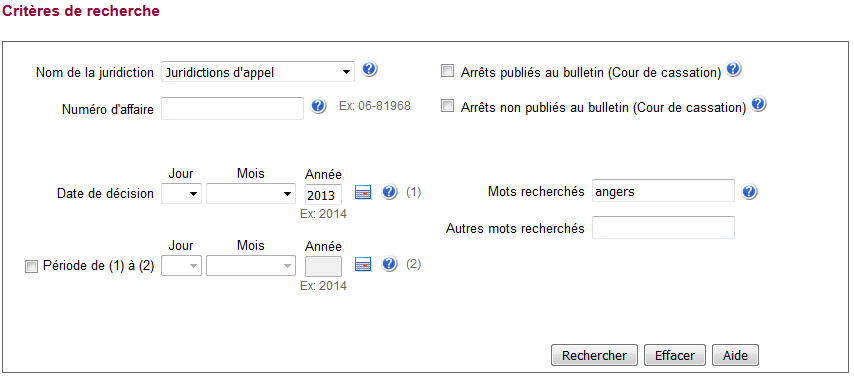
\includegraphics[width=\textwidth]{legifrance.PNG}}
		\caption{Formulaire de Légifrance}
	\end{subfigure}%

	\begin{subfigure}[t]{0.75\textwidth}
		\centering
		\fbox{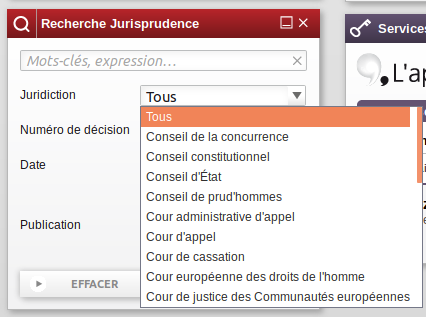
\includegraphics[width=\textwidth]{dalloz.png}}
		\caption{Formulaire de Dalloz}
	\end{subfigure}
% 	\begin{subfigure}[t]{0.56\textwidth}
% 		\centering
% 		\fbox{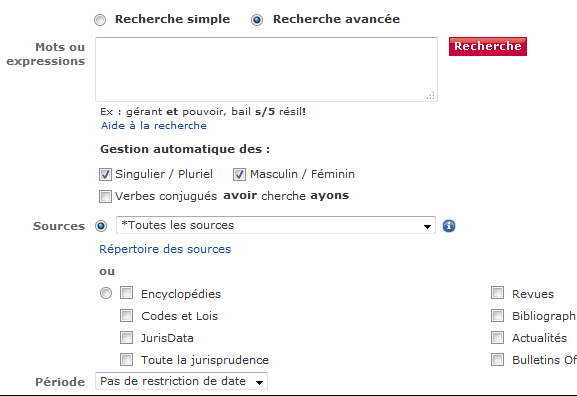
\includegraphics[width=\textwidth]{lexisnexis.png}}
% 		\caption{Formulaire de LexisNexis}
% 	\end{subfigure}%
	\caption{Exemples de critères des moteurs de recherche juridique}\label{fig:intro:juriSearchForm}
\end{figure}

Il existe aussi des moteurs de recherche juridiques qui permettent de retrouver des décisions intéressantes. Cependant, qu'ils soient payants (LexisNexis\footnote{\url{https://www.lexisnexis.fr/}}, Dalloz\footnote{\url{http://www.dalloz.fr}}, Lamyline\footnote{\url{http://lamyline.lamy.fr}},...) ou gratuits (CanLII\footnote{\url{https://www.canlii.org}}, Légifrance\footnote{\url{https://www.legifrance.gouv.fr}}, ...), les critères de recherche offerts par leurs moteurs de recherche limitent grandement la pertinence des résultats pouvant être obtenus. En effet, il ne s'agit en général que de combinaisons de mots-clés et autres méta-données (date, type de juridiction, ...), ou d'expressions régulières, comme l'illustre la \figureref{fig:intro:juriSearchForm}. La manipulation de tels critères est difficile pour constituer des échantillons pertinents suivant une sémantique souhaitée tels que l'ensemble des décisions traitant d'une catégorie de demande ou d'une circonstance factuelle donnée. 

\begin{table}[!htb]
 	\small
 	\begin{center}
 		\begin{tabular}{|l|l|l|l|l|l|}
 			\hline
 			\textbf{Justice}	& \textbf{2013}  & \textbf{2014}  & \textbf{2015}  & \textbf{2016}  & \textbf{2017}  \\ \hline
 			civile   & 2 761 554 & 2 618 374 & 2 674 878 & 2 630 085 & 2 609 394 \\ \hline
 			pénale   & 1 303 469 & 1 203 339 & 1 206 477 & 1 200 575 & 1 180 949 \\ \hline
 			administrative & 221 882 & 230 477 & 228 876 & 231 909 & 242 882 \\ \hline
 		\end{tabular}
 		
 		\textit{\scriptsize{\textbf{Source}: \url{http://www.justice.gouv.fr/statistiques-10054/chiffres-cles-de-la-justice-10303/}}}  
 	\end{center}
 	\caption{Nombre de décisions prononcées en France par an de 2013 à 2017}\label{tab:intro:nbdecisionstats}
 \end{table}
Plus de 4 millions de décisions sont prononcées en France chaque année d'après les chiffres du ministère français de la justice (\tableref{tab:intro:nbdecisionstats}). Dans ce contexte, l'analyse manuelle ne peut être limitée qu'à une infime proportion de documents disponibles.
En effet, au regard de la croissance rapide du nombre de décisions, même une étude sur une question très précise nécessite la constitution d'un large corpus de décisions pertinentes. Par ailleurs, il peut s'avérer très pénible de les lire pour en identifier les données d'intérêt. Les documents sont très souvent longs et complexes dans leur style de rédaction. Par exemple, Certaines phrases comprennent plusieurs clauses discutant d'aspects différents (\figureref{fig:intro:multiclauses}). On y retrouve aussi des références à des jugements antérieurs (\figureref{fig:intro:referencejugementanterieur}).
\begin{figure}[!htb]
\fvset{gobble=2, numbers=left, fontsize=\footnotesize}
\begin{Verbatim}[firstnumber=69]
  Exposant subir un trouble anormal de voisinage pour être privée d'une vue sur la 
  mer dont elle disposait auparavant, ce en raison de l'absence de taille de haies 
  implantées à proximité de son jardin privatif, elle a attrait devant le juge des 
  référés du tribunal de grande instance de Marseille, le syndicat des 
  copropriétaires LES CATALANS (ci-après désigné : le syndicat des copropriétaires) 
  , et son syndic recherché personnellement, le Cabinet L., à l'effet, au visa de 
  l'article 809 du code de procédure civile d'obtenir leur condamnation sous 
  astreinte de 200 euros par jour de retard à tailler les haies qui bouchent sa 
  vue et la condamnation personnelle du Cabinet L. à lui régler une provision de 
  2.000 euros à valoir sur dommages et intérêts, outre 1.500 euros sur le 
  fondement des dispositions de l'article 700 du code de procédure civile.
\end{Verbatim}
\scriptsize{\textit{\textbf{Source}: extrait de la décision R.G. 15/10226 de la Cour d'Appel d'Aix-en-Provence du 2 Juin 2016}}
  \caption{Exemple de phrases composée de plusieurs clauses dont une demande de condamnation sous astreinte, une autre de dommages et intérêts pour trouble anormal de voisinage, et une dernière de dommages et intérêts sur l'article 700 du code de procédure civile.}
  \label{fig:intro:multiclauses}
\end{figure}


\begin{figure}[!htb]
\fvset{gobble=2, numbers=left, fontsize=\footnotesize}
\begin{Verbatim}[firstnumber=73]
    Vu le jugement du tribunal de grande instance de Versailles du 5 décembre 2013 
    qui a :
    - rejeté la demande de démolition de la construction litigieuse,
\end{Verbatim}
\begin{Verbatim}[firstnumber=118, stepnumber=2]
    ...
    SUR CE LA COUR,
\end{Verbatim}
\begin{Verbatim}[firstnumber=277, stepnumber=2]
    ...  
    PAR CES MOTIFS, 
    ...
\end{Verbatim}
\begin{Verbatim}[firstnumber=281]
    Confirme le jugement en toutes ses dispositions à l'exception de celle relative 
    au montant des dommages et intérêts ...
\end{Verbatim}
\footnotesize{\textit{\textbf{Source}: extrait de la décision R.G. 14/01640 de la Cour d'Appel de Versaille du 7 Avril 2016}}
  \caption{Exemple de référence à un jugement antérieur dans une décision d'appel.}
  \label{fig:intro:referencejugementanterieur}
\end{figure}
Il est évident qu'une automatisation du traitement des corpus de décisions s'impose pour répondre aux diverses difficultés d'accès, de volumétrie, et de complexité liées à la compréhension des décisions. Une telle automatisation ferait gagner du temps aux juristes lors de tâches d'analyse métier préalables à leur raisonnement d'experts, tout en leur fournissant une vue exhaustive de la jurisprudence. D'autre part, \citet{cretin2014justicecomplexe} fait remarquer que la justice est complexe dans son organisation (\figureref{orgjusticefrance}) et son fonctionnement, et que son langage est peu compréhensible. Il est donc presque impossible pour les profanes en droit d'estimer leurs droits et le risque judiciaire qu'ils encourent dans leur quotidien sans consulter un initié du droit. L'exigence pour le profane étant l'exacte pertinence des ressources, leur accessibilité, et l'intuitivité du processus de leur exploitation \citep{narazenko2017legalnlpintro}, l'automatisation de l'analyse de la jurisprudence pourrait ainsi améliorer l'accessibilité du droit dans d'indénombrables situations. Par exemple, en comparant le montant qu'on peut espérer d'une juridiction et le coût d'un procès, on peut plus aisément se décider entre un arrangement à l'amiable et la poursuite du litige en justice \citep{langlaischappe2009ecoresolutionlitige}. Le traitement automatique de la jurisprudence constituerait alors une aide précieuse non seulement pour les professionnels du droit, mais aussi pour les particuliers et entreprises tous soucieux de voir l'issue de leur affaire leur être favorable.  

\begin{figure}[!htb]
	\centering 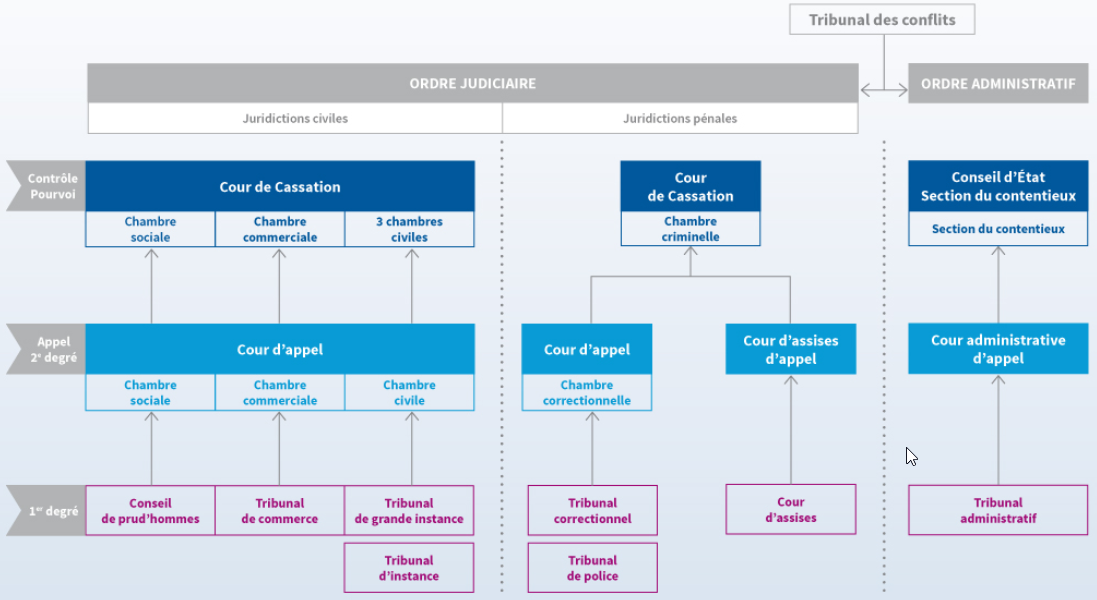
\includegraphics[angle=90,width=0.65\textwidth]{organisation_justice_francaise_grand.png}
	
	\textit{\scriptsize{\textbf{Source}: \url{http://www.justice.gouv.fr/organisation-de-la-justice-10031/}}}  
	\caption{Organisation des institutions judiciaires françaises} \label{orgjusticefrance}
\end{figure}

\section{Objectifs}
%\textcolor{red}{Description d'une approche traditionnelle, exemple d'études, difficultés de ces études}
 Ce mémoire propose des approches pour automatiser l'extraction de connaissances judiciaires à partir des décisions françaises. Le but est de faciliter la structuration et l'analyse descriptive et prédictive de corpus de décisions de justice en adressant les difficultés de l'approche traditionnelle d'analyse de contentieux. L'étude de la jurisprudence pour un contentieux donnée consiste à \citep{ancel2003expulsion} :
 \begin{enumerate}
 	\item \textbf{Choisir un échantillon représentatif}: Des décisions sont collectionnées suivant des contraintes définies:  période précise, couverture géographique, types d'affaires, etc.
 	\item \textbf{Sélectionner les décisions}: élimination des décisions qui ne correspondent pas au type de demande d'intérêt.
 	\item \textbf{Élaborer la grille d'analyse}: Un modèle de grille est créé et permet d'enregistrer les informations potentiellement importantes. Chaque ligne de la grille correspond à une demande, et les colonnes font référence aux différents types d'informations qu'il est possible d'extraire sur une demande. Ces variables vont de la procédure suivie, aux solutions proposées, en passant par la nature de l'affaire. Les champs à remplir ne sont pas connus à l'avance ; ce n'est généralement qu'au cours de la lecture des décisions que l'on distingue les informations pertinentes pour l'étude.
 	\item \textbf{L'analyse des décisions et l'interprétation des informations}: Les informations retrouvées dans les décisions sont saisies dans la grille, et des calculs statistiques sont effectués par la suite.
 \end{enumerate}
 
\citet{ancel2003expulsion} évoque principalement le problème de la différence entre l'état capté de la jurisprudence et son état présent. En effet, les longs délais de travail sont caractéristiques de ces études. L'étude de son équipe portait sur les décisions d'expulsion d'occupants sans droit ni titre. La saisie des informations à elle seule a duré 9 mois.  De plus, il est difficile d'observer l'évolution des pratiques judiciaires dans le temps et leur différence entre les villes du fait de la faible taille de l'échantillon choisi. Par exemple, \citet{jeandidier2006pensions} n'ont analysé que 399 dossiers d'affaires de pension alimentaire correspondant aux audiences s'étalant de fin 1999 à fin 2000 d'un seul tribunal de grande instance. L'équipe de \citet{ancel2003expulsion} n'a quant à elle analysé que 3865 décisions sélectionnées parmi 5656 décisions rendues du 1$^\text{er}$  juillet au 31 décembre 2001. 
 
La problématique de notre étude est \og \textbf{comment donner accès à l'analyse automatique de la sémantique d'un corpus jurisprudentiel pour comprendre la prise de décision des juges?} \fg{}. La complexité de cette analyse s'explique notamment par l'interprétation subjective des règles juridiques, l'application non déterministe de la loi, et la technicité du langage judiciaire. Cette problématique intéresse des entreprises telles que LexisNexis \footnote{\url{https://lexmachina.com}} et Lexbase SA\footnote{\url{https://www.legalmetrics.fr}}, et plusieurs startups  telles que Predictice\footnote{\url{http://predictice.com}} et CASE LAW ANALYTICS\footnote{\url{http://caselawanalytics.com}}. Afin d'y répondre, nous nous intéressons aux concepts d'informations mentionnées dans les décisions, au centre desquels se trouvent les demandes des parties (prétentions) sur lesquelles portent les conclusions rendues. Ainsi, l'analyse sémantique d'un corpus jurisprudentiel vise l'identification de connaissances sur les demandes (\figureref{fig:intro:demande-central}).
 \begin{figure}[!htb]
 	\centering
 	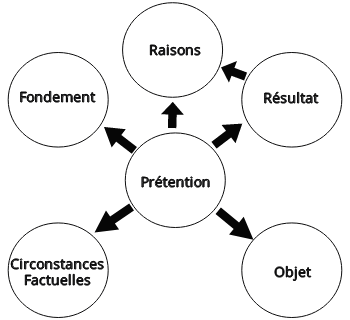
\includegraphics[scale=0.7]{demande-central.png}
 	
 	\scriptsize{\textit{Sens des flèches: l'extrémité est l'information sur l'origine.}}
 	\caption{La demande au centre de la compréhension des décisions}
 	\label{fig:intro:demande-central}
 \end{figure} 

Une demande peut être caractérisée par :
 \begin{itemize}
 	\item l'objet qui a été demandé (par ex. dommages et intérêts) quantifié par un quantum ;
	\item le résultat associé qui est décrit par une polarité (\og accepte \fg{} ou \og rejette \fg{}), souvent lié à un quantum accordé, par exemple 5000 euros de dommages et intérêts ou 2 mois d'emprisonnement;
	\item le fondement ou la norme juridique qui est la règle qui légitime la prétention ou le résultat;	
	\item les circonstances factuelles définissent des types d'affaires et qui caractérisent les différentes situations dans lesquelles sont formulées les demandes d'une catégorie donnée;
	\item les divers arguments apportés par les parties pour justifier leurs requêtes  (raisons des demandes).
	\item les motivations des solutions des juges (raisons des résultats)
 \end{itemize}

Comme illustré par la  \figureref{fig:intro:objectif-these}, l'analyse sémantique identifie ou découvre différentes informations descriptives d'un corpus constitué par des décisions collectées à partir de divers moteurs de recherche juridique et des juridictions. Cette thèse s'inscrit dans un projet qui vise, entre autres, à automatiser la constitution d'une base de connaissances sur la jurisprudence française. Une telle base permettrait notamment de mener une grande variété de recherches et d'études expertes. Elle aurait aussi naturellement une importance certaine pour la définition de modèles prédictifs par exemple pour la prédiction des types de demandes à formuler et la prédiction de la solution des juges. 

\begin{figure}[!htb]
% pipeline-cassandra.pdf
	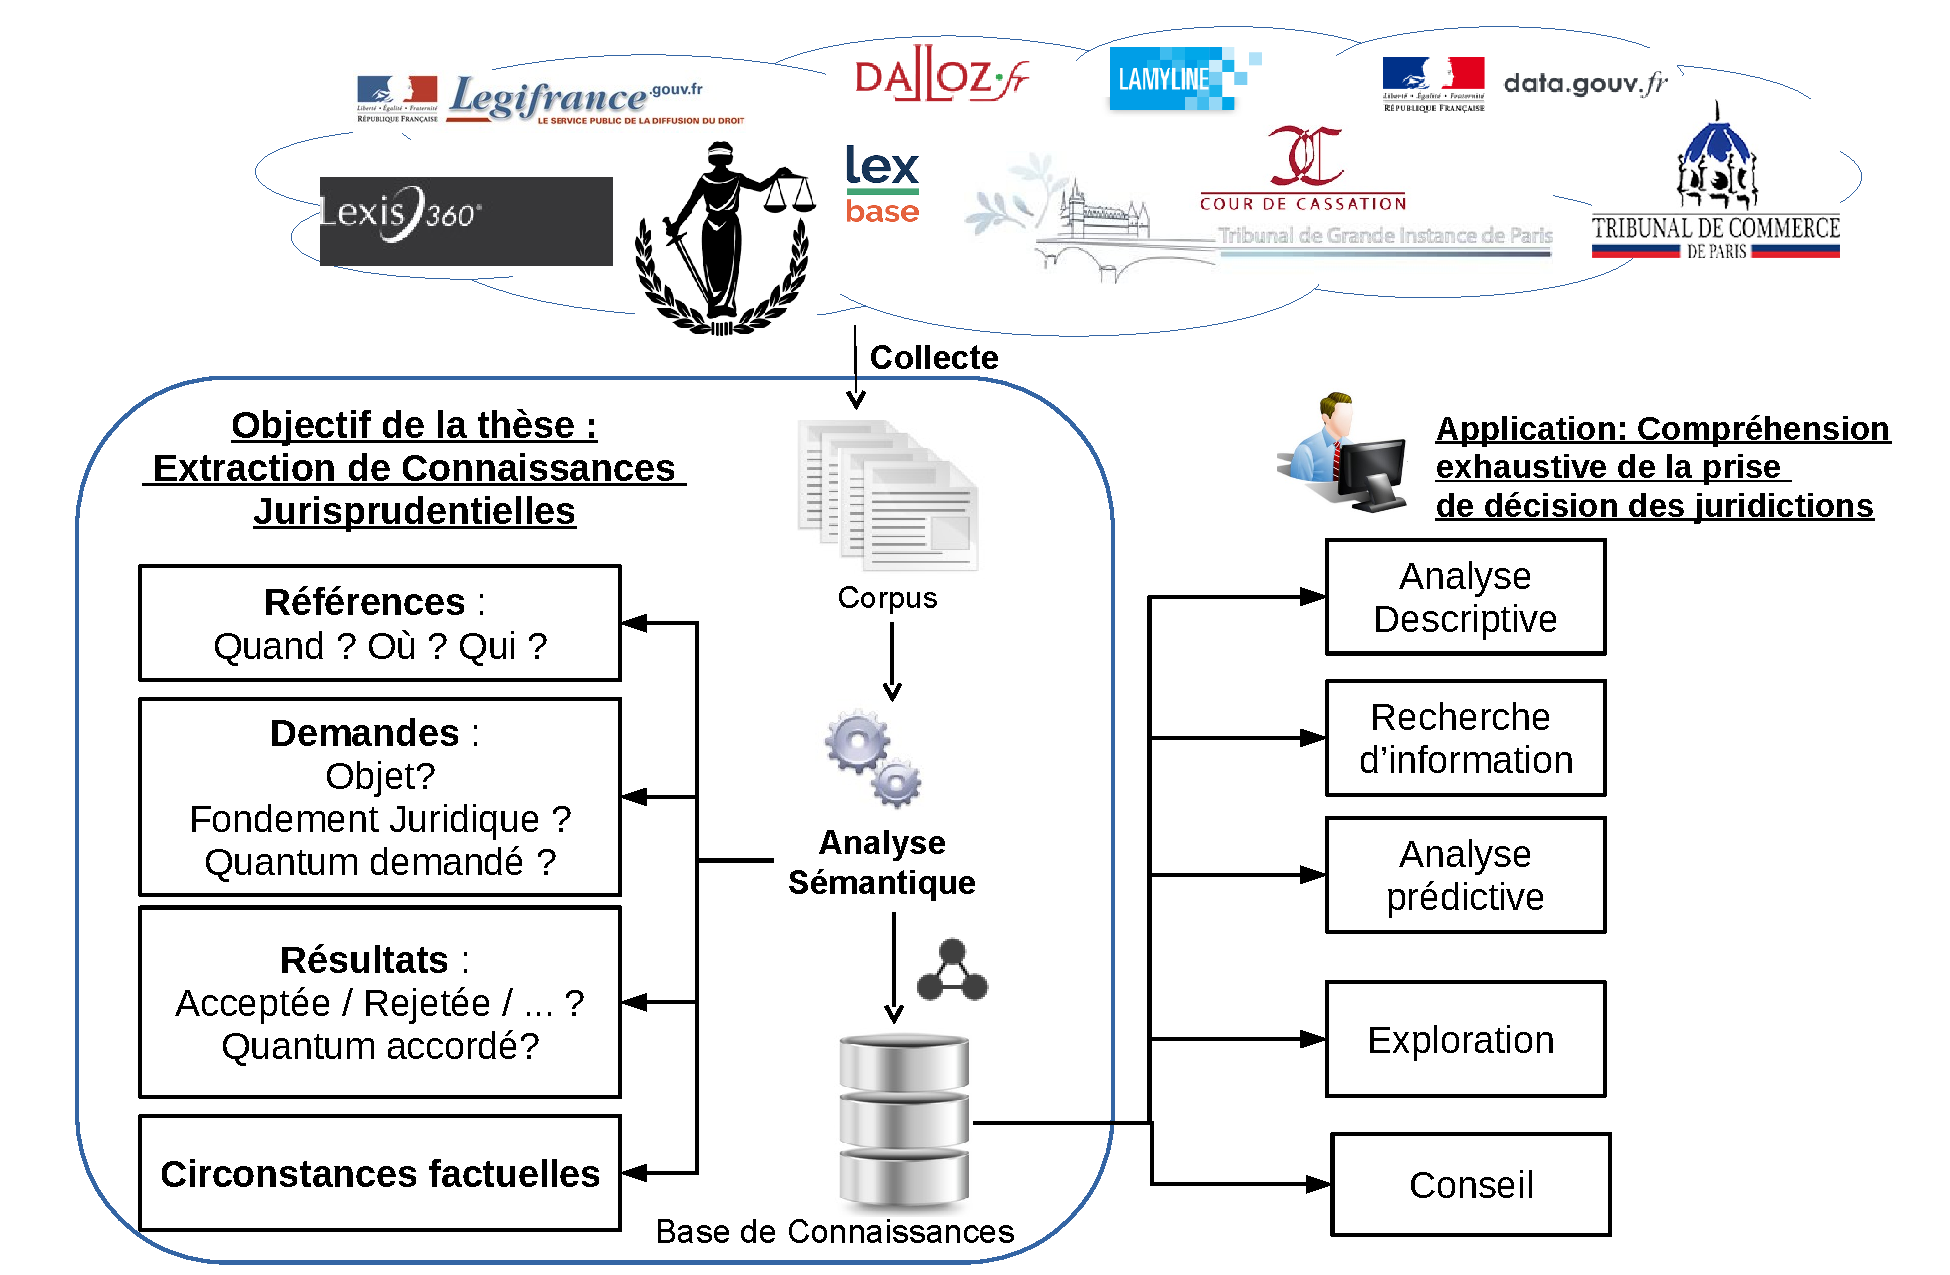
\includegraphics[width=\textwidth]{Objectif_these.pdf}
	\caption{Objectifs et applications de la thèse} \label{fig:intro:objectif-these}
\end{figure} 

\subsection{Collecte, gestion et pré-traitement des documents}
Il est nécessaire de trouver des moyens pour collecter le maximum de documents bruts non-structurés, les pré-traiter, et organiser leur gestion afin de les indexer pour faciliter leur traitement. Les décisions de cours d'appel de justice civile sont les plus accessibles à partir des moteurs de recherche juridique (Lexis360, Dalloz, LamyLine, Lexbase, Legifrance, etc.) et de la grande base de données JuriCa alimentée d'environ 180k décisions civiles par an \citep{lamanda2010}. Cependant, l'accès à ces décisions est généralement payant, et le nombre de documents simultanément téléchargeables est très faible sur les sites payants (généralement 10 à 20 décisions au maximum à la fois). La base JuriCa est la plus grosse base de décisions de cours d'appel en France. Elle est gérée par la Cour de cassation. L'accès à cette base est offert par le Service de Documentation, des Etudes et du Rapport\footnote{\url{https://www.courdecassation.fr/institution_1/composition_56/etudes_rapport_28.html}} (SDER). L'accès est payant pour les professionnels et gratuit pour les universités et centres de recherche en partenariat avec le SDER. Lexbase dispose depuis une dizaine d'année d'une licence pour vendre les décisions de JuriCa\footnote{Arrêts des cours d’appel : la base JURICA enfin en service chez Lexbase par  Emmanuel Barthe \url{https://www.precisement.org/blog/Arrets-des-cours-d-appel-la-base.html}}. Légifrance, le moteur de recherche du ministère de la justice, fournit quant à lui un accès public et gratuit à un nombre considérable de documents. Les décisions y sont identifiées à l'aide de numéros consécutifs et accessibles à partir d'un service Web. Ce dernier a l'avantage de proposer des décisions de tous les ordres et de tous les degrés. Cependant, les décisions des juridictions du premier degré (appelées jugements) restent plus rares sur internet et principalement disponibles auprès des tribunaux. Il faut préciser que nos expérimentations se sont concentrées sur les décisions d'appel en justice civile, et ce choix a été motivé par le fait qu'elles sont les plus disponibles.

%Les décisions existent sous divers formats PDF, DOC, DOCX, RTF, TXT, XML, etc. Il arrive parfois qu'un fichier téléchargé comprenne plusieurs décisions (sur LexisNexis par exemple). Nous avons par conséquent préféré convertir tous les documents au format plein texte pour homogénéiser les traitements. Par ailleurs, les décisions sont collectées à partir de diverses sources pouvant contenir des documents identiques. Il se pose donc un problème d'identification unique des décisions pour éviter des redondances. Pour cela, nous avons défini une convention de nommage des fichiers. Ce dernier repose sur 3 informations: le type de juridiction (tribunal, cour d'appel, ...), la ville, et le numéro R.G. (registre général) qui est l'identifiant unique de la décision au sein de la juridiction. Par exemple, le numéro \og CAREN1606137 \fg{} identifie la décision de numéro R.G. \og 16/06137 \fg{} de la cour d'appel (\og CA \fg{}) de la ville de Rennes (\og REN \fg{}). Ces 3 informations sont présentes dans les premières lignes de la décision, et sont facilement identifiables à l'aide d'une routine à base de règles simples. D'autre part, certains moteurs de recherche ne fournissent souvent qu'un résumé au lieu du contenu original des décisions. Il est important de supprimer ces fichiers du corpus.

\subsection{Extraction de connaissances}
\label{subsec:intro:ie}
%Les problématiques d'extraction de connaissances constituent la pierre angulaire de cette thèse car les informations sur les demandes, les parties, les juges, les juridictions et les faits conditionnent la qualité des prévisions du sens du résultat pour un type de demandes considéré.  
La difficulté d'extraire de telles informations découlent de l'état non-structuré des documents, et de la complexité et la spécificité du langage employé. L'extraction des connaissances nécessite de mettre en \oe uvre des techniques de fouille de textes adaptées à la nature des éléments à identifier. Nous avons ainsi abordé l'annotation des références de l'affaire (juridiction, ville, participants, juges, date, numéro R.G., normes citées, ...), l'extraction des demandes et résultats correspondants, et l'identification des circonstances factuelles.

Les méta-données de référence sont des segments de texte qu'on peut directement localiser dans le document. Elles sont donc semblables aux entités nommées dont la reconnaissance est une problématique intensivement étudiée en traitement automatique du langage naturel \citep{yadav2018surveyNeuralNER} dans plusieurs travaux et compétitions, aussi bien pour des entités communes \citep{tjong2003introCoNLL,grishman1996muc6}, que pour des entités spécifiques à un domaine \citep{kim2004bioNer, persson2012nbbioner,hanisch2005prominer}, et dans diverses langues \citep{li2018wcpbioner,alfred2014malayner,amarappa2015kannada}. 

Le problème d'identification des demandes consiste à reconnaître, dans la décision analysée, l'objet, le fondement, le quantum demandé, le sens du résultat correspondant, et le quantum accordé de chaque prétention. La demande s'apparente donc aux entités structurées telles que les évènements \cite{ace2005event} qui sont décrits par un type, un terme-clé, des participants, un temps, une polarité.

Le problème d'identification des circonstances factuelles consiste à constituer des regroupements de décisions mentionnant une certaine catégorie de demande (objet+fondement). Le but est, comme indiqué précédemment, de repérer les différentes situations dans lesquelles cette catégorie de demande est formulée. Chacun des groupes représente donc une situation particulière partagée par les membres du groupe mais bien distinctes de celles reflétées par les autres groupes. Ce problème évoque des problématiques de similarité entre textes, de catégorisation non-supervisée (\textit{clustering}), et de \og modélisation thématique \fg{} (\textit{topic modeling}). 

A l'issue du processus d'extraction, les données extraites sont destinées à enrichir progressivement une base de connaissances. La structuration des données au sein d'une base facilite les diverses analyses automatiques applicables aux décisions et demandes judiciaires. 

\subsection{Analyse descriptive}
L'analyse descriptive exploite l'ensemble des connaissances extraites et organisées pour répondre aux diverses questions que l'on pourrait se poser sur l'application de la loi. Il est intéressant par exemple de comparer les fréquences de résultats positifs et négatifs pour une catégorie de prétention donnée dans une situation précise. Les quanta extraits servent à visualiser les différences entre les montants accordés et réclamés. D'autres analyses plus complexes permettraient d'étudier l'évolution dans le temps et les différences dans l'espace de l'opinion des juges.


\section{Méthodologie}
\label{sec:intro:methodologie}
Les tâches sont définies par le métier.
Comme illustrées précédemment (\ref{subsec:intro:ie}), les problématiques propres aux textes juridiques trouvent généralement des analogies avec les problèmes d'analyse de données textuelles (\textit{text mining}). Ainsi, les méthodes issues de ce domaine sont applicables aux textes juridiques. Cependant, quelques adaptations sont généralement nécessaires pour obtenir des résultats de bonne qualité hors des domaines pour lesquels ces approches ont été développées \citep{Waltl2016lexia}. De plus, la recherche en fouille de textes est souvent réalisée sur des échantillons qui ne reflètent pas toujours la complexité des données réelles. Effectuant l'une des premières études d'analyse sémantique des décisions françaises, nous avons axé notre travail sur le rapprochement des problèmes liés à l'analyse des décisions jurisprudentielles de ceux généralement traités en analyse de textes. Il s'agit ensuite d'établir des protocoles d'évaluation et d'annotation manuelle de données. Selon les problématiques identifiées et les protocoles d'évaluations définis, des méthodes adaptées ont été proposées et expérimentées sur les données réelles annotées manuellement par un expert juriste.

\section{Résultats}
\label{sec:intro:résultats}
Une chaîne de traitement pour le sectionnement et l'annotation des méta-données est proposée. Premièrement, le sectionnement a pour but d'organiser l'extraction des informations qui sont réparties dans des sections selon leur nature. L'applicabilité de deux modèles probabilistes, les champs aléatoires conditionnels ou CRF (\textit{conditional random fields}) et les modèles cachés de Markov ou HMM (\textit{hidden Markov Model}), est étudiée en considérant plusieurs aspects de la conception des systèmes d'extraction d'entités nommées.  

Par la suite, nous proposons une méthode d'extraction des demandes et des résultats en fonction des catégories présentes dans la décision. L'approche consiste en effet à identifier dans un premier temps les catégories (objet+fondement) présentes par classification supervisée. Un vocabulaire d'expression des demandes et résultats est exploité pour identifier les passages. Puis à l'aide de termes propres à chacune des catégories identifiées, les trois attributs (quantum demandé, sens du résultat, quantum accordé) des paires demande-résultat sont reconnus. 

Par ailleurs, nous analysons l'extraction du sens du résultat par classification binaire des documents. L'objectif est de s'affranchir de l'identification préalable de l'expression des demandes et résultats. En effet, les décisions comprenant des demandes d'une catégorie donnée semblent ne contenir, dans une forte proportion, qu'une seule demande. %Nous pensons qu'il n'est par conséquent pas nécessaire d'identifier l'expression de cette dernière pour en déterminer le sens. 
A partir d'une représentation adéquate du contenu de la décision, il est possible de classer cette dernière à l'aide d'un modèle de classification supervisée de documents.

L'identification des circonstances factuelles, quant à elle, est modélisée comme une tâche de regroupement non supervisé de documents. Nous proposons dans ce cas une méthode d'apprentissage d'une distance entre textes, à l'aide d'un algorithme de régression. La métrique apprise est utilisée dans l'algorithme des \og K-moyennes \fg{} (\textit{k-means}) \citep{forgey1965kmeans} et celui des \og K-medoïdes \fg{} (\textit{k-medoids}) \citep{kaufman1987kmedoids}, et comparée à d'autres distances établies en recherche d'information.

\section{Structure de la thèse}
\label{sec:intro:organisation}

La thèse est organisée en 6 chapitres. Le chapitre \ref{chap:literature} positionne nos travaux par rapport à ceux qui ont été réalisés précédemment sur des problématiques d'analyse automatique de décisions de justice. Le chapitre \ref{chap:structuration} présente les architectures et modèles proposés pour la structuration des décisions et la reconnaissance des entités juridiques ; il discute notamment des différents résultats empiriques obtenus par application des modèles CRF et HMM. Ensuite, le chapitre \ref{chap:quanta} détaille le problème  d'extraction des demandes, puis présente notre méthode et les résultats obtenus. Le chapitre \ref{chap:sensresultat} traite de l'identification du sens du résultat par classification directe des décisions, cela en comparant différents algorithmes de classification et de représentations des textes. Le chapitre \ref{chap:similarite} discute de l'usage de l'apprentissage proposé d'une distance qui est comparée à d'autres distances pour la découverte des circonstances factuelles. Enfin, le chapitre \ref{chap:demo} présente des résultats de scénarios d'analyses descriptives pour illustrer l'exploitation potentielle de nos propositions sur un corpus de grande taille. 

\chapter*{Introduction générale}
\label{chap:intro}
\addcontentsline{toc}{chapter}{\nameref{chap:intro}}

\section{Contexte et motivations}
\label{sec:intro:contexte}
Une décision judiciaire peut être définie soit comme  le résultat rendu par les juges à l'issue d'un procès, soit comme un document décrivant une affaire judiciaire. Un tel document rapporte, notamment,  les faits, les procédures judiciaires antérieures, le verdict des juges, et les explications associées. Dans cette thèse, nous désignons par \og décision \fg{} le document, et par  \og résultat\fg{} une conclusion ou réponse des juges. Une jurisprudence
%\footnote{\url{http://www.toupie.org/Dictionnaire/Jurisprudence.htm}} 
est un ensemble de décisions rendues par les tribunaux. Elle représente la manière dont ces derniers interprètent les lois pour résoudre un problème juridique donné (type de contentieux). Les juristes doivent alors collecter des décisions traitant de situations similaires, les sélectionner, et les analyser afin de mener, par exemple, des recherches empiriques en droit \citep{ancel2003expulsion, jeandidier2006pensions}. Les avocats exploitent aussi les décisions passées pour anticiper les résultats des juges. Ils peuvent ainsi mieux conseiller leurs clients sur le risque judiciaire que ces derniers encourent, et sur la stratégie à adopter pour faire accepter leurs demandes et faire rejeter celles de leurs adversaires. Cette activité de collecte et d'analyse, centrale pour de nombreux métiers du droit, est généralement effectuée manuellement. Elle est par conséquent sujette à plusieurs difficultés liées à l'accès et à l'exhaustivité des documents traités même lors de l'étude d'une question spécifique. Il faut notamment souligner ici que les documents sont dispersés dans les nombreux tribunaux, et que les procédures administratives ne facilitent pas toujours leur accès du fait de la nécessité de préserver la confidentialité des parties. En effet, les décisions n'étant pas \og anonymisées \fg{} la plupart du temps, elles restent alors inaccessibles aux juristes qui en font la demande. Un certain nombre de documents sont néanmoins accessibles sur internet grâce à des sites de publication de données ouvertes gouvernementales\footnote{Données ouvertes gouvernementales: \hyperlink{http://data.gouv.fr}{data.gouv.fr} en France, \hyperlink{https://www.judiciary.uk}{judiciary.uk} en Grande-Bretagne, \hyperlink{http://www.scotusblog.com/}{scotusblog.com} aux Etats-Unis, et \hyperlink{https://www.scc-csc.ca/}{scc-csc.ca} au Canada.}. Ces sites publient régulièrement des décisions récemment prononcées. 

\begin{figure}[!htb]
	\centering
	\begin{subfigure}[t]{\textwidth}
		\centering
		\fbox{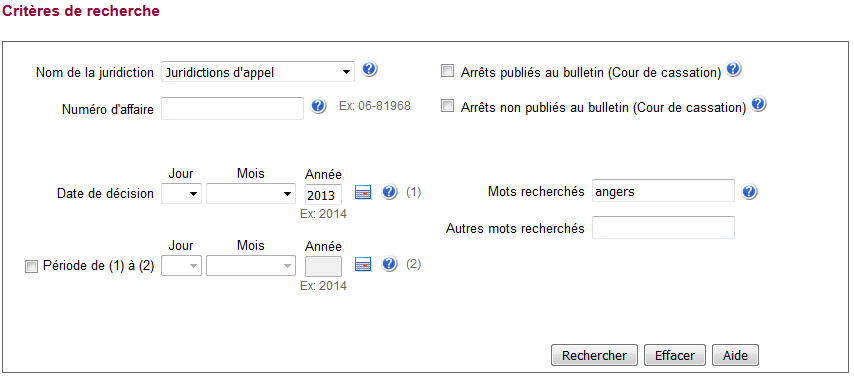
\includegraphics[width=\textwidth]{legifrance.PNG}}
		\caption{Formulaire de Légifrance}
	\end{subfigure}%

	\begin{subfigure}[t]{0.75\textwidth}
		\centering
		\fbox{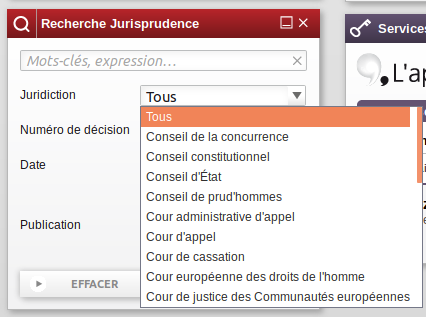
\includegraphics[width=\textwidth]{dalloz.png}}
		\caption{Formulaire de Dalloz}
	\end{subfigure}
% 	\begin{subfigure}[t]{0.56\textwidth}
% 		\centering
% 		\fbox{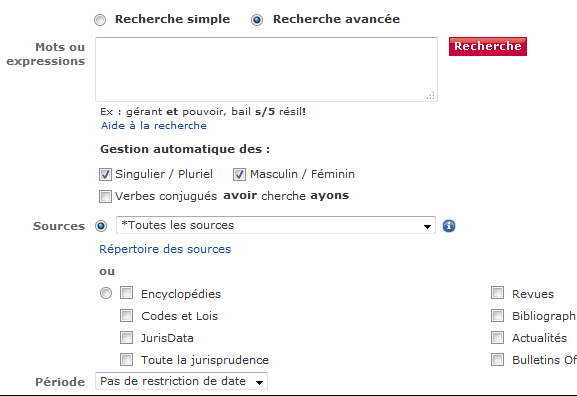
\includegraphics[width=\textwidth]{lexisnexis.png}}
% 		\caption{Formulaire de LexisNexis}
% 	\end{subfigure}%
	\caption{Exemples de critères des moteurs de recherche juridique}\label{fig:intro:juriSearchForm}
\end{figure}

Il existe aussi des moteurs de recherche juridiques qui permettent de retrouver des décisions intéressantes. Cependant, qu'ils soient payants (LexisNexis\footnote{\url{https://www.lexisnexis.fr/}}, Dalloz\footnote{\url{http://www.dalloz.fr}}, Lamyline\footnote{\url{http://lamyline.lamy.fr}},...) ou gratuits (CanLII\footnote{\url{https://www.canlii.org}}, Légifrance\footnote{\url{https://www.legifrance.gouv.fr}}, ...), les critères de recherche offerts par leurs moteurs de recherche limitent grandement la pertinence des résultats pouvant être obtenus. En effet, il ne s'agit en général que de combinaisons de mots-clés et autres méta-données (date, type de juridiction, ...), ou d'expressions régulières, comme l'illustre la \figureref{fig:intro:juriSearchForm}. La manipulation de tels critères est difficile pour constituer des échantillons pertinents suivant une sémantique souhaitée tels que l'ensemble des décisions traitant d'une catégorie de demande ou d'une circonstance factuelle donnée. 

\begin{table}[!htb]
 	\small
 	\begin{center}
 		\begin{tabular}{|l|l|l|l|l|l|}
 			\hline
 			\textbf{Justice}	& \textbf{2013}  & \textbf{2014}  & \textbf{2015}  & \textbf{2016}  & \textbf{2017}  \\ \hline
 			civile   & 2 761 554 & 2 618 374 & 2 674 878 & 2 630 085 & 2 609 394 \\ \hline
 			pénale   & 1 303 469 & 1 203 339 & 1 206 477 & 1 200 575 & 1 180 949 \\ \hline
 			administrative & 221 882 & 230 477 & 228 876 & 231 909 & 242 882 \\ \hline
 		\end{tabular}
 		
 		\textit{\scriptsize{\textbf{Source}: \url{http://www.justice.gouv.fr/statistiques-10054/chiffres-cles-de-la-justice-10303/}}}  
 	\end{center}
 	\caption{Nombre de décisions prononcées en France par an de 2013 à 2017}\label{tab:intro:nbdecisionstats}
 \end{table}
Plus de 4 millions de décisions sont prononcées en France chaque année d'après les chiffres du ministère français de la justice (\tableref{tab:intro:nbdecisionstats}). Dans ce contexte, l'analyse manuelle ne peut être limitée qu'à une infime proportion de documents disponibles.
En effet, au regard de la croissance rapide du nombre de décisions, même une étude sur une question très précise nécessite la constitution d'un large corpus de décisions pertinentes. Par ailleurs, il peut s'avérer très pénible de les lire pour en identifier les données d'intérêt. Les documents sont très souvent longs et complexes dans leur style de rédaction. Par exemple, Certaines phrases comprennent plusieurs clauses discutant d'aspects différents (\figureref{fig:intro:multiclauses}). On y retrouve aussi des références à des jugements antérieurs (\figureref{fig:intro:referencejugementanterieur}).
\begin{figure}[!htb]
\fvset{gobble=2, numbers=left, fontsize=\footnotesize}
\begin{Verbatim}[firstnumber=69]
  Exposant subir un trouble anormal de voisinage pour être privée d'une vue sur la 
  mer dont elle disposait auparavant, ce en raison de l'absence de taille de haies 
  implantées à proximité de son jardin privatif, elle a attrait devant le juge des 
  référés du tribunal de grande instance de Marseille, le syndicat des 
  copropriétaires LES CATALANS (ci-après désigné : le syndicat des copropriétaires) 
  , et son syndic recherché personnellement, le Cabinet L., à l'effet, au visa de 
  l'article 809 du code de procédure civile d'obtenir leur condamnation sous 
  astreinte de 200 euros par jour de retard à tailler les haies qui bouchent sa 
  vue et la condamnation personnelle du Cabinet L. à lui régler une provision de 
  2.000 euros à valoir sur dommages et intérêts, outre 1.500 euros sur le 
  fondement des dispositions de l'article 700 du code de procédure civile.
\end{Verbatim}
\scriptsize{\textit{\textbf{Source}: extrait de la décision R.G. 15/10226 de la Cour d'Appel d'Aix-en-Provence du 2 Juin 2016}}
  \caption{Exemple de phrases composée de plusieurs clauses dont une demande de condamnation sous astreinte, une autre de dommages et intérêts pour trouble anormal de voisinage, et une dernière de dommages et intérêts sur l'article 700 du code de procédure civile.}
  \label{fig:intro:multiclauses}
\end{figure}


\begin{figure}[!htb]
\fvset{gobble=2, numbers=left, fontsize=\footnotesize}
\begin{Verbatim}[firstnumber=73]
    Vu le jugement du tribunal de grande instance de Versailles du 5 décembre 2013 
    qui a :
    - rejeté la demande de démolition de la construction litigieuse,
\end{Verbatim}
\begin{Verbatim}[firstnumber=118, stepnumber=2]
    ...
    SUR CE LA COUR,
\end{Verbatim}
\begin{Verbatim}[firstnumber=277, stepnumber=2]
    ...  
    PAR CES MOTIFS, 
    ...
\end{Verbatim}
\begin{Verbatim}[firstnumber=281]
    Confirme le jugement en toutes ses dispositions à l'exception de celle relative 
    au montant des dommages et intérêts ...
\end{Verbatim}
\footnotesize{\textit{\textbf{Source}: extrait de la décision R.G. 14/01640 de la Cour d'Appel de Versaille du 7 Avril 2016}}
  \caption{Exemple de référence à un jugement antérieur dans une décision d'appel.}
  \label{fig:intro:referencejugementanterieur}
\end{figure}
Il est évident qu'une automatisation du traitement des corpus de décisions s'impose pour répondre aux diverses difficultés d'accès, de volumétrie, et de complexité liées à la compréhension des décisions. Une telle automatisation ferait gagner du temps aux juristes lors de tâches d'analyse métier préalables à leur raisonnement d'experts, tout en leur fournissant une vue exhaustive de la jurisprudence. D'autre part, \citet{cretin2014justicecomplexe} fait remarquer que la justice est complexe dans son organisation (\figureref{orgjusticefrance}) et son fonctionnement, et que son langage est peu compréhensible. Il est donc presque impossible pour les profanes en droit d'estimer leurs droits et le risque judiciaire qu'ils encourent dans leur quotidien sans consulter un initié du droit. L'exigence pour le profane étant l'exacte pertinence des ressources, leur accessibilité, et l'intuitivité du processus de leur exploitation \citep{narazenko2017legalnlpintro}, l'automatisation de l'analyse de la jurisprudence pourrait ainsi améliorer l'accessibilité du droit dans d'indénombrables situations. Par exemple, en comparant le montant qu'on peut espérer d'une juridiction et le coût d'un procès, on peut plus aisément se décider entre un arrangement à l'amiable et la poursuite du litige en justice \citep{langlaischappe2009ecoresolutionlitige}. Le traitement automatique de la jurisprudence constituerait alors une aide précieuse non seulement pour les professionnels du droit, mais aussi pour les particuliers et entreprises tous soucieux de voir l'issue de leur affaire leur être favorable.  

\begin{figure}[!htb]
	\centering 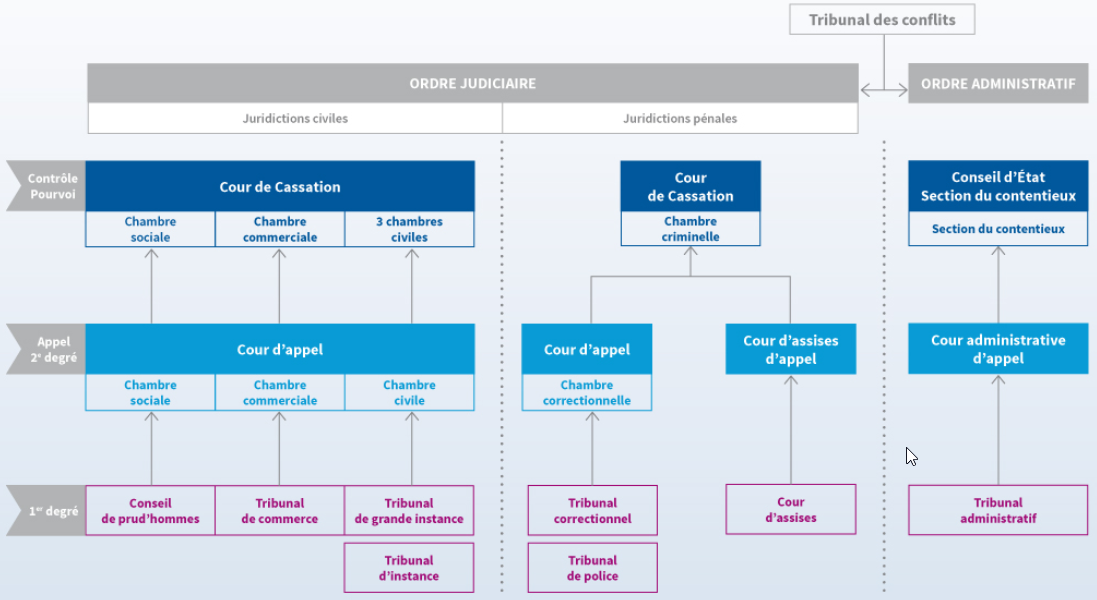
\includegraphics[angle=90,width=0.65\textwidth]{organisation_justice_francaise_grand.png}
	
	\textit{\scriptsize{\textbf{Source}: \url{http://www.justice.gouv.fr/organisation-de-la-justice-10031/}}}  
	\caption{Organisation des institutions judiciaires françaises} \label{orgjusticefrance}
\end{figure}

\section{Objectifs}
%\textcolor{red}{Description d'une approche traditionnelle, exemple d'études, difficultés de ces études}
 Ce mémoire propose des approches pour automatiser l'extraction de connaissances judiciaires à partir des décisions françaises. Le but est de faciliter la structuration et l'analyse descriptive et prédictive de corpus de décisions de justice en adressant les difficultés de l'approche traditionnelle d'analyse de contentieux. L'étude de la jurisprudence pour un contentieux donnée consiste à \citep{ancel2003expulsion} :
 \begin{enumerate}
 	\item \textbf{Choisir un échantillon représentatif}: Des décisions sont collectionnées suivant des contraintes définies:  période précise, couverture géographique, types d'affaires, etc.
 	\item \textbf{Sélectionner les décisions}: élimination des décisions qui ne correspondent pas au type de demande d'intérêt.
 	\item \textbf{Élaborer la grille d'analyse}: Un modèle de grille est créé et permet d'enregistrer les informations potentiellement importantes. Chaque ligne de la grille correspond à une demande, et les colonnes font référence aux différents types d'informations qu'il est possible d'extraire sur une demande. Ces variables vont de la procédure suivie, aux solutions proposées, en passant par la nature de l'affaire. Les champs à remplir ne sont pas connus à l'avance ; ce n'est généralement qu'au cours de la lecture des décisions que l'on distingue les informations pertinentes pour l'étude.
 	\item \textbf{L'analyse des décisions et l'interprétation des informations}: Les informations retrouvées dans les décisions sont saisies dans la grille, et des calculs statistiques sont effectués par la suite.
 \end{enumerate}
 
\citet{ancel2003expulsion} évoque principalement le problème de la différence entre l'état capté de la jurisprudence et son état présent. En effet, les longs délais de travail sont caractéristiques de ces études. L'étude de son équipe portait sur les décisions d'expulsion d'occupants sans droit ni titre. La saisie des informations à elle seule a duré 9 mois.  De plus, il est difficile d'observer l'évolution des pratiques judiciaires dans le temps et leur différence entre les villes du fait de la faible taille de l'échantillon choisi. Par exemple, \citet{jeandidier2006pensions} n'ont analysé que 399 dossiers d'affaires de pension alimentaire correspondant aux audiences s'étalant de fin 1999 à fin 2000 d'un seul tribunal de grande instance. L'équipe de \citet{ancel2003expulsion} n'a quant à elle analysé que 3865 décisions sélectionnées parmi 5656 décisions rendues du 1$^\text{er}$  juillet au 31 décembre 2001. 
 
La problématique de notre étude est \og \textbf{comment donner accès à l'analyse automatique de la sémantique d'un corpus jurisprudentiel pour comprendre la prise de décision des juges?} \fg{}. La complexité de cette analyse s'explique notamment par l'interprétation subjective des règles juridiques, l'application non déterministe de la loi, et la technicité du langage judiciaire. Cette problématique intéresse des entreprises telles que LexisNexis \footnote{\url{https://lexmachina.com}} et Lexbase SA\footnote{\url{https://www.legalmetrics.fr}}, et plusieurs startups  telles que Predictice\footnote{\url{http://predictice.com}} et CASE LAW ANALYTICS\footnote{\url{http://caselawanalytics.com}}. Afin d'y répondre, nous nous intéressons aux concepts d'informations mentionnées dans les décisions, au centre desquels se trouvent les demandes des parties (prétentions) sur lesquelles portent les conclusions rendues. Ainsi, l'analyse sémantique d'un corpus jurisprudentiel vise l'identification de connaissances sur les demandes (\figureref{fig:intro:demande-central}).
 \begin{figure}[!htb]
 	\centering
 	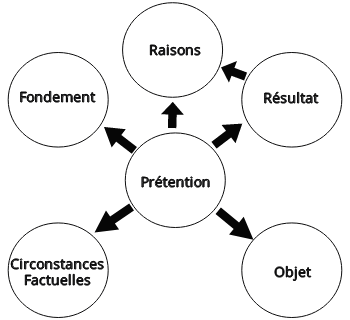
\includegraphics[scale=0.7]{demande-central.png}
 	
 	\scriptsize{\textit{Sens des flèches: l'extrémité est l'information sur l'origine.}}
 	\caption{La demande au centre de la compréhension des décisions}
 	\label{fig:intro:demande-central}
 \end{figure} 

Une demande peut être caractérisée par :
 \begin{itemize}
 	\item l'objet qui a été demandé (par ex. dommages et intérêts) quantifié par un quantum ;
	\item le résultat associé qui est décrit par une polarité (\og accepte \fg{} ou \og rejette \fg{}), souvent lié à un quantum accordé, par exemple 5000 euros de dommages et intérêts ou 2 mois d'emprisonnement;
	\item le fondement ou la norme juridique qui est la règle qui légitime la prétention ou le résultat;	
	\item les circonstances factuelles définissent des types d'affaires et qui caractérisent les différentes situations dans lesquelles sont formulées les demandes d'une catégorie donnée;
	\item les divers arguments apportés par les parties pour justifier leurs requêtes  (raisons des demandes).
	\item les motivations des solutions des juges (raisons des résultats)
 \end{itemize}

Comme illustré par la  \figureref{fig:intro:objectif-these}, l'analyse sémantique identifie ou découvre différentes informations descriptives d'un corpus constitué par des décisions collectées à partir de divers moteurs de recherche juridique et des juridictions. Cette thèse s'inscrit dans un projet qui vise, entre autres, à automatiser la constitution d'une base de connaissances sur la jurisprudence française. Une telle base permettrait notamment de mener une grande variété de recherches et d'études expertes. Elle aurait aussi naturellement une importance certaine pour la définition de modèles prédictifs par exemple pour la prédiction des types de demandes à formuler et la prédiction de la solution des juges. 

\begin{figure}[!htb]
% pipeline-cassandra.pdf
	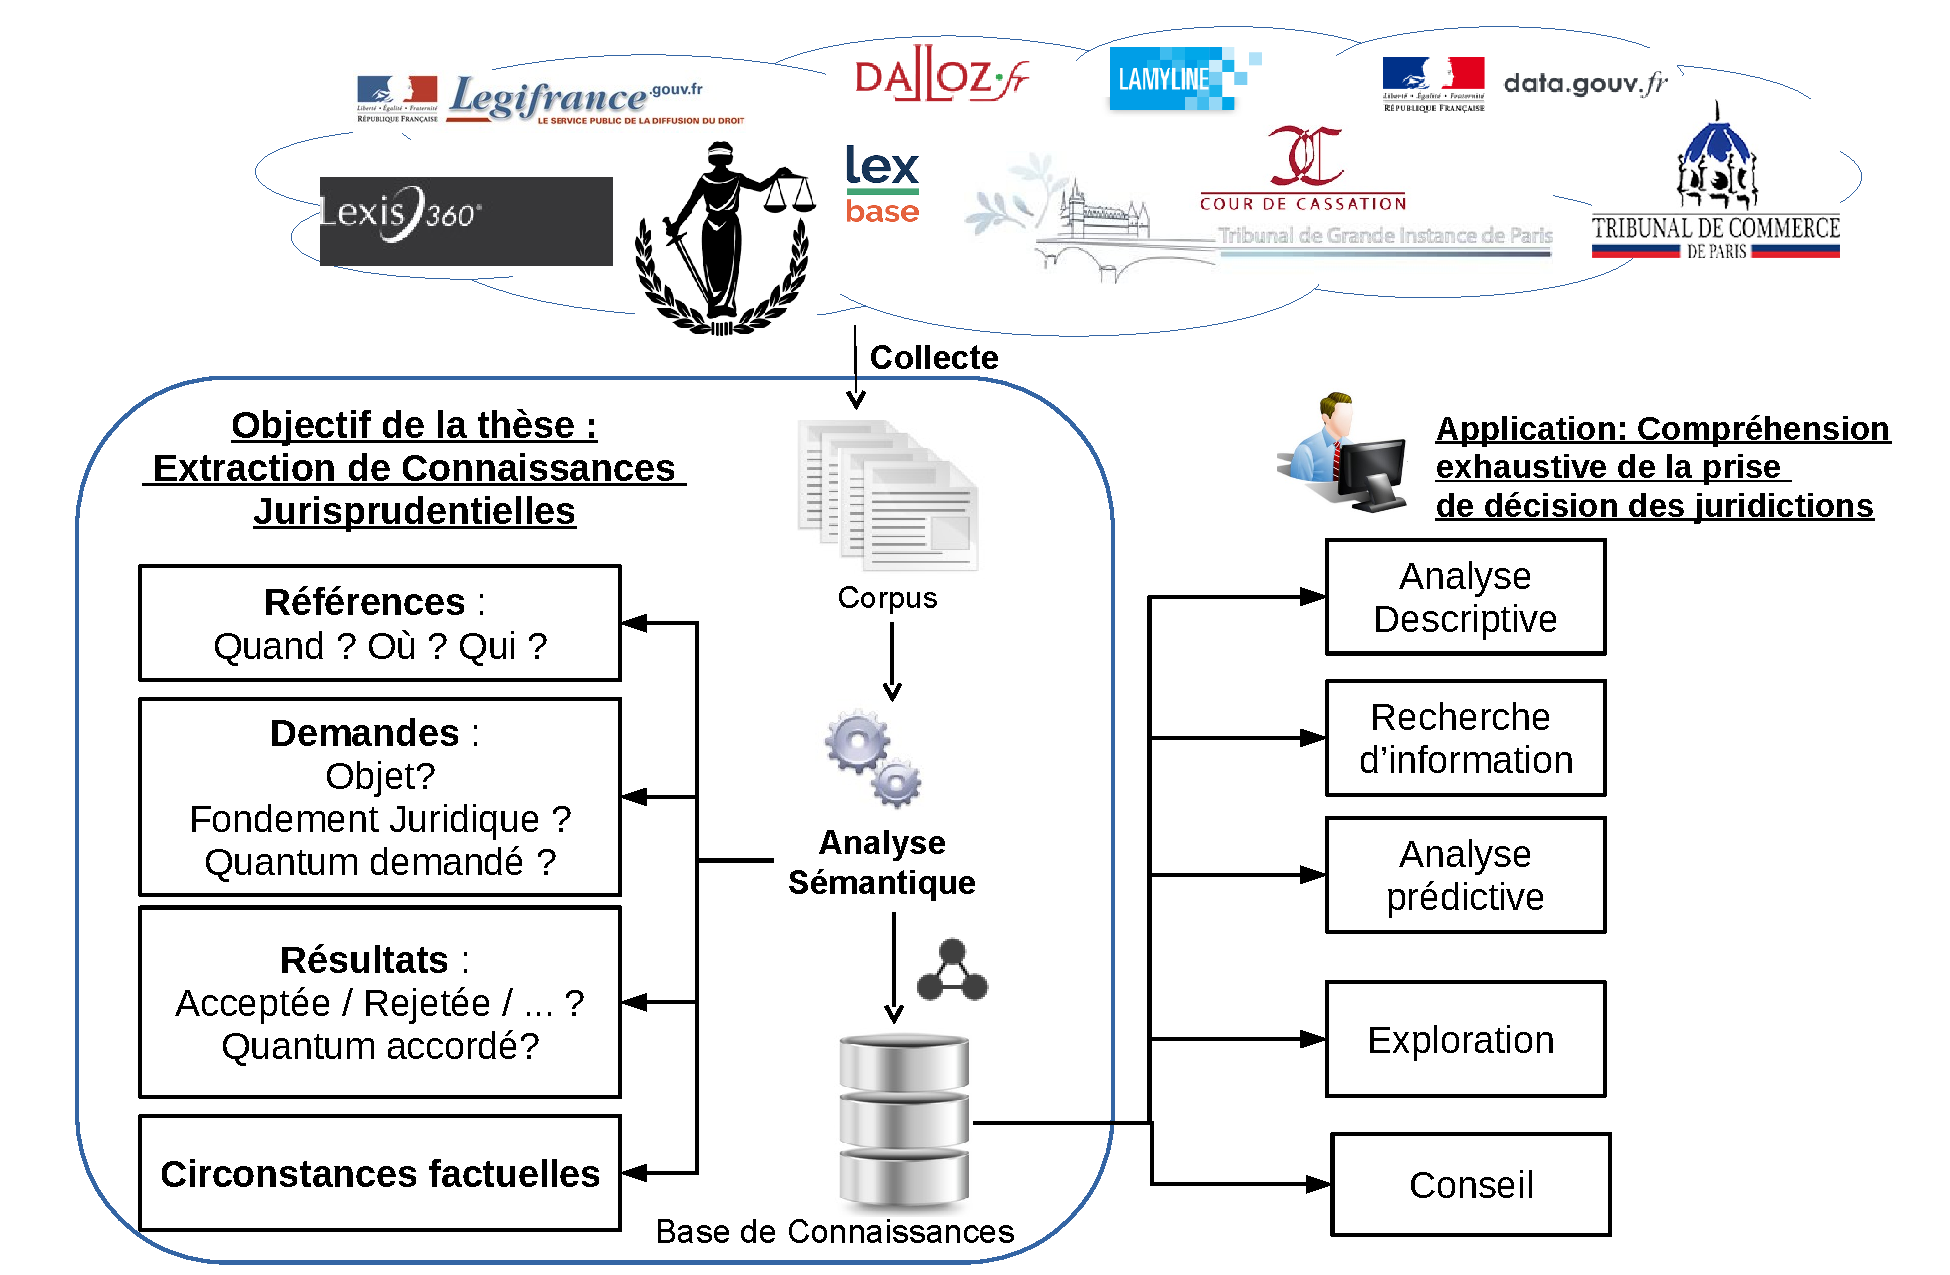
\includegraphics[width=\textwidth]{Objectif_these.pdf}
	\caption{Objectifs et applications de la thèse} \label{fig:intro:objectif-these}
\end{figure} 

\subsection{Collecte, gestion et pré-traitement des documents}
Il est nécessaire de trouver des moyens pour collecter le maximum de documents bruts non-structurés, les pré-traiter, et organiser leur gestion afin de les indexer pour faciliter leur traitement. Les décisions de cours d'appel de justice civile sont les plus accessibles à partir des moteurs de recherche juridique (Lexis360, Dalloz, LamyLine, Lexbase, Legifrance, etc.) et de la grande base de données JuriCa alimentée d'environ 180k décisions civiles par an \citep{lamanda2010}. Cependant, l'accès à ces décisions est généralement payant, et le nombre de documents simultanément téléchargeables est très faible sur les sites payants (généralement 10 à 20 décisions au maximum à la fois). La base JuriCa est la plus grosse base de décisions de cours d'appel en France. Elle est gérée par la Cour de cassation. L'accès à cette base est offert par le Service de Documentation, des Etudes et du Rapport\footnote{\url{https://www.courdecassation.fr/institution_1/composition_56/etudes_rapport_28.html}} (SDER). L'accès est payant pour les professionnels et gratuit pour les universités et centres de recherche en partenariat avec le SDER. Lexbase dispose depuis une dizaine d'année d'une licence pour vendre les décisions de JuriCa\footnote{Arrêts des cours d’appel : la base JURICA enfin en service chez Lexbase par  Emmanuel Barthe \url{https://www.precisement.org/blog/Arrets-des-cours-d-appel-la-base.html}}. Légifrance, le moteur de recherche du ministère de la justice, fournit quant à lui un accès public et gratuit à un nombre considérable de documents. Les décisions y sont identifiées à l'aide de numéros consécutifs et accessibles à partir d'un service Web. Ce dernier a l'avantage de proposer des décisions de tous les ordres et de tous les degrés. Cependant, les décisions des juridictions du premier degré (appelées jugements) restent plus rares sur internet et principalement disponibles auprès des tribunaux. Il faut préciser que nos expérimentations se sont concentrées sur les décisions d'appel en justice civile, et ce choix a été motivé par le fait qu'elles sont les plus disponibles.

%Les décisions existent sous divers formats PDF, DOC, DOCX, RTF, TXT, XML, etc. Il arrive parfois qu'un fichier téléchargé comprenne plusieurs décisions (sur LexisNexis par exemple). Nous avons par conséquent préféré convertir tous les documents au format plein texte pour homogénéiser les traitements. Par ailleurs, les décisions sont collectées à partir de diverses sources pouvant contenir des documents identiques. Il se pose donc un problème d'identification unique des décisions pour éviter des redondances. Pour cela, nous avons défini une convention de nommage des fichiers. Ce dernier repose sur 3 informations: le type de juridiction (tribunal, cour d'appel, ...), la ville, et le numéro R.G. (registre général) qui est l'identifiant unique de la décision au sein de la juridiction. Par exemple, le numéro \og CAREN1606137 \fg{} identifie la décision de numéro R.G. \og 16/06137 \fg{} de la cour d'appel (\og CA \fg{}) de la ville de Rennes (\og REN \fg{}). Ces 3 informations sont présentes dans les premières lignes de la décision, et sont facilement identifiables à l'aide d'une routine à base de règles simples. D'autre part, certains moteurs de recherche ne fournissent souvent qu'un résumé au lieu du contenu original des décisions. Il est important de supprimer ces fichiers du corpus.

\subsection{Extraction de connaissances}
\label{subsec:intro:ie}
%Les problématiques d'extraction de connaissances constituent la pierre angulaire de cette thèse car les informations sur les demandes, les parties, les juges, les juridictions et les faits conditionnent la qualité des prévisions du sens du résultat pour un type de demandes considéré.  
La difficulté d'extraire de telles informations découlent de l'état non-structuré des documents, et de la complexité et la spécificité du langage employé. L'extraction des connaissances nécessite de mettre en \oe uvre des techniques de fouille de textes adaptées à la nature des éléments à identifier. Nous avons ainsi abordé l'annotation des références de l'affaire (juridiction, ville, participants, juges, date, numéro R.G., normes citées, ...), l'extraction des demandes et résultats correspondants, et l'identification des circonstances factuelles.

Les méta-données de référence sont des segments de texte qu'on peut directement localiser dans le document. Elles sont donc semblables aux entités nommées dont la reconnaissance est une problématique intensivement étudiée en traitement automatique du langage naturel \citep{yadav2018surveyNeuralNER} dans plusieurs travaux et compétitions, aussi bien pour des entités communes \citep{tjong2003introCoNLL,grishman1996muc6}, que pour des entités spécifiques à un domaine \citep{kim2004bioNer, persson2012nbbioner,hanisch2005prominer}, et dans diverses langues \citep{li2018wcpbioner,alfred2014malayner,amarappa2015kannada}. 

Le problème d'identification des demandes consiste à reconnaître, dans la décision analysée, l'objet, le fondement, le quantum demandé, le sens du résultat correspondant, et le quantum accordé de chaque prétention. La demande s'apparente donc aux entités structurées telles que les évènements \cite{ace2005event} qui sont décrits par un type, un terme-clé, des participants, un temps, une polarité.

Le problème d'identification des circonstances factuelles consiste à constituer des regroupements de décisions mentionnant une certaine catégorie de demande (objet+fondement). Le but est, comme indiqué précédemment, de repérer les différentes situations dans lesquelles cette catégorie de demande est formulée. Chacun des groupes représente donc une situation particulière partagée par les membres du groupe mais bien distinctes de celles reflétées par les autres groupes. Ce problème évoque des problématiques de similarité entre textes, de catégorisation non-supervisée (\textit{clustering}), et de \og modélisation thématique \fg{} (\textit{topic modeling}). 

A l'issue du processus d'extraction, les données extraites sont destinées à enrichir progressivement une base de connaissances. La structuration des données au sein d'une base facilite les diverses analyses automatiques applicables aux décisions et demandes judiciaires. 

\subsection{Analyse descriptive}
L'analyse descriptive exploite l'ensemble des connaissances extraites et organisées pour répondre aux diverses questions que l'on pourrait se poser sur l'application de la loi. Il est intéressant par exemple de comparer les fréquences de résultats positifs et négatifs pour une catégorie de prétention donnée dans une situation précise. Les quanta extraits servent à visualiser les différences entre les montants accordés et réclamés. D'autres analyses plus complexes permettraient d'étudier l'évolution dans le temps et les différences dans l'espace de l'opinion des juges.


\section{Méthodologie}
\label{sec:intro:methodologie}
Les tâches sont définies par le métier.
Comme illustrées précédemment (\ref{subsec:intro:ie}), les problématiques propres aux textes juridiques trouvent généralement des analogies avec les problèmes d'analyse de données textuelles (\textit{text mining}). Ainsi, les méthodes issues de ce domaine sont applicables aux textes juridiques. Cependant, quelques adaptations sont généralement nécessaires pour obtenir des résultats de bonne qualité hors des domaines pour lesquels ces approches ont été développées \citep{Waltl2016lexia}. De plus, la recherche en fouille de textes est souvent réalisée sur des échantillons qui ne reflètent pas toujours la complexité des données réelles. Effectuant l'une des premières études d'analyse sémantique des décisions françaises, nous avons axé notre travail sur le rapprochement des problèmes liés à l'analyse des décisions jurisprudentielles de ceux généralement traités en analyse de textes. Il s'agit ensuite d'établir des protocoles d'évaluation et d'annotation manuelle de données. Selon les problématiques identifiées et les protocoles d'évaluations définis, des méthodes adaptées ont été proposées et expérimentées sur les données réelles annotées manuellement par un expert juriste.

\section{Résultats}
\label{sec:intro:résultats}
Une chaîne de traitement pour le sectionnement et l'annotation des méta-données est proposée. Premièrement, le sectionnement a pour but d'organiser l'extraction des informations qui sont réparties dans des sections selon leur nature. L'applicabilité de deux modèles probabilistes, les champs aléatoires conditionnels ou CRF (\textit{conditional random fields}) et les modèles cachés de Markov ou HMM (\textit{hidden Markov Model}), est étudiée en considérant plusieurs aspects de la conception des systèmes d'extraction d'entités nommées.  

Par la suite, nous proposons une méthode d'extraction des demandes et des résultats en fonction des catégories présentes dans la décision. L'approche consiste en effet à identifier dans un premier temps les catégories (objet+fondement) présentes par classification supervisée. Un vocabulaire d'expression des demandes et résultats est exploité pour identifier les passages. Puis à l'aide de termes propres à chacune des catégories identifiées, les trois attributs (quantum demandé, sens du résultat, quantum accordé) des paires demande-résultat sont reconnus. 

Par ailleurs, nous analysons l'extraction du sens du résultat par classification binaire des documents. L'objectif est de s'affranchir de l'identification préalable de l'expression des demandes et résultats. En effet, les décisions comprenant des demandes d'une catégorie donnée semblent ne contenir, dans une forte proportion, qu'une seule demande. %Nous pensons qu'il n'est par conséquent pas nécessaire d'identifier l'expression de cette dernière pour en déterminer le sens. 
A partir d'une représentation adéquate du contenu de la décision, il est possible de classer cette dernière à l'aide d'un modèle de classification supervisée de documents.

L'identification des circonstances factuelles, quant à elle, est modélisée comme une tâche de regroupement non supervisé de documents. Nous proposons dans ce cas une méthode d'apprentissage d'une distance entre textes, à l'aide d'un algorithme de régression. La métrique apprise est utilisée dans l'algorithme des \og K-moyennes \fg{} (\textit{k-means}) \citep{forgey1965kmeans} et celui des \og K-medoïdes \fg{} (\textit{k-medoids}) \citep{kaufman1987kmedoids}, et comparée à d'autres distances établies en recherche d'information.

\section{Structure de la thèse}
\label{sec:intro:organisation}

La thèse est organisée en 6 chapitres. Le chapitre \ref{chap:literature} positionne nos travaux par rapport à ceux qui ont été réalisés précédemment sur des problématiques d'analyse automatique de décisions de justice. Le chapitre \ref{chap:structuration} présente les architectures et modèles proposés pour la structuration des décisions et la reconnaissance des entités juridiques ; il discute notamment des différents résultats empiriques obtenus par application des modèles CRF et HMM. Ensuite, le chapitre \ref{chap:quanta} détaille le problème  d'extraction des demandes, puis présente notre méthode et les résultats obtenus. Le chapitre \ref{chap:sensresultat} traite de l'identification du sens du résultat par classification directe des décisions, cela en comparant différents algorithmes de classification et de représentations des textes. Le chapitre \ref{chap:similarite} discute de l'usage de l'apprentissage proposé d'une distance qui est comparée à d'autres distances pour la découverte des circonstances factuelles. Enfin, le chapitre \ref{chap:demo} présente des résultats de scénarios d'analyses descriptives pour illustrer l'exploitation potentielle de nos propositions sur un corpus de grande taille. 
 % INCLUDE: introduction

% changement du style des chapitres
\renewcommand{\chaptertitlename}{Chapitre }
\renewcommand{\thechapter}{\arabic{chapter}}
\renewcommand{\thesection}{\thechapter.\arabic{section}}
\renewcommand\thesubsection{\thesection.\arabic{subsection}}
\renewcommand\chaptermark[1]{%
	\markboth{\MakeUppercase{\chaptername\ \thechapter.\ {#1}}}{#1}}

%{\usefont{OT1}{ptm}{b}{n}
 \titleformat{\chapter}[display]
{\bfseries\Large\filleft}
{\filright {\chaptertitlename } 
\Large\thechapter}
{1ex}
{\titlerule[3pt]%
\vspace{2pt}%
\titlerule
\vspace{2ex}%
\filright}
[\vspace{2ex}%
\titlerule]

%\renewcommand{\chaptertitlename}{Chapitre }
%\renewcommand{\thepart}{\arabic{part}}
%{\usefont{OT1}{ptm}{b}{n}
 \titleformat{\part}[display]
{\bfseries\Huge\filleft}
{\filright {\partname } %\textcolor{blue}
\Huge}
{1ex}
{\titlerule[3pt]%
\vspace{5pt}%
\titlerule
\vspace{5ex}%
\filright} % \textcolor{blue}
[\vspace{5ex}%
\titlerule]

%
%}

% % partie
%  \titleformat{\part}[frame]
% {\normalfont}
% {\filright
% \footnotesize
% \enspace \bf \Huge \thepart\enspace}
% {18pt}
% {\Large\bfseries\filcenter}

%\chapter{Analyse sémantique de Corpus Textuel par Traitement Automatique du Langage Naturel}
\chapter{Analyse automatique de corpus judiciaires}
\label{chap:literature}


% justice prédictive: limites: fiabilité mathématiques, exhaustivité, résultats différents d'un outils à un autre, quelles données analysées? % necessité: réduire le risque d'erreur d'une 
L'étude bibliographique de ce chapitre est focalisée sur l'application de techniques d'analyse de données textuelles judiciaires. Une synthèse bibliographique plus technique sur les algorithmes de fouille de texte est détaillée dans les chapitres qui traitent, dans la suite, des méthodes que nous avons mises en \oe{}uvre. Plus précisément, suivant la structure du présent chapitre,  il s'agit des chapitres \ref{chap:structuration} et \ref{chap:quanta} pour l'extraction d'information, du chapitre \ref{chap:sensresultat} pour la classification des documents, et du chapitre \ref{chap:similarite} pour la similarité entre documents.

\section{Introduction}

% rapport aux théories juridiques: réalisme vs formalisme
Les deux grands paradigmes de jugement se distinguent par l'importance qu'ils accordent aux règles juridiques \citep{tumonis2012legalrealism}. D'une part, les adeptes du Formalisme Juridique, plus pertinent dans le droit civil, considèrent que toutes les considérations normatives ont été incorporées dans les lois par leurs auteurs. D'autre part, l'école du Réalisme Juridique, plus proche du \og \textit{Common Law}\fg{}, permet un pouvoir discrétionnaire entre les jugements en raisonnant selon le cas. Les premières tentatives d'anticipation des comportements judiciaires s'appuyaient sur une formalisation des lois. Il en est né le \og droit computationnel \fg{}, qui est une sous-discipline de  l'\og informatique juridique\footnote{Application des techniques modernes de l'informatique à l'environnement juridique, et par conséquent aux organisations liées au droit} \fg{}. Il  s'intéresse, en effet, au raisonnement juridique automatique axé sur la représentation sémantique riche et plus formelle de la loi, des régulations, et modalités de contrat \citep{love2005computationallaw}. Il vise à réduire la taille et la complexité de la loi pour la rendre plus accessible. Plus précisément, le \og droit computationnel \fg{} propose des systèmes répondant à différentes questions, comme \og Quel montant de taxe dois-je payer cette année? \fg{} (planification juridique), \og Cette régulation contient-elle des règles en contradiction\fg{} (analyse réglementaire),  \og L'entreprise respecte-t-elle la loi?" (vérification de la conformité) \citep{Genesereth2015computationallaw}. Les techniques pro Formalisme Juridique étaient déjà critiquées au début des années 60, parce qu'excessivement focalisées sur les règles juridiques qui ne représentent qu'une partie de l'institution juridique \citep{llewellyn1962jurisprudence}. Pour analyser le comportement judiciaire, plusieurs variables plus ou moins contrôlables, comme le temps, le lieu et les circonstances, doivent aussi être prises en compte \citep{ulmer1963quantitative}. Etant donné que les juristes s'appuient sur la recherche de précédents, \citet{ulmer1963quantitative} conseille de se concentrer sur les motifs réguliers que comprennent les données pour réaliser des analyses quantitatives. Il est possible d'exploiter la masse de décisions pour identifier de telles régularités car une collection suffisante d'une certaine forme de données révèle des motifs qui une fois observés sont projetables dans le futur \citep{ulmer1963quantitative}. Il s'agit de raisonnement à base de cas qui se distingue du ceux à base de règles.

% Généralités sur l'application du text mining / IA en général aux documents juridique: objectifs, données, conférences, commercialisation, activités gouvernementales, inquiétudes ...
Les premiers outils automatiques d'anticipation des décisions étaient généralement des systèmes experts juridiques. Ces derniers résonnent  sur de nouvelles affaires en imitant la prise de décision humaine par la logique en général et souvent par analogie. Ils s'appuient sur un raisonnement à base de règles c'est-à-dire à partir d'une représentation formelle des connaissances des experts ou du domaine. En droit, il s'agit de la connaissance qu'a l'expert des normes juridiques et de l'ordre des questions à traiter lors du raisonnement sur un cas (appris par expérience). Le modèle explicite de domaine nécessaire ici se trouve dans une base de connaissances où les normes juridiques sont représentées sous forme de \og SI ... ALORS ...\fg{}, et les faits sont généralement représentés dans la logique des prédicats. Un système expert juridique doit s’appuyer sur une base de connaissances juridiques exhaustive et disposer d’un moteur d’inférence capable de trouver les règles pertinentes et le moyen efficace, par déduction, de les appliquer afin d’obtenir la solution du cas d'étude aussi rapidement que possible. Les systèmes experts ont échoué dans leur tentative de prédire les décisions de justice \citep{leith2010risefall}. La première raison découle de ce que \citet{Berka2011rbr-cbr} a appelé le \og goulot d'acquisition de connaissances \fg{} c'est-à-dire le problème d'obtention des connaissances spécifiques à un domaine d’expertise sous la forme de règles suffisamment générales. L'autre raison tient à l'interprétation ouverte du droit et à la complexité de la formalisation applicable sans tenir compte des particularités de l'affaire.

Contrairement au raisonnement à base de règles, le raisonnement à base de cas concerne une recherche de solution, une classification ou toute autre inférence pour un cas courant à partir de l'analyse d'anciens cas et de leurs solutions \citep{moens2002case-basedreasoning}. Un tel système juridique résout les nouveaux cas en rapprochant les cas déjà réglés et en adaptant leurs décisions \citep{Berka2011rbr-cbr}. Le raisonnement fondé sur des cas connaît un succès croissant dans la prédiction de l'issue d'affaires davantage aux États-Unis qu'ailleurs. Pour exemple, \citet{katz2014predicting} entraînent des forêts aléatoires \citep{breiman2001randomforest} sur les cas de 1946-1953 pour prédire si la Cour Suprême des États-Unis infirmera ou confirmera une décision de juridiction inférieure. Leur approche parvient à prédire correctement 69,7\% des décisions finales pour 7700 cas des années 1953-2013. Ils ont légèrement amélioré ce résultat plus récemment en augmentant le nombre d'arbres et la quantité de données \citep{katz2017predictsupremecourt}. Toujours pour la prédiction des décisions de la Cour Suprême des Etats-Unis, \citet{waltl2017predictgermantaxlaw} utilisent des techniques de traitement automatique du langage naturel (TALN), et extraient automatiquement moins de caractéristiques que \citep{katz2014predicting}  à partir des décisions d'appel de la Cour Fiscale Allemande (11 contre 244). Ils obtiennent des valeurs de F1-mesures entre 0,53 et 0,58 (validation croisée à 10 itérations) pour la prédiction  de la confirmation ou l'infirmation d'un jugement en appel avec un classifieur bayésien naïf.  Par ailleurs, \cite{Ashley2009classifCases} ont obtenu une précision de 91,8\% pour la prédiction de la partie (plaignant/défendeur)  qui sera favorisée à l'issue d'affaires d'appropriation illicite de secrets commerciaux. Contrairement à \citep{katz2014predicting} qui catégorisent les caractéristiques de valeurs prédéfinies pour caractériser la décision débattue, les tribunaux et les juges (opinions politiques, origine de l'affaire, identifiant du juge, raison et sens du dispositif de la cour inférieure), \cite{Ashley2009classifCases} identifient, par classification, des facteurs pouvant influencer la décision. Les valeurs des caractéristiques de ces travaux sont prédéfinies et très limitées.%, et ne reflètent pas la grande diversité de catégories qu'on retrouve dans les décisions. 

% introduction des sections suivantes
Notre objectif est d'alimenter les analyses quantitatives de corpus jurisprudentiels en proposant des méthodes d'extraction de connaissances pertinentes telles que les références des affaires (juge, date, juridiction, etc.), les règles juridiques associées, les demandes de parties, les réponses des tribunaux, et les liens entre ces données. Les juges apportent une réponse à chaque demande, et par conséquent une partie peut voir chacune de ses demandes soit acceptée ou rejetée partiellement ou entièrement. Un juriste sera donc plus intéressé à formuler et défendre les demandes qui ont de meilleures chances d'être acceptées pour un type de contentieux précis plutôt que de prévoir une victoire du procès. C'est la raison pour laquelle notre analyse se situe à un niveau de granularité plus fin (la demande), contrairement aux travaux sur la prédiction qui traitent d'un résultat global sur la décision (par ex. confirmer/infirmer ou gagner/perdre).  Un des postulats considérés dans cette thèse est que l'identification de ces diverses connaissances est possible par l'analyse sémantique des textes judiciaires grâce aux méthodes du TALN. Cependant, l'application de ces techniques exigent certaines adaptations pour surmonter les divers défis décrits par \citet{narazenko2017legalnlpintro} : textes très longs et en grande quantité, corpus régulièrement mis à jour, influence subjective de facteurs sociaux et d'opinions politiques, couvertures de problématiques économiques, sociales, politiques très variées, langage complexe, etc.. Dans la suite de ce chapitre, nous passons en revue des travaux qui ont été menés dans ce sens pour traiter de problématiques proches des nôtres, en particulier celles décrites dans l'introduction (\ref{subsec:intro:ie}). 

\section{Annotation et extraction d'information}

L'annotation consiste à enrichir les documents pour les préparer à des analyses, faciliter la recherche d'affaires pertinentes, et faire la lumière sur des connaissances linguistiques sous-jacentes au raisonnement juridique. Les éléments annotés peuvent être de courts segments de texte mentionnant des entités juridiques \citep{Waltl2016lexia, wyner2010extractlegalelts} comme la date, le lieu (juridiction), les noms de juges, des citations de loi.  L'annotation de passages plus longs consiste à identifier des instances de concepts juridiques plus complexes comme les faits \citep{wyner2010extractlegalelts, wyner2010casefactors, Shulayeva2017recognfactprincip}, les définitions \citep{Waltl2016lexia,waltl2017legaliegerman}, des citations de principes juridiques \citep{Shulayeva2017recognfactprincip}, ou des arguments \citep{WynerMoens2010mineargument}. 

Différentes méthodes ont été expérimentées pour la reconnaissance d'information dans les documents judiciaires. La plupart reposent sur l'entraînement d'algorithmes d'apprentissage automatique supervisé sur un ensemble d'exemples annotés manuellement (résultats attendus). Parmi ces algorithmes, on retrouve par exemple les modèles probabilistes HMM (Modèles Cachés de Markov, cf. \ref{sec:structuration:litérature-HMM}) et CRF (Champs Aléatoires Conditionnels, cf. \ref{sec:structuration:litérature-CRF}) que nous étudions au Chapitre \ref{chap:structuration}. Ces modèles peuvent être combinés à d'autres approches dans un système global. En effet, après avoir segmenté les documents à l'aide d'un modèle CRF, \citet{dozier2010legalnerr} ont par exemple combiné plusieurs approches pour reconnaître des entités dans les décisions de la Cour Suprême des États-Unis. Ils ont défini manuellement des détecteurs distincts à base de règles pour identifier séparément la juridiction (zone géographique), le type de document, et les noms des juges, en plus de l'introduction d'une recherche lexicale pour détecter la cour, ainsi qu'un classifieur entraîné pour reconnaître le titre. Ces différents détecteurs ont atteint des performances prometteuses, mais avec des rappels limités entre $ 72 \% $ et $ 87 \% $. Suivant la complexité des éléments à extraire, un système peut exploiter un lexique pour les motifs simples et non-systématiques (indicateurs de mentions de résultats ou de parties) et des règles pour des motifs plus complexes et systématiques (e.g., noms de juges, énoncés de décisions) \citep{Waltl2016lexia,waltl2017legaliegerman, wyner2010extractlegalelts}. \cite{cardellino2017legalNERCL} ont par ailleurs utilisé un modèle CRF et des réseaux de neurones sur pour la reconnaissance d'entités nommées juridiques dans  jugements de la Cour Européenne des Droits de l'Homme.
%\textbf{(comment seb: pourquoi faire ?)}
Ils définissent une hiérarchie des entités nommées. Ils distinguent au niveau 1, les entités nommées et des non-entités,  spécialisées par 6 classes au niveau 2 (par exemple, Personne, Document), spécialisées par 69 classes au niveau 3 (par exemple, Rôle Juridique, Règlement), spécialisées par 358 classes au niveau 4 (par exemple Juge, Code Juridique). Les basses performances qu'ils rapportent sur le corpus juridique illustrent bien la difficulté de la détection d'entités juridiques dans les décisions judiciaires (F1-mesures de 0.25, 0.08, 0.03 en moyenne respectivement pour les niveaux 2, 3, 4). Plus récemment encore, \citet{andrew2018legalNerAndRelation} proposent une approche pour l'extraction d'entités nommées d'une transaction d'investissement\footnote{Entités: Personne, Nom, Adresse, Société Principale, Société Secondaire, Rôle, Fonction, Type Société} et des relations qu'elles partagent dans des décisions du Luxembourg rédigées en français. Ils combinent un modèle CRF pour les entités à  une grammaire GATE JAPE \citep{thakker2009gatejape} pour les relations, et obtiennent un faible taux d'erreur pour le CRF de 3.12\%. % ?? la formule de calcul du taux d'erreur n'a pas été donnée. Peut^-être 100 - Accuracy?? %\textbf{(comment seb: ici aussi préciser la finalité du système et ajouter ses performances)}

 Pour la détection des arguments, par contre, \citet{moens2007NBvsMaxent4arguments} proposent une classification binaire des phrases: \textit{argumentative} / \textit{non argumentative}. Ils comparent notamment le classifieur bayésien multinomial et le classifieur d'entropie maximum tout en explorant plusieurs caractéristiques textuelles. \citet{mochales2008contextfreegrammararg} proposent, pour la même tâche, une approche d'extraction basée sur une formalisation de la structure des arguments dans les jugements par une grammaire sans contexte. 

% argument (Grammaire) :\cite{WynerMoens2010mineargument} http://wyner.info/research/Papers/WynerMochalesPalauMoensMilward2009.pdf
% terminologie : https://pdfs.semanticscholar.org/4d49/2d103672723d5683e4fc5b468e49ffaece3b.pdf

\section{Classification des jugements}
La classification permet d'organiser un corpus en rangeant les documents dans des catégories généralement prédéfinies par des experts. Par exemple, par classification binaire avec une Machine à Vecteurs de Support (SVM) \citep{vapnik1995statlearning} à noyau linéaire (cf. \ref{sec:sens-resultat:svm}),  \citet{Aletras2016predictDecisionECHR} identifient s'il y a eu une violation d'un article donné de la convention des droits de l'homme sur les jugements \footnote{HUDOC ECHR Database: \url{http://hudoc.echr.coe.int}} de la Court Européenne des Droits de l'Hommes (CEDH). Les vecteurs représentant les documents sont construits sur la base des 2000 n-grammes les plus fréquents. Certaines composantes  sont les fréquences normalisées des n-grammes sélectionnés (modèle sac-de-mots \citep{salton1975BoW, salton1983modernIR_BoW}), calculées distinctement pour différentes parties du document (Procédure, Circonstances, Faits, Loi applicable, la Loi et le document entier); ce qui résulte en une matrice document-terme $C$. D'autres composantes sont définies par la fréquence des thématiques extraites par une catégorisation non supervisée (\textit{clustering}) avec la similarité cosinus des n-grammes les plus fréquents représentés par leurs vecteurs dans $C$, i.e. le vecteur de leurs scores d'occurrence dans les différentes parties précédemment citées du document. \citet{Aletras2016predictDecisionECHR} obtiennent une précision moyenne de 79\% sur les 3 articles qu'ils ont manipulés. 
%\textbf{(comment seb : je ne comprends pas "et le cluster de leur vecteur" à reprendre, ne pas hésiter à détailler un peu plus)}
Notons tout de même la sélection particulière des régions du documents à partir desquelles sont extraits les n-grammes (circonstances, faits, lois, ...). Cette sélection est un ajustement de la représentation des textes qui paraît nécessaire pour obtenir de bons résultats. La structuration préalable des documents est ainsi utile pour réduire le bruit qui occupe généralement plus d'espace que les passages ou éléments d'intérêt.  \citet{medvedeva2018echrCristalBall} étendent ces travaux à neuf articles de loi, et démontrent empiriquement, entre autres, la possibilité de prédire la violation des articles sur des périodes futures à celles couvertes par les données utilisées lors des phases d'entraînement. \cite{sulea2017legalEnsSVM} traitent, d'autre part, l'identification des résultats dans des arrêts \footnote{Documents de \url{https://www.legifrance.gouv.fr}} de la Cour Française de Cassation. Après un essai \citep{Sulea2017predictareadecision} avec un SVM entrainé sur une représentation des documents par le modèle  TF-IDF \citep{salton1988term-weighting}, ils améliorent les résultats à l'aide d'un classifieur ensembliste de SVM à moyenne de probabilités\footnote{Plusieurs modèles SVM sont entrainés. Lors de la prédiction, chacun produit une probabilité d'appartenance du document classifié à chaque classe. La classe votée pour le document est celle dont la probabilité moyenne est maximale sur l'ensemble des modèles.}
\textbf{(comment seb : à détailler)}
, parvenant ainsi à des F1-mesures de plus de 95\% \cite{sulea2017legalEnsSVM}. Par ailleurs, \cite{Ashley2009classifCases} définissent des 27 classes de description textuelles de faits appelés \og Facteurs \fg{} qui sont en effet des patrons de faits. Un Facteur s'applique à une affaire, si les faits de cette dernière contiennent le patron correspondant.  Ils entraînent un classifieur (les plus-proches-voisins) pour un ensemble de 27 facteurs \footnote{Les facteurs catégorisent les faits\textcolor{red}{Qu'est ce qu'un facteur? Comment il s'applique à une décision? Est-il pertinent pour la prédiction de la décision? Exemple?}} prédéfinis pour identifier ceux de ces facteurs qui s'appliquent à la décision. \textbf{(comment seb : détailler quelques exemples de facteurs, 'pour savoir s'il s'applique à la décision' tu veux dire pour savoir s'ils sont pertinents pour la prédiction de la décision ?)} La partie remportant le procès est par la suite prédite par un algorithme séquentiel qui compare les parties (plaignant et défendeur) suivant le niveau de préférence des questions juridiques dégagées par les facteurs observés dans la base d'entraînement. D'autres catégorisations, comme la classification des décisions dans les formations judiciaires (par exemple, chambre civile, chambre commerciale, chambre sociale) ou l'identification de la période\footnote{Intervalle d'années dans laquelle la décision a été prononcée} de la décision %{\textbf{(comment seb : prononcé ?)}}  
\citep{Sulea2017predictareadecision,sulea2017legalEnsSVM}, sont toutes aussi utiles pour faciliter la recherche d'information. La classification peut aussi être utilisée à des fins d'évaluation sur d'autres problématiques comme la similarité \citep{ma2018wmdchinesecase}.

\section{Similarité entre décisions judiciaires}
% https://scholar.google.com/scholar?oe=utf-8&client=firefox-b-ab&um=1&ie=UTF-8&lr&cites=2644458803665738328
% https://www.google.com/url?sa=t&rct=j&q=&esrc=s&source=web&cd=6&cad=rja&uact=8&ved=2ahUKEwik05PbjdvdAhUI_qQKHU9UC6QQFjAFegQIAxAC&url=http%3A%2F%2Fweb2py.iiit.ac.in%2Fpublications%2Fdefault%2Fdownload%2Finproceedings.pdf.8d3930f256a00e9c.436f6d707574655f323031315f53757368616e74615f4b756d61722e706466.pdf&usg=AOvVaw3CQX2nPEbeTXt6LhlRoOj6
% quel sémantique fonde la similarité dans chaque travaux? ou comment est défini la similarite entre les documents (dans la sémantique experte) ?
% quelle métrique formalise / numérise / mesure la similarité?
% comment sont évalués les méthodes explorées? contexte d'utilisation et métriques d'évaluation?
% comment sont représentés les documents?

La similarité entre textes est indispensable pour des applications qui nécessitent de regrouper des textes traitant de sujets similaires, et séparer ceux dont les sujets sont différents. La  mesure de similarité doit être définie de sorte à rapprocher ou éloigner les documents suivant l'aspect sémantique qu'on veut révéler. \citet{nair2018judgsimassorule} arrivent à exploiter les citations de lois et précédents, car les jugements du \og Common Law \fg{} citent des décisions d'affaires similaires antérieures. Ils analysent le réseaux de citations d'un corpus de 597 documents, à l'aide de règles d'association générées par l'algorithme Apriori pour regrouper les jugements susceptibles d'être cités ensemble (\textbf{comment seb : donner des informations et une citation sur cet algo}). Ils démontrent au travers de scénarios (aucune évaluation statistique) que les documents qui sont fréquemment cités ensemble sont similaires, et cette relation permet par transitivité de retrouver les documents pertinents dans une base de données. Certaines métriques traditionnelles ont été utilisées sur les décisions judiciaires mais sans toujours rencontrer un réel succès comme par exemple la distance cosinus \citep{thenmozhi2017legalprecedretriev}. %(\textbf{comment seb : appuyer le propos à l'aide de la littérature, ref sur des performances, et citation de chiffre})
La raison peut venir notamment de la représentation des textes qui doit accentuer %l'aspect sous-jacent de la tâche d'appréciation de la
la sémantique visée par la similarité. \citet{ma2018wmdchinesecase} proposent d'améliorer la comparaison en utilisant une forme de connaissance a priori définie dans des modèles de type ontologie. Ils proposent notamment d'aligner le document sur une ontologie des concepts et relations du corpus judiciaire. L'idée est de calculer la similarité sur un résumé du texte qui compacte le texte uniquement sur les aspects pertinents. Cette méthode permet ainsi de mieux capter la sémantique des jugements, d'avoir une meilleure précision, et de réduire la complexité temporelle inhérente à l'exploitation de long document notamment lors de l'utilisation de la \og distance du déménageur de mot \fg{} ou WMD (\textit{Word Mover's Distance}) de \citet{kusner2015wordmoverdist} (cf. \ref{sec:similarite:distances}). L'amélioration est observée sur une tâche de classification des jugements Chinois relatifs aux crimes de la circulation routière dans quatre catégories correspondant à des sentences d'emprisonnement\footnote{Détention, emprisonnement à durée déterminée de moins de 3 ans, emprisonnement de durée déterminée de 3 à 7 ans et emprisonnement de plus de 7 ans.} (précision de 90.3\% et 92.3\% pour le résumé contre 84.8\% et 82.4\% resp. pour le document original). 

Toujours dans l'objectif d'une représentation pertinente des textes, \citet{kumar2011judgmentsimilarity} proposent quatre méthodes propres aux décisions judiciaires pour l'estimation de la similarité entre deux jugements  $x$ et $y$ de la Cour Suprême indienne (Inde):
\begin{enumerate}
\item \textit{all-term cosine similarity} : le cosinus de similarité entre les représentations TF-IDF de $x$ et $y$ (\textit{term frequency - inverse document frequency}) dont tous les termes présents dans les jugements sont les dimensions.
\item \textit{legal-term cosine similarity} : le cosinus de similarité des termes juridiques en réduisant les dimensions précédentes uniquement aux termes apparaissant dans un dictionnaire juridique.
\item  \textit{bibliographic coupling similarity} : la similarité de couplage bibliographique égal au nombre de citations de jugements partagées entre $x$ et $y$.
\item \textit{co-citation similarity} : la similarité de co-citation qui est le nombre de citations de $x$ et $y$ dans un même jugement. 
\end{enumerate}

 La similarité étudiée ici est basée sur trois critères: la similarité sur la question discutée, la similarité sur les faits sous-jacents, et l'utilité du document pour les avocats cherchant des documents similaires à une décisions données. Malgré qu'ils aient interprété les résultats sur de très faibles proportions des données utilisées (5/2430 et 18/2430), il en ressort que le cosinus de similarité avec les termes juridiques et le couplage bibliographique correspondent aux valeurs de similarité des experts, contrairement à la similarité basée sur tous les termes du corpus ou sur la co-citation. \citet{thenmozhi2017legalprecedretriev} compare aussi la similarité cosinus sur trois représentations différentes des affaires dans le cadre de la campagne de recherche d'affaires antérieures pertinentes  IRLeD@FIRE2017: (1) TF-IDF des concepts (noms), (2) TF-IDF des concepts et relations (verbes), (3) et la moyenne des \textit{Word2Vec} \citep{lemikolov2014word2vec} des concepts et relations. Au regard des performances obtenues (0.1795, 0.178, 0.0755 de précision@10\footnote{Précision@$N$, rappel@$N$: précision et rappel calculées sur les $N$ premiers résultats retournés par un système de recherche d'information.} et 0.681, 0.661, 0.435 de rappel@10 respectivement pour les méthodes 1, 2, et 3), la première représentation semble mieux capter la similarité par rapport à l'utilisation des verbes et de la représentation distribuée. 
 %\textbf{(comment seb : fournir les performances)}

En synthèse, la similarité entre documents est utilisée pour répondre à plusieurs tâches, comme par exemple, la recherche de décisions similaires \citep{thenmozhi2017legalprecedretriev}, le regroupement non-supervisé de jugements \citep{raghuveer2012legalclusteringLDA} et la classification supervisée de ces derniers \citep{ma2018wmdchinesecase}. Ces diverses applications définissent aussi la sémantique juridique liée à la notion de similarité. Parmi les questions liées à la conception d'une mesure de la similarité entre documents, on distingue: la sémantique experte qui fonde cette similarité, sa métrique de mesure, la représentation des documents, le contexte d'exploitation et les métriques d'évaluation. Les diverses études menées sur la similarité démontrent l'importance de l'abstraction des textes par les concepts soit via l'alignement du document avec une ontologie, soit via la sélection de termes clés.

\section{Conclusion}
\label{sec:literature:conclusion}
%\subsection{Types d'approches appliquées}
En résumé, les travaux portant sur l'analyse automatique des décisions ont donné des résultats encourageant grâce aux éléments spécifiques aux affaires et généralement contenus dans les documents correspondants. Ces éléments peuvent être extraits des décisions grâce aux techniques de TALN et de fouille de texte.  L'analyse des données textuelles juridiques a pour but la structuration des documents, l'extraction d'information, et l'organisation sémantique de corpus. Le domaine est très actif depuis déjà plusieurs décennies, au point où des librairies de développement, spécifiques au domaine, commencent à voir le jour \citep{bommarito2018lexnlp}. Dans la littérature, nous remarquons que le concepteur investit un minimum d'ingénierie d'adaptation que ce soit pour la définition des caractéristiques pertinentes pour les modèles à apprentissage automatique, soit pour définir les règles pour les méthodes à base de règles ou à base de grammaire. Notons aussi l'effort d'évaluation quantitative avec la participation d'experts pour l'annotation d'exemples de référence même pour des tâches qui peuvent paraître subjectives comme la mesure de similarité.

%\subsection{Évaluation et qualité}

%\cite{Galgani2015lexa} montrent qu'il est possible en un temps raisonnable d'annoter des texte

 % INCLUDE: related work
%\chapter{Détection de sections et entités juridiques}
\chapter{Annotation des sections et entités juridiques}
\label{chap:structuration}

% court abstract
% Objectif: L'annotation manuelle peut atteirndre des interagréments raisonables (kappa) et nous démontrons qu'il est faisable d'automatiquement annoter les sections et métadonnées de référence d'un jugement à l'aide de modèle probabiliste graphiques comme le CRF ou le HMM moyennant de bien choisir les features
%Mots clés: annotation d'entités nommées judiciaires, chaine caché de markov, champ conditionnel aléatoires

\section{Introduction}
\label{sec:structuration:motivation}
Ce chapitre traite de la détection de sections et d'entités dans les décisions jurisprudentielles françaises. Bien que ces dernières ne soient pas structurées, leur contenu est organisé en sections dont les principales sont: l'entête, le corps, et le dispositif. Chaque section décrit des informations spécifiques de l'affaire: 
\begin{itemize}
	\item l'entête contient de nombreuses méta-données de référence comme la date, le lieu, les participants etc.
	\item le corps détaille les faits, les procédures antérieures, les conclusions des parties et le raisonnement des juges;
	\item le dispositif est la synthèse du résultat final c'est-à-dire qu'on y retrouve les réponses aux demandes des parties.
\end{itemize}

Compte tenu de la répartition des informations, il nous a paru plus simple d'annoter au préalable les sections en segmentant le document. Par la suite, les entités, et données sur les demandes et résultats, peuvent être plus facilement extraites en fonction des sections où elles se retrouvent généralement. Nous nous focalisons en particulier ici sur la détection d'entités telles que la date à laquelle le jugement a été prononcé, le type de juridiction, sa localisation (ville), les noms des juges, des parties, et les règles de loi citées (normes). La Table \ref{tab:structuration:relevantinfo} liste les différentes entités ciblées et fournit des exemples illustrant leurs occurrences dans les décisions avec lesquelles nous avons travaillé.

\begin{table}[!ht]
\scriptsize
\begin{tabular}[c]{|p{0.17\textwidth}|c|p{0.37\textwidth}|cc|}
\hline
\textbf{Entités} & \textbf{Label} & \textbf{Exemples} & \multicolumn{2}{c|}{\textbf{\#mentions}$^a$}\\
  & & & \textbf{Médiane}$^b$& \textbf{Total}$^c$ \\ \hline
Numéro de registre général (R.G.) & \textbf{rg} & \og 10/02324 \fg{}, \og 60/JAF/09 \fg{} & 3 & 1318\\ \hline
Ville & \textbf{ville}& \og NÎMES \fg{}, \og Agen \fg{}, \og Toulouse \fg{} & 3 & 1304\\ \hline
Juridiction & \textbf{juridiction} & \og COUR D'APPEL \fg{} & 3 & 1308\\ \hline
Formation & \textbf{formation} &  \og 1re chambre \fg{}, \og Chambre économique \fg{} & 2 &  1245\\ \hline
Date de prononcé & \textbf{date} & \og 01 MARS 2012 \fg{}, \og 15/04/2014 \fg{} & 3 & 1590\\ \hline
Appelant & \textbf{appelant} & \og SARL K. \fg{}, \og Syndicat ... \fg{}, \og Mme X ... \fg{} & 2 & 1336 \\ \hline
Intimé & \textbf{intime} & - // - & 3 & 1933 \\ \hline
Intervenant & \textbf{intervenant} & - // - & 0 & 51 \\ \hline
Avocat & \textbf{avocat} & \og Me Dominique A., avocat au barreau de Papeete \fg{} & 3 & 2313\\ \hline
Juge & \textbf{juge} & \og Monsieur André R. \fg{}, \og Mme BOUSQUEL \fg{} & 4 & 2089\\ \hline
Fonction de juge & \textbf{fonction} & \og Conseiller \fg{}, \og Président \fg{} & 4 & 2062\\ \hline
Norme & \textbf{norme} & \og l' article 700 NCPC \fg{}, \og articles 901 et 903 \fg{} & 12 & 7641 \\ \hline
%Argent & \textbf{argent} & "un euro", "" & 14$^*$ & 1777$^*$ \\ \hline
\noalign{\smallskip}\hline\noalign{\smallskip}
Non-entité & \textbf{O} & \textit{mot ne faisant partie d'aucune mention d'entité} & - & -\\ \hline
\end{tabular} 

$^a$ nombre de mentions d'entités dans le corpus annoté pour les expérimentations

$^b$ nombre médian de mentions par document dans le corpus annoté

$^c$ nombre total d'occurrences dans le corpus annoté

$^*$ Les statistiques sur les sommes d'argent ne concernent que 100 documents annotés (max=106, min=1, moyenne=17.77), contre 500 documents pour les autres entités.
\caption{Exemples d'entités et statistiques sur la base d'exemples annotées manuellement }\label{tab:structuration:relevantinfo}
\end{table}

On pourrait s'attendre à ce qu'une institution comme la justice respecte un modèle strict et commun à tous les tribunaux pour la rédaction des décisions pour permettre de facilement les lire et les analyser. Malheureusement, même si les  décisions décrivent des informations de même nature, le modèle employé semble varier entre les juridictions. C'est ce qu'on remarque déjà au niveau de la transition entre sections. Au vu de leur rôle, il est évident que les sections devraient être séparées par des marqueurs bien précis. Une approche intuitive de sectionnement consisterait par conséquent à définir un algorithme capable de reconnaître ces marqueurs de transition à travers des expressions régulières. Cependant, les marqueurs utilisés ne sont pas standards. Les indicateurs de transitions sont souvent différents d'une décision à l'autre et peuvent être des titres ou des motifs à base de symboles (astérisques, tirets, etc.). Il arrive parfois que la transition soit implicite et qu'on s'en rende compte que par la forme ou le contenu des lignes, au cours de la lecture. Même les marqueurs explicites sont hétérogènes. Lors de l'emploi de titres par exemple, la transition de l'entête à l'exposé du litige peut être indiquée par des titres comme \og {Exposé} \fg{}, \og {FAITS ET PROCÉDURES} \fg{}, \og {Exposé de l'affaire} \fg{}, \og {Exposé des faits} \fg{}, etc. Quant au dispositif, il est introduit généralement par l'expression \og {PAR CES MOTIFS} \fg{} avec souvent quelques variantes qui peuvent être très simples (par exemple \og {Par Ces Motifs} \fg{}) ou exceptionnelles (par exemple \og {P A R C E S M O T I F S :} \fg{}). Dans certaines décisions, cette expression est remplacée par d'autres expressions comme \og {DECISION} \fg{}, \og {DISPOSITIF} \fg{}, \og {LA COUR} \fg{}, etc. 
Par ailleurs, lors de l'utilisation de symboles, il arrive qu'un même motif sépare différentes sections et même des paragraphes dans une même section. Des différences similaires apparaissent aussi pour les entités. Les noms de parties sont généralement placés après un mot particulier comme  \og {APPELANTS} \fg{} ou \og {DEMANDEUR} \fg{} pour les demandeurs (appelants en juridiction de 2e degré), \og {INTIMES} \fg{} ou \og {DEFENDEUR} \fg{} pour les défendeurs (ou intimés), et  \og {INTERVENANTS} \fg{} pour les intervenants. Les noms des individus, sociétés et lieux commencent par une lettre majuscule, et parfois, ils sont entièrement en majuscule. Cependant, certains mots communs peuvent apparaître aussi en majuscule (par ex. {APPELANTS}, {DÉBATS}, {ORDONNANCE DE CLÔTURE}). Les entités peuvent contenir des chiffres (identifiant, dates, ...), des caractères spéciaux ( \og / \fg{},  \og - \fg{}), des initiales (par ex. \og A. \fg) ou abréviations.  Dans l'entête, les entités apparaissent généralement dans le même ordre (par ex. les appelants avant les intimés, les intimés avant les intervenants). Cependant, on rencontre une multitude de types d'entités dans l'entête, contrairement aux autres sections où seules les normes nous intéressent. De plus, le texte est mieux structuré dans l'entête que dans les autres sections.

Notre étude consiste à analyser l'application du Modèle Caché de Markov (HMM) et des Champs Aléatoires Conditionnels (CRF) aux problèmes de sectionnement et reconnaissance d'entités juridiques. Ces deux tâches sont ainsi représentées sous la forme d'un problème d'étiquetage de séquences. L'idée est de découper un texte en des segments atomiques (\textit{token}) qui peuvent être des mots, des phrases, des paragraphes, etc. Le texte est ainsi représenté sous forme de séquences et chaque objet d'intérêt (section ou entité) comprend  un ou plusieurs segments. Un label est défini pour chaque type d'entité (par ex. \verb|PER| pour les noms de personnes). 


\section{Extraction d'information par étiquetage de séquence}
\label{sec:structuration:biblio}

\citet{chau2002nerwithNN} distinguent quatre catégories d'approches d'extraction d'information :

\begin{itemize}
\item Les \textbf{systèmes à recherche lexicale} sont conçus sur la base d'une liste d'entités préalablement connues, et leurs synonymes dans le domaine d'intérêt. Par exemple, dans le domaine juridique, un lexique pourrait contenir les identifiants de règles juridiques et les noms des juges. La liste des entités peut être fournie par des experts ou apprise à partir d'un ensemble de données annotées manuellement (phase d'apprentissage). Cependant, il s'avère très difficile de maintenir une telle liste car le domaine pourrait changer régulièrement (nouvelles lois par ex.). De plus, les mentions d'entités peuvent avoir plusieurs variantes. Par exemple, la même règle juridique \og Article 700 du code de procédure civile \fg{} peut être citée seule et en entier (\og article 700 du code de procédure civile \fg{}), ou abrégée (\og article 700 CPC \fg{}), ou encore avec d'autres règles (\og articles 700 et 699 du code de procédure civile \fg{}). De plus, ces approches sont sujettes aux problèmes d'ambiguïté par exemple lorsque différentes entités comprennent les mêmes mots. Ces problèmes ont limité ces premiers systèmes \citep{palmer1997learnedLookup}.

\item Les \textbf{systèmes à base de règles} décrivent la variété des mentions d'entités en fonction de la régularité du contexte, de la structure et du lexique. Il existe plusieurs plateformes et langages permettant de formaliser l'écriture des règles. Par exemple, dans le formalisme JAPE de Gate, \citet{wyner2010extractlegalelts} détecte les énoncés de décisions à l'aide d'une règle qui sélectionne les phrases contenant un terme de jugement (\textit{affirm, grant,} etc.) et suivies d'un nom de juge:

\begin{verbatim}
	Rule: DecisionStatement
	Priority: 10
	(
	{Sentence contains JudgementTerm}
	):termtemp
	{JudgeName}
	–>
	:termtemp.DecisionStatement = {rule = “DecisionStatement”}.
\end{verbatim}

 Ils sont avantageux grâce à leur implémentation déclarative qui facilite la maintenance (erreurs facile à tracer et à expliquer) et l'expression directe des connaissances du domaine en règles \citep{waltl2018ruleiesurvey}. La définition manuelle de règles exige malheureusement des efforts considérables, en particulier pour les grands corpus. Cependant, ces efforts sont parfois rapidement récompensés par de bonnes performances d'extraction.  Par ailleurs, un ensemble donné de règles est difficilement réutilisable dans d'autres domaines ou sur des données n'intégrant pas exactement les subtilités linguistiques exprimées par les règles. Quelques approches adaptatives ont néanmoins été conçues pour surmonter ces limites tout en bénéficiant toujours de la facilité à expliquer le comportement des systèmes à base de règles \citep{siniakov2008gropusrulebased,chiticariu2010adaptativerulebased}.

\item Les \textbf{systèmes statistiques} adaptent les modèles statistiques de langage, issus typiquement des méthodes de compression de texte, pour détecter les entités. Par exemple, \citet{witten1999languagemodel} ont adapté le schéma de compression appelé \og Prédiction par Correspondance Partielle \fg{}.

\item Les \textbf{systèmes basés sur l'apprentissage automatique} exécutent des classifieurs multi-classes sur des segments de texte. Par exemple, un algorithme traditionnel de classification comme le modèle bayésien naïf peut être entraîné pour détecter les noms de gènes en classifiant les mots d'un article scientifique \citep{persson2012nbbioner}. Par ailleurs, les algorithmes d'étiquetage de séquences tels que le CRF classifient les mots tout en modélisant les transitions entre les labels \citep{finkel2005stanfordcrfner}. Dans ce registre, les architectures d'apprentissage profond réalisent actuellement les meilleures performances sur de multiples tâches d'extraction d'information en général et de reconnaissance d'entités nommées en particulier \citep{lample2016nnner}.
\end{itemize}
Certains travaux ont combiné différentes approches pour extraire les entités à partir de documents juridiques,  par exemple,  par la description de l'information contextuelle en utilisant des règles pour répondre au problème d'ambiguïté des méthodes à recherche lexicale \citep{mikheev1999NERlexicalWithRules,hanisch2005prominer}. Mais les systèmes basés sur l'apprentissage automatique sont les plus efficaces actuellement pour l'extraction d'information, en particulier les modèles graphiques probabilistes.

Trois principaux aspects doivent être traités lors de la conception des systèmes à  étiquetage de séquence: la sélection du modèle d'étiquetage, l'ingénierie des caractéristiques des segments à labelliser, et le choix d'une représentation de segment (encore appelé schéma d'étiquetage). 

\subsection{Les modèles graphiques probabilistes HMM et CRF}

Nous avons choisi d'analyser l'application des modèles CRF et HMM car les  comparaisons avec d'autres approches démontrent bien que les modèles probabilistes obtiennent les meilleurs résultats lors de l'extraction d'information dans les documents juridiques. Par exemple, dans \citet{Kriz2014nerinczechdecisions}, le modèle HMM a été comparé à l'Algorithme de Perceptron à Marges Inégales (PAUM) de \citet{li2002PAUM} pour reconnaître les institutions et références d'autres décisions de justice, ainsi que les citations d'actes juridiques (loi, contrat, etc.) dans les décisions judiciaires de la République Tchèque. Les deux modèles ont donné de bonnes performances avec des scores F1 de $ 89 \% $ et $ 97 \% $ pour le HMM utilisant les trigrammes comme descripteurs de mots, et des scores F1 de $ 87 \% $ et $ 97 \% $ pour le PAUM en utilisant des 5-grammes de lemmes et les rôles grammaticaux (\textit{Part-Of-Speech tag}) comme descripteurs. 

Considérons un texte $T$ comme étant une séquence d'observations $t_{1:n}$, avec chaque $t_i$ étant un segment de texte (mot, ligne, phrase, etc.). En considérant une collection de labels, l'étiquetage de $T$ consiste à affecter les labels appropriés à chaque $t_i$. La segmentation de $T$ est un étiquetage particulier qui implique de découper $T$ en des groupes qui ne se chevauchent pas (des partitions). Les tâches de sectionnement et d'annotation des entités, prises séparément, sont des problèmes de segmentation.

\subsubsection{Les modèles cachés de Markov (HMM)}
\label{sec:structuration:litérature-HMM}

Un modèle HMM\footnote{\citet{rabiner1989tutorial} fournit plus de détails sur le modèle HMM} est une machine à états finis définie par un ensemble d'états $ \lbrace s_1, s_2, ..., s_m \rbrace $. Un modèle HMM a pour fonction d'affecter une probabilité jointe 
$ P (T , L) = \prod\limits_i P(l_i \vert l_{i-1})P(T \vert l_i)$  à des paires de séquences d'observations $ T = t_{1: n} $ et de séquences de labels $ L = l_{1:n} $. Étant donné qu'un HMM est un modèle génératif, chaque label $l_i$ correspond à l'état $s_j$ dans lequel la machine a généré l'observation $t_i$. Il y a autant de labels candidats que d'états. Le processus d'étiquetage de $T$ consiste à déterminer la séquence de labels $ L^* $ qui maximise la probabilité jointe ($L^* = \arg \max\limits_L P(T, L)$). Une évaluation de toutes les séquences possibles de labels est nécessaire pour déterminer $L^*$. Pour éviter la complexité exponentielle $ O(m^n)$ d'une telle approche, $n$ étant la longueur de la séquence et $m$ le nombre de labels candidats, l'algorithme de décodage Viterbi \citep{viterbi1967viterbi}, basé sur une programmation dynamique, permet d'obtenir une estimation de $L^*$. Cette algorithme utilise des paramètres estimés par apprentissage sur un corpus de textes annotés manuellement:
\begin{itemize}
\item un ensemble d'états $ \lbrace s_1, s_2, ..., s_m \rbrace $ et un alphabet ou vocabulaire $ \lbrace o_1, o_2, ..., o_k \rbrace $;
\item la probabilité que $ s_j $ génère la première observation $ \pi(s_j), \forall j \in [1 .. m] $;
\item la distribution de probabilité de transition $ P (s_i\vert s_j),  \forall i,j \in [1 .. m] $;
\item la distribution de probabilité d'émission $ P(o_i\vert s_j), \forall i \in [1 .. k], \forall j \in [1 .. m]$.
\end{itemize}

Les probabilités de transition et d'émission peuvent être inférées en utilisant une méthode de maximum de vraisemblance comme l'algorithme d'espérance maximale. L'algorithme Baum-Welch \citep{welch2003baumwelch} en est une spécification conçue spécialement pour le HMM. 

L'avantage du HMM réside dans sa simplicité et sa vitesse d'entraînement. Cependant, il est difficile de représenter les segments à l'aide de multiples descripteurs distincts. Il est tout aussi difficile de modéliser la dépendance entre des observations distantes parce que l'hypothèse d'indépendance entre observations est très restrictive (i.e. l'état courant dépend uniquement des état précédents et de l'observation courante).

\subsubsection{Les champs conditionnels aléatoires (CRF)}
\label{sec:structuration:litérature-CRF}

Même si l'algorithme Viterbi est aussi utilisé pour appliquer le modèle CRF à l'étiquetage de séquences, la structure du CRF diffère de celle du HMM. Au lieu de maximiser la probabilité jointe $ P(L, T)$ comme le HMM, un modèle CRF \citep{lafferty2001crfie} cherche la séquence de labels $L^*$ qui maximise la probabilité conditionnelle suivante: \[P(L|T) = \frac{1}{Z}\exp \left(\sum\limits_{i=1}^n\sum\limits_{j=1}^F \lambda_j f_j(l_{i-1},l_i,t_{1:n},i)\right)\] où $Z = \sum\limits_{l_{1:n} \in \mathrm{L(T)}}\exp \left(\sum\limits_{i=1}^n\sum\limits_{j=1}^F \lambda_j f_j(l_{i-1},l_i,t_{1:n},i)\right)$ est le facteur de normalisation, $\mathrm{L(T)}$ étant l'ensemble des séquences possibles de labels pour $T$.

 Les fonctions potentielles $f(\cdot)$ sont les caractéristiques utilisées par les modèles CRF. Deux types de fonctions caractéristiques sont définies: les caractéristiques de transition qui dépendent des labels aux positions courantes et précédentes ($l_{i-1}$ et $ l_{i}$ resp.) et de $T$; et les caractéristiques d'état qui sont des fonctions de l'état courant $ l_{i} $ et de la séquence $ T $. Ces fonctions $f(\cdot)$ sont définies à l'aide de fonctions à valeurs binaires ou réelles $b(T,i)$ qui combinent les descripteurs d'une position $i$ dans $T$ \citep{Wallach2004crfintro}. Pour labelliser les références aux règles de loi par exemple, un CRF pourrait inclure par exemple les fonctions potentielles pour étiqueter \og 700  \fg{} dans ce contexte \og ... l'article 700 du code de procédure civile ... \fg{}:
{\small
\[f_1(l_{i-1},l_i,t_{1:n},i) = \left\lbrace \begin{array}{ll}
b_1(T,i) & \text{si } l_{i-1} = \text{NORME} \wedge l_i = \text{NORME} \\
0 & \text{otherwise}
\end{array} \right.\]
\[f_2(l_{i-1},l_i,t_{1:n},i) = \left\lbrace \begin{array}{ll}
b_2(T,i) & \text{si }l_i = \text{NORME} \\
0 & \text{otherwise}
\end{array} \right.\]
avec
\[b_1(T,i) = \left\lbrace \begin{array}{ll}
1 & \text{si } (t_{i-1} =\text{article) }\wedge (POS_{i-1}=\text{NOM}) \\&  \wedge  (NP1_{i-1}=\text{<unknown>)} \wedge (NS1_{i-1}=\text{@card@)} \\
0 & \text{otherwise} 
\end{array} \right.\]
\[b_2(T,i) = \left\lbrace \begin{array}{ll}
1 & \text{si } (t_i =\text{700) }\wedge (POS_i=\text{NUM})  \wedge (NP1_i=\text{article)} 
\wedge (NS1_i=\text{code)} \\
0 & \text{otherwise}
\end{array} \right.\]
}
$t_i$ étant une observation dans $T$, \verb|POS| étant le rôle grammatical de $t_i$ (\textit{NUM} = valeur numérique, \textit{NOM} = nom), et \verb|NP1| et \verb|NS1| sont les lemmes des mots avant et après $t_i$, respectivement. Les symboles \textit{<unknown>} et \textit{@card@} encodent les lemmes inconnus et ceux des nombres respectivement. Pouvant être activées au même moment, les fonctions $f_1$ et $f_2$ définissent des descripteurs se chevauchant. Avec plusieurs fonctions activées, la croyance dans le fait que $l_i = NORME$ est renforcée par la somme $\lambda_1 + \lambda_2$ des poids affectés respectivement à $f_1$ et $f_2$ \citep{Zhu2010CRFlecture}.  Un modèle CRF active une fonction $f_j$ lorsque ses conditions sont satisfaites (celles activant $b_j(T,\cdot)$) et $\lambda_j > 0$. Les diverses fonctions pondérées $f_j$ sont définies par des descripteurs caractérisant les segments, et les labels des données d'entraînement. La phase d'apprentissage consiste principalement à estimer le vecteur de paramètres $\lambda = (\lambda_1,...,\lambda_F)$ à partir de textes annotés manuellement $ \lbrace (T_1, L_1), ..., (T_M, L_M) \rbrace $, $ T_k $ étant un texte et $ L_k $ la séquence de labels correspondants. La valeur optimale de $\lambda$ est celle qui maximise la fonction objectif   
$\sum\limits_ {k = 1} ^ M \log P (L_k \vert T_k) $ sur les données d'entraînement. En général, outre le maximum de vraisemblance, cette optimisation est résolue à l'aide de l'algorithme de descente de gradient dont l'exécution peut être accélérée à l'aide de l'algorithme L-BFGS de \citet{liu1989l-bfgs}.

\subsection{Représentation des segments atomiques}
%\textcolor{red}{Pourquoi? Quoi ? et Comment?}

La représentation des segments à labelliser occupe une place importante pour l'obtention de bons résultats avec les modèles décrits précédemment. Elle consiste généralement à décrire la forme et le contexte de chaque segment en lui assignant des attributs \citep{nadeau2007nersurvey,sharnagat2014nersurvey}. Ils peuvent être booléens (\og le mot est il en majuscule? \fg{}), numériques (nombre de caractères du mot), nominaux (par ex. le rôle grammatical d'un mot), ou définis par des expressions régulières (par ex. pour les numéros R.G. on peut avoir \verb|dd/ddddd| où \verb|d| désigne un chiffre). Ces descripteurs mettent  en évidence des régularités relatives à l'occurrence des entités. Par exemple, préciser qu'un mot débute par une lettre majuscule permet d'indiquer les noms propres. La définition de tels descripteurs consiste ainsi à fournir au modèle des indices l'aidant à mieux distinguer les différents types d'entités. 

Etant donné que les descripteurs dépendent généralement de l'intuition du concepteur du système d'étiquetage, il est difficile mais nécessaire d'identifier des descripteurs appropriés. Après avoir défini des candidats, il n'est pas sûr qu'en les combinant tous ensemble, on obtienne les meilleures performances. Une sélection de caractéristiques peut s'avérer nécessaire. Cette sélection peut améliorer les performances d'étiquetage, et accélérer l'extraction des descripteurs, l'entraînement du modèle ainsi que son application à de nouveaux textes \citep{kitoogo2007featureSelectNER}. Elle peut aussi fournir une meilleure compréhension du comportement des modèles entraînés \citep{klinger2009FeaturefilterCRF}. Deux principales approches se distinguent. D'une part, les méthodes \og filtrantes \fg{} (\textit{filters}), comme l'information mutuelle, comparent individuellement les descripteurs à l'aide de scores qui ne sont pas nécessairement basés sur la performance. D'autre part, les méthodes \og enveloppantes \fg{} (\textit{wrappers}) comparent des sous-ensembles de descripteurs sur la base des performances d'évaluation qu'elles permettent d'obtenir (par exemple la F1-mesure obtenue sur un ensemble d'exemples). Même si les méthodes filtrantes sont plus rapides, elles sont en général moins performantes car elles ne permettent pas d'éviter les redondances, et ne prennent pas en compte l'effet de la combinaison de caractéristiques.
%. Au départ proposés et utilisés en classification multi-dimensionnelle, les algorithmes de sélections de caractéristiques ont été appliqués avec succès pour l'extraction d'entités. \citet{klinger2009FeaturefilterCRF} ont 

La définition manuelle des caractéristiques suivie de la sélection est souvent qualifiée de méthode forcée car elle dépend fortement de la capacité du concepteur du système à identifier les descripteurs appropriés. Les réseaux de neurones permettent d'apprendre des caractéristiques  grâce à des méthodes de plongement sémantique telles que Word2Vec \citep{lemikolov2014word2vec} et Glove \citep{pennington2014glove}.  Deux architectures de réseaux de neurones réalisent actuellement les meilleures performances en matière de détection d'entités nommées. Il s'agit du modèle BiLSTM-CRF de  \citet{lample2016nnner} et du LSTM-CNN-CRF de \citet{ma2016lstm-cnns-crf}. On pourrait résumer ces architectures en trois phases. Dans un premier temps, les segments de textes (mots) ont une représentation vectorielle concaténant 2 vecteurs de plongement sémantique: l'un issu de l'apprentissage morphologique du mot à partir de ses caractères, et l'autre issu de l'apprentissage du contexte général d'occurrence du mot. Lors de la seconde phase, deux couches de cellules LSTM enchaînées permettent de modéliser le contexte à droite et à gauche de chaque mot du texte labellisé. La dernière phase détermine la séquence de labels la plus probable pour le texte à l'aide d'une implémentation neuronale du modèle CRF. Le CRF reçoit en entrée la concaténation des contextes à droite et à gauche des mots. \textcolor{red}{schémas du biLSTM}

%2015 https://arxiv.org/pdf/1508.01991.pdf
%https://github.com/UKPLab/emnlp2017-bilstm-cnn-crf
%dnn crf : https://pdfs.semanticscholar.org/c322/7702dd212965157a615332f3dd78b0f11b5e.pdf
%https://towardsdatascience.com/conditional-random-field-tutorial-in-pytorch-ca0d04499463

\subsection{Schéma d'étiquetage}
Nous traitons d'entités dont les occurrences comprennent un ou plusieurs éléments atomiques. Pour améliorer les résultats d'un modèle d'étiquetage, certaines parties des entités peuvent être mises en évidence à travers une représentation appropriée de segments. La figure \ref{p4_sample-tagmod} illustre l'utilisation la différence entre des schémas appelés IO, BIO, IEO et BIEO, sur un extrait de décision de justice pour l'annotation du nom d'un juge et de sa fonction:
\begin{figure}[!h]
	\tiny
	\begin{tabular}{l|ccccccccccc}
		& \textit{composée} & \textit{de} & \textit{Madame} & \textit{Martine} & \textit{JEAN} & , & \textit{Président} & \textit{de} & \textit{chambre} & , & \textit{de} \\ 
		IO & O & O & I-JUGE & I-JUGE & I-JUGE & O & I-FONCTION & I-FONCTION & I-FONCTION & O & O \\
		BIO & O & O & B-JUGE & I-JUGE & I-JUGE & O & B-FONCTION & I-FONCTION & I-FONCTION & O & O \\
		IEO & O & O & I-JUGE & I-JUGE & E-JUGE & O & I-FONCTION & I-FONCTION & E-FONCTION & O & O \\
		BIEO & O & O & B-JUGE & I-JUGE & E-JUGE & O & B-FONCTION & I-FONCTION & E-FONCTION & O & O \\
	\end{tabular}
	\caption{Illustration des schémas d'étiquetage IO, BIO, IEO, BIEO}\label{p4_sample-tagmod}
\end{figure}

Nous comparons dans cette étude quelques schémas d'étiquetage dont certains sont décrits par \citet{konkol2015tagModel}. Le principe de ces schémas est d'étiqueter différemment des segments atomiques d'entités en fonction de la position de ses segments dans l'entités. Pour cela, le label associé à l'entité est préfixé de l'une des lettres suivantes:

\begin{itemize}
	\item B:  début (\textit{beginning});
	\item I: intérieur (\textit{inside});
	\item E (ou L, ou M) : fin (\textit{end} ou \textit{last} ou \textit{middle});
	\item S (ou U, ou W): singleton ou entité à segment unique (\textit{single} ou \textit{unit} ou \textit{whole});
	\item O: hors de toute entité (\textit{outside}).
\end{itemize}

Le schéma IO utilisé par défaut ne met l'accent sur aucune partie et affecte le même label à tous les segments d'une même entité. D'autres schémas distinguent soit le premier élément (BIO), soit le dernier (IEO), soit les deux (BIEO). Les schémas IEO et BIO ont des variantes IEO1, BIO1, IOE2, et BIO2. Les modèles IOE2, et BIO2 utilisent resp. les préfixes E- et B- pour étiqueter les entités à mot unique, contrairement à IEO1 et BIO1 qui utilisent plutôt le préfixe I- dans ce cas. Le modèle BIEO est souvent étendu sous la forme BIESO (ou BILOU) dans le cas où on souhaite distinguer les entités à un seul segment (par ex. ville ou numéro R.G.). Il est possible d'aller plus loin en mettant l'accent sur les mots avant  (O-JUGE) et après (JUGE-O) l'entité (JUGE par exemple) et en indiquant le début (BOS-O, \textit{begininning of sentence}) et la fin (O-EOS, \textit{end of sentence}) du texte ou de la phrase. Le format ainsi obtenu est appelé BMEWO+ \citep{baldwin2009bmewo}.

Un autre intérêt des schémas plus complexes que IO est de pouvoir distinguer des entités du même type qui se suivent sans être explicitement séparées (par exemple, des appelants mentionnés sur des lignes consécutives). Cet aspect est notamment important dans les décisions de justice par exemple lorsque des noms de parties sont listés dans la section ENTETE en n'étant séparés que d'un simple retour à la ligne.

\section{Architecture proposée}
\label{sec:structuration:proposition}
\begin{figure}[!h]
%\sidecaption
\centering
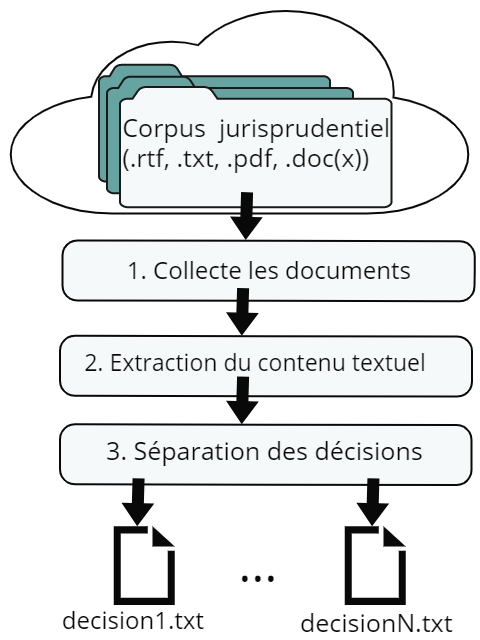
\includegraphics [width=0.45\textwidth]{structuration-preprocess.png}
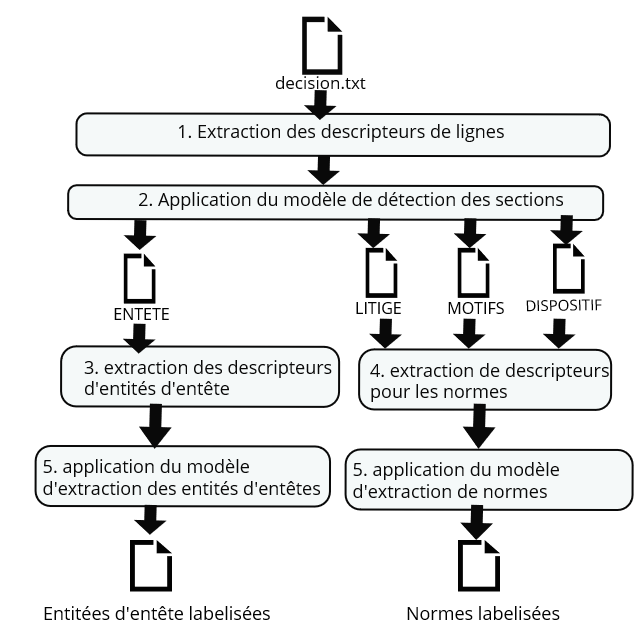
\includegraphics [width=0.45\textwidth]{structuration-pipeline-application.png}

{\scriptsize Après la collecte et le prétraitement des documents, l'étiqueteur de ligne est d'abord appliqué pour détecter les sections, puis les étiqueteurs d'entités peuvent être appliqués simultanément dans les sections.}
\caption{Application des modèles entraînés pour l'étiquetage de sections et entités.}\label{fig:structuration:archAppli}
\end{figure}
Nous proposons de travailler uniquement avec le contenu textuel des documents. Ce contenu est extrait des documents téléchargés en éliminant les éléments inutiles, principalement des espaces vides. Ces éléments sont typiques des documents formatés (\verb|.rtf, .doc(x), .pdf|). Ils ne fournissent pas une indication standard sur le début des sections. Le choix de ne pas exploiter le formatage des documents permet d'avoir à gérer un nombre plus faible de diversités entre les textes tout en appliquant le même processus de traitement à tout document indépendamment de son format d'origine. Une simple architecture d'étiquetage de sections et d'entités juridiques a été conçue avec cette uniformisation des documents comme point d'entrée (Figure \ref{fig:structuration:archAppli}). Ainsi, les documents sont collectés puis pré-traités suivant leur format d'origine (extraction du texte et séparation des décisions apparaissant dans le même document).  Ensuite, après le sectionnement des décisions, les entités sont identifiées dans les différentes sections. Par ailleurs, comme segment atomique à étiqueter nous avons choisi les lignes pour la détection des sections, et les mots pour les entités. 

\begin{figure}[!h]
%\sidecaption
\centering
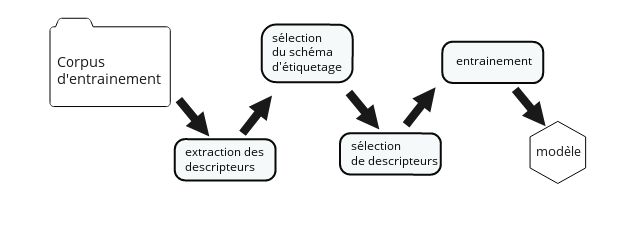
\includegraphics [width=\textwidth]{structuration-training.png}
\caption{Entrainement des modèles.}\label{fig:structuration:training}
\end{figure}


Les modèles HMM et CRF étant tous les deux supervisés, ils doivent être entraînés sur des exemples manuellement annotés pour estimer leurs paramètres. Nous proposons de sélectionner le schéma d'étiquetage et les sous-ensembles minimaux de caractéristiques manuellement définies, avant d'entraîner les modèles HMM et CRF (Figure \ref{fig:structuration:training}). 

\subsection{Définition de descripteurs candidats}

\subsubsection{Descripteurs pour la détection des sections}

Nous considérons donc la ligne comme élément à étiqueter lors du sectionnement. Nous n'avons pas travaillé au niveau des mots afin d'éviter que des mots de la même ligne ne soient classés dans des sections différentes. L'étiquetage des phrases a été aussi évité car en découpant les documents en phrases telles qu'elles sont entendues en français, on a généralement des segments qui s'étendent d'une section à une autre (absence de ponctuation). De plus, l'entête en particulier a plus l'apparence d'un formulaire.

Plusieurs critères peuvent être utilisés pour différencier les sections, à savoir: la longueur des lignes (plus longues dans le corps, plus courtes dans l'en-tête), les premiers termes de certaines lignes (typiques de chaque section) et le nombre total de lignes. Un HMM n'adapte qu'un descripteur assimilé à l'élément à étiqueter. D'autres descripteurs peuvent être la position de l'élément à étiqueter (numéro de ligne) ou le début de la ligne. Le descripteur capturant la longueur de ligne peut être absolu (nombre exact de mots dans la ligne), ou relatif (une catégorie de la longueur). Sur la base des quantiles de la distribution des longueurs de lignes sur un ensemble de décisions, nous avons défini trois catégories:
\verb|LQ1| ($longueur \leq$ 5), \verb|LQ2| (5 < $longueur \leq$ 12) et \verb|LQ2| (12 < $longueur \leq$ 14). Nous avons également catégorisé les parties de documents afin de capturer une position de ligne relative.

Lors de l'extraction des caractéristiques, le document est considéré comme divisé en $N$ parties (10 dans nos expériences). La position relative d'une ligne est donc le numéro de la partie contenant la ligne particulière. En résumé, les caractéristiques sont décrites comme suit (avec leurs étiquettes entre parenthèses):
\begin{itemize}
 \item forme de la ligne: la ligne entière, ses premiers mots (\verb|t0, t1, t2|), sa longueur absolue (\verb|absLength|) et sa longueur relative (\verb|relLength|);
 \item contexte de ligne: le numéro de ligne (\verb|absNum|) et le numéro de la partie de document contenant la ligne (\verb|relNum|), les deux premiers mots des lignes précédente (\verb|p0, p1|) et suivantes (\verb|n0, n1|), ainsi que leurs longueurs absolues et relatives
 (\verb|pLength|, \verb|pRelLength|, \verb|nLength|, \verb|nRelLength|).
\end{itemize}

\subsubsection{Descripteurs pour la détection d'entités}

La détection d'entités consiste à entraîner soit un modèle CRF, soit un modèle HMM pour étiqueter les différents segments de texte (mot, ponctuation, numéro, identifiant) suivant qu'ils appartiennent ou non à la mention d'une entité. Les deux modèles nécessitent des caractéristiques, dont certaines peuvent être définies sur la base de régularités directement observables dans les textes. Il est également possible d'obtenir des descripteurs à partir du résultat d'autres tâches d'analyse de texte.

Sur la base des observations de décision, nous avons défini la morphologie des mots pour les normes et méta-données d'entête:
\begin{itemize}
	\item forme du mot: le mot (\verb|token|), son lemme (\verb|lemma_W0|), \og commence-t-il par une lettre majuscule? \fg{} (\verb|startsWithCAP|), \og est-il entièrement en majuscule? \fg{} (\verb|isAllCAP|), \og est-ce une initiale solitaire? \fg{} comme par exemple \og B. \fg{} (\verb|isLONELYINITIAL|), \og contient-il un caractère de ponctuation? \fg{} (\verb|PUN-IN|), \og n'est-ce qu'une ponctuation? \fg{} (\verb|isALLPUN|), \og contient-il un caractère numérique? \fg{} (\verb|DIGIT-IN|),  \og ne contient-il que 
	des chiffres? \fg{} (\verb|isALLDIGIT|);
	\item contexte de mot: les mots précédents (\verb|w-2, w-1|) et suivants (\verb|w1, w2|) et leurs lemmes (\verb|lemmaW|$_i$). La lemmatisation homogénéise les variantes du même mot. Les mots adjacents sont choisis pour indiquer les termes couramment utilisés pour introduire des entités.
\end{itemize}

Plus particulièrement pour les méta-données d'entête, nous avons défini des descripteurs supplémentaires pour capter le contexte du mot: numéro de ligne (\verb|lineNum|), position de l'élément dans la ligne (\verb|numInLine|), \og le document contient-il le mot clé \textit{intervenant} ? \fg{} (\verb|intervenantInText|), le texte vient-il après le mot clé \og APPELANT \fg{} (\verb|isAfterAPPELANT|), \og INTIME \fg{} (\verb|isAfterINTIME|), \og INTERVENANT \fg{} (\verb|isAfterINTERVENANT|). Nous avons également pris en compte les dernières lignes, où le mot était précédemment rencontré dans le texte ( \verb|lastSeenAt| ), ainsi que le nombre de fois où il a été trouvé ( \verb|nbTimesPrevSeen| ), car les noms des parties sont souvent répétés à des emplacements différents. Nous avons également défini une caractéristique spéciale pour les normes: \og le mot est-il un mot clé de règles juridiques? \fg{} (\verb|isKEYWORD|). Pour ce dernier descripteur, nous avons établi une courte liste de mots-clés généralement utilisés pour citer des règles juridiques (\textit{article, code, loi, contrat, décret, convention, civil, pénal}, etc.).

Nous avons étendu ces caractéristiques avec les rôles grammaticaux (\textit{Part-of-Speech} et les modèles thématiques (\textit{topic model}).

\textbf{Rôles grammaticaux}: Certaines entités ont tendance à contenir des rôles grammaticaux particuliers. Par exemple, les noms d'individus sont composés de noms propres (Chang et Sung, 2005). Nous avons extrait le rôle grammatical du mot courant (\verb|POS|) ainsi que celui de ses voisins (\texttt{POSW-2, POSW-1, POSW1, POSW2}).

\textbf{Modèles thématiques}: comme \citet{polifroni2011usingLDA} et \citet{nallapati2010blinddomaintransferner}, nous utilisons des associations mot-thème pour décrire les mots. Il s'agit de modéliser un ensemble de $N$ thèmes et d'utiliser leurs identifiants comme descripteurs. Il serait peut-être intéressant d'utiliser la probabilité déduite du modèle thématique, mais l'inférence sous-jacente au modèle LDA \citep{blei2003lda} n'est pas déterministe (la distribution de probabilité change pour le même mot entre différentes inférences).
Néanmoins, l'ordre des sujets ne changeant pas de manière significative, nous avons utilisé l'identifiant du thème le plus pertinent pour le mot (\verb|topic0|) ainsi que ceux de ses voisins (\verb|w-2topic0|, \verb|w-1topic0|, \verb|w1topic0|, \verb|w2topic0|).

\subsection{Sélection des descripteurs}
\subsubsection{Sélection  pour le modèle CRF}
 Nous avons étudié deux approches enveloppantes qui semblent toujours converger et qui ne nécessitent pas de définir manuellement la taille du sous-ensemble cible. %Il s'agit de la recherche bidirectionnelle et de la  sélection séquentielle à flottement avant. 

\begin{algorithm}[H] \small
	\KwData{Données annotées, $X$ liste de tous les descripteurs candidats}
	\KwResult{Sous-ensemble optimal de descripteurs}
	Démarrer la SFS avec $Y_{F_0}= \emptyset $\; 
	Démarrer la SBS avec $Y_{B_0}=X$\; $k=0$\;
	\While{$Y_{F_k} \neq Y_{B_k}$}{
		$x^+=\argmax_{\substack{x \in Y_{B_k} \setminus Y_{F_k}}} F1(Y_{F_k} + x)$; 
		$Y_{F_{k+1}} = Y_{F_k} + x^+$ //SFS\;
		$x^-=\argmax_{\substack{x \in Y_{B_k} \setminus Y_{F_{k+1}}}} F1(Y_{F_k} - x)$;
		$Y_{B_{k+1}} = Y_{B_k} - x^-$ //SBS\; 
		$k = k+1$;
	}
	\Return $Y_{F_k}$\;
	\caption{Recherche bidirectionnelle BDS} \label{algo:structuration:bds}
\end{algorithm}
La première méthode, qui est la recherche bidirectionnelle (BDS) de \citet{liu2012featureSelection}, combine la sélection séquentielle en avant (SFS) et la sélection séquentielle en arrière (SBS) en parallèle (Algorithme \ref{algo:structuration:bds}). 
La SFS recherche un sous-ensemble optimal, en commençant par un ensemble vide et en ajoutant le descripteur qui améliore le mieux l'efficacité du sous-ensemble sélectionné. Le critère d'efficacité dans notre cas est défini par la F1-mesure (Eq. \ref{eq:structuration:f1mesure}). Contrairement à la SFS, la SBS commence par l'ensemble des candidats et supprime successivement les plus mauvais descripteurs. Une caractéristique ne peut être ajoutée dans $Y_{F_{k+1}}$ que si elle est présente dans $Y_{B_{k}}$.



\begin{algorithm}[H] %\small
	\KwData{Données annotées, $X$ liste de tous les descripteurs candidats}
	\KwResult{Sous-ensemble optimal de descripteurs}
	$Y_0= \emptyset $\; 
	$k=0$\;
	\Repeat{$X = \emptyset$ ou $X = Y_{k}$}{
		$x^+=\argmax_{x \notin Y_k} F1(Y_k + x)$; \label{p4_forward_sffs}
		$Y_k = Y_k + x^+$\; 
		$x^-=\argmax_{x \in Y_k} F1(Y_k - x)$\; \label{p4_back_sffs}
		\eIf{F1($Y_k - x^-$) > F1($Y_k$)}{
			$Y_{k+1} = Y_k - x^-$\; 
			$X = X - x^-$\;
			$k = k+1$\;
			Rentrer à \ref{p4_back_sffs}\;
		}{
			Rentrer à  \ref{p4_forward_sffs}\;
		}
	}
	\Return $Y_k$\;
	\caption{Sélection séquentielle avant à flottement}\label{algo:structuration:sffs}
\end{algorithm}

La seconde méthode, qui est l'algorithme de sélection séquentielle avant à flottement SFFS  de \citet{pudil1994floatingFeatSelection}, étend la SFS en surmontant son incapacité à réévaluer l'utilité d'un descripteur après son rejet. En effet, le SFFS effectue des tests en arrière à chaque itération (Algorithme \ref{algo:structuration:sffs}).

\subsubsection{Sélection pour le modèle HMM} Pour sélectionner les meilleurs descripteurs pour les modèles HMM, nous avons testé individuellement les différents candidats. La caractéristique donnant le meilleur résultat sur l'ensemble de données annotées est sélectionnée.

\section{Expérimentations et discussions}

L'objectif de cette section est de discuter des différents aspects liés à la performance des modèles CRF et HMM. Il est question de discuter l'effet des descripteurs candidats définis, de comparer des algorithmes de sélection de caractéristiques et des schémas d'étiquetage. Nous discutons par la suite l'origine des erreurs (confusion, nombre d'exemples d'entraînement), et comparons les descripteurs définis manuellement par rapport à l'utilisation de réseaux de neurones.

\label{sec:structuration:experimentations}
\subsection{Conditions d'expérimentations}
\subsubsection{Annotation des données de référence}
Pour évaluer les méthodes de TAL, \citet{xiao2010corpuscreation} suggère de choisir un jeu d'exemples suffisant en assurant au mieux l'équilibre dans la variété des données et la représentativité du langage. Nous avons essayé de suivre cette recommandation  en sélectionnant aléatoirement des décisions à annoter. Au total, 503 documents ont été rassemblés et annotés manuellement à l'aide de la plateforme GATE Developer\footnote{https://gate.ac.uk/family/developer.html}. Cet outil permet de marquer les passages à annoter en les surlignant à l'aide du pointeur de la souris; ce qui allège  l'annotation manuelle. Des balises XML sont rajoutées autour des passages sélectionnés, en arrière plan dans le document.

Chaque document annoté comprend en moyenne 262,257 lignes et 3955,215 mots. Les deux dernières colonnes du Tableau \ref{tab:structuration:relevantinfo} présentent la distribution des entités labellisées dans le jeu de données. En se basant sur un sous-ensemble de 13 documents labellisés par 2 annotateurs différents, nous avons calculé des taux d'accord inter-annotateur en utilisant la statistique Kappa de Cohen. Ces mesures d'accord inter-annotateur ont été calculées au niveau des caractères parce que certains mots peuvent être coupés par des annotations incorrectes (par ex. \textit{<juridiction> cour d'appe </juridiction> \underline{l}} contre \textit{<juridiction> cour d'appe\underline{l} </juridiction>}), ou bien les annotateurs pourraient ne pas être d'accord si une apostrophe doit être inclue ou pas dans l'annotation (par ex. \textit{ \underline{l'}<norme>article 700} contre \textit{ <norme >\underline{l'}article 700}). Les taux de Kappa de 0,705 et 0,974 ont été obtenus pour l'annotation des entités et des sections respectivement. D'après la catégorisation de \citet{viera2005kappa}, le niveau d'accord observé est \textit{substantiel} pour les entités (0,61 -- 0,80) et \textit{presque parfait} pour les sections (0,81 -- 0,99).

\subsubsection{Mesures d'évaluation}
Nous avons utilisé la précision, le rappel et la F1-mesure comme mesures d'évaluation car elles sont généralement utilisées comme références en extraction d'information. % Nous présentons aussi des performances au niveau micro c'est-à-dire en général sans distinction des classes. 
La F1-mesure se calcule à l'aide de la formule suivante:  
%\begin{equation}\label{eq:structuration:f1mesure}
\[F1 = 2 \times \frac{Precision \times Rappel} {Precision + Rappel}.\]
%\end{equation}
%La précision et le rappel quant à eux se calculent suivant les formules
% \begin{equation}\label{NER-precision}
% Precision = \frac{TP}{}
% \end{equation}

L'évaluation peut être faite au niveau des segments atomiques ou  des entités selon que l'on soit plus intéressé respectivement par l'étiquetage  du maximum de segments atomiques ou par la labellisation complète d'un maximum d'entités.

\noindent \underline{\textbf{Evaluation au niveau atomique (\textit{token-level)}}}: Cette évaluation mesure la capacité d'un modèle à labelliser les segments atomiques des entités. Les valeurs de précision et rappel sont calculées sur les données de test pour chaque label $l$ comme suit:

\[Precision_l = \frac{\text{nombre de segments correctement labelisés par le modèle avec } l} {\text{nombre de segments labelisés par le modèle avec } l}\]
\[Rappel_l = \frac{\text{nombre de segments correctement labelisés par le modèle avec } l} {\text{nombre de segments manuellement labelisés avec } l}\]

\vspace{0.3cm}

\noindent \underline{\textbf{Evaluation au niveau entité (\textit{entity-level})}}: Cette évaluation mesure le taux d'entités parfaitement identifiées c'est-à-dire seulement celles dont les segments atomiques ont été tous correctement labellisés. Les valeurs de précision et rappel sont calculés sur les données de test pour chaque classe d'entité $e$ comme suit :
\[Precision_e = \frac{\text{nombre d'entités de type } e \text{ parfaitement détectées par le modèle}} {\text{nombre d'entités détectées et classifiées } e\text{ par le modèle}}\]
\[Rappel_e = \frac{\text{nombre d'entités de type } e \text{ parfaitement détectées par le modèle}} {\text{nombre d'entitées manuellement classifiées } e}\]

\vspace{0.3cm}

\noindent \underline{\textbf{Evaluation globale (\textit{overall-level})}}: L'évaluation globale donne les performances générales d'un modèle sans distinction des classes ou labels. Elle est réalisée aux deux niveaux décrits précédemment mais indépendamment du label d'élément ou du type d'entité. La précision et le rappel sont calculées au niveau des entités comme suit:
\[Precision = \frac{\text{nombre d'entités correctement labellisées par le modèle}} {\text{nombre d'entitées labellisées par le modèle}}\]
\[Rappel = \frac{\text{nombre d'entités correctement labellisées par le modèle}} {\text{nombre d'entitées  manuellement labellisées}}.\]
Ces métriques sont calculées de la même façon au niveau atomique.

\subsubsection{Outils logiciels}
Nous avons utilisé les modèles HMM et CRF tels qu'implémentés dans la librairie Mallet \citep{McCallum2012Mallet}. Les modèles étudiés ont été entraînés par la méthode d'espérance maximale pour ceux basés sur le HMM, et par la méthode L-BFGS pour ceux basés sur le CRF. Le découpage des textes en mots (\textit{tokenisation}), la lemmatisation, et l'annotation des rôles grammaticaux (\textit{Part-of-Speech tagging}) ont été effectués à l'aide de la fonctionnalité d'annotation de textes français de TreeTagger \footnote{\url{http://www.cis.uni-muenchen.de/~schmid/tools/TreeTagger}}  \citep{schmid1994treetagger}. L'implémentation dans Mallet du LDA \citep{blei2003lda} a permis d'inférer 100 thèmes à partir d'un corpus lemmatisé d'environ 6k documents. Le tableau \ref{p4_topics} 
présente des mots représentatifs trouvés dans les premiers thèmes inférés. L'extraction des autres descripteurs a été implémentée pour cette expérimentation. 


\begin{table}[!h]
\scriptsize
\begin{center}
\begin{tabular}{c|l}
Id thème & Mots représentatifs  \\ \hline
0	& 	préjudice  dommage  somme  subir  réparation  titre  faute  payer  intérêt  responsabilité  \\ \hline
1	& société  salarié  groupe  mirabeau  pouvoir  demande  article  licenciement  cour  titre    \\ \hline
2	& harcèlement  travail  salarié  moral  employeur  fait  attestation  faire  santé  agissements  \\ \hline
3	& vente  acte  prix  vendeur  acquéreur  notaire  condition  clause  vendre  immeuble  \\ \hline
4	& 		travail  poste  reclassement  employeur  médecin  licenciement  salarié  inaptitude  visite  \\ \hline
5	& 	monsieur  nîmes  avocat  appel  barreau  arrêt  madame  disposition  prononcer  président  \\ \hline
6	& 	mademoiselle  madame  non  mesure  décision  tutelle  surendettement  comparant   \\ \hline
7	& transport  marchandise  jeune  sed  éducateur  bateau  navire  transporteur  responsabilité  \\ \hline
8	&congé  salarié  conversion  emploi  plan  convention  employeur  sauvegarde  reclassement  \\ \hline
9	&marque  site  contrefaçon  sous  droit  auteur  joseph  produit  propriété  photographie  \\ \hline
10	&pierre  patrick  bordeaux  bruno  catherine  civil  article  corinne  cour  avocat\\ \hline
\end{tabular}
\end{center}
\caption{Mots représentatifs des 10 premiers thèmes sur les 100 inférés}\label{p4_topics}
\end{table}

Les valeurs de précision, rappel, et F1-mesure ont été calculées à l'aide du script d'évaluation de la campagne CoNLL-2002 \footnote{\url{http://www.cnts.ua.ac.be/conll2002/ner/bin/conlleval.txt}}. Elles sont indiquées en pourcentage dans les tableaux de résultats d'évaluation des sections suivantes.

\subsection{Sélection du schéma d'étiquetage}
Dans le but d'évaluer comment la représentation de segment affecte les performances, nous avons implémenté quatre représentations (IO, IEO2, BIO2, BIEO).  Nous avons réalisé un simple découpage des données en deux ensembles: $25 \%$ pour l'entraînement et $75 \%$ pour les tests. Les performances reportées dans le Tableau \ref{fig:structuration:select-segm-repr} sont les performances globales sur la base de test. Seul l'élément (mot/ligne) est utilisé comme descripteur. La durée d'entraînement est très longue, particulièrement pour la détection d'entités dans l'entête avec le CRF. Il semble évident que cette durée croisse proportionnellement avec le nombre de labels candidats de la section et la complexité du schéma d'étiquetage. En effet, BIEO exige beaucoup plus de temps, et IO exige le temps d'entraînement le plus bas, et le schéma IOE semble être plus rapide que BIO même s'ils ont le même nombre de labels. Nous remarquons aussi que les représentations complexes n'améliorent pas significativement les résultats par rapport au simple IO qui demande pourtant beaucoup moins de temps.

\begin{table}[h]
\scriptsize
\begin{center}
\begin{tabular}{p{0.9cm}|c|cccccccc}
\hline \noalign{\smallskip}
Tâche & Modèle & \multicolumn{3}{c}{Niveau atomique$^a$} & \multicolumn{3}{c}{Niveau entité$^a$} & \multirow{2}{*}{Durée$^b$} & Schéma \\
 & & Précision & Rappel & F1 &  Précision & Recall & F1 &  & \\ \hline %\noalign{\smallskip}\svhline\noalign{\smallskip}
\multirow{8}{*}{Sections}  & \multirow{4}{*}{CRF} & 91.75 & 91.75 & 91.75 & 64.49 & 56.55 & 60.26 &  4.685  & IO \\
&  & 88.95 & 88.95 & 88.95 & 48.12 & 38.26 & 42.63  & 11.877 & IEO2 \\
&  & 87.09 & 87.09 & 87.09 & 46.79 & 37.20 & 41.45 & 12.256 & BIO2 \\
 &  & 86.00 & 86.00 & 86.00 & 58.98 & 41.86 & 48.97  & 35.981 & BIEO \\ \cline{2-10}
& \multirow{4}{*}{HMM} & 32.64 & 32.64 & 32.64 & 22.16 & 18.91 & 20.41 & 6.564 & IO \\
&  & 32.92 & 32.92 & 32.92 & 17.73 & 16.09 & 16.87  &   7.827  & IEO2 \\
 &  & 32.39 & 32.39 & 32.39 & 31.93 & 26.65 & 29.05 & 8.391 & BIO2 \\
  &  & 33.06 & 33.06 & 33.06 & 32.47 & 27.53 & 29.80 & 8.7 & BIEO \\ \hline %
\multirow{8}{=}{Entités d'entête}  & \multirow{4}{*}{CRF} & 86.86 & 78.96 & 82.73 & 80.84 & 65.17 & 72.17  & 70.525 & IO \\
 &  & 87.77 & 79.65 & 83.51 & 82.46 & 65.19 & 72.82  & 228.751 & IEO2 \\
 &  & 87.41 & 78.14 & 82.51 & 81.66 & 66.80 & 73.49 & 230.865 & BIO2 \\
 &  & 87.72 & 79.55 & 83.44 & 84.38 & 68.35 & 75.53 &  475.249 & BIEO \\ \cline{2-10}
  & \multirow{4}{*}{HMM} & 79.12 & 67.75 & 73.00 & 61.48 & 35.05 & 44.64 & 6.345 & IO \\
  &  & 78.82 & 68.69 & 73.40 & 66.63 & 40.16 & 50.11& 8.298 & IEO2 \\ 
  &  & 80.68 & 67.48 & 73.49 & 70.37 & 45.32 & 55.14 & 7.908 & BIO2 \\
 &  & 80.05 & 69.01 & 74.12 & 74.73 & 50.77 & 60.46 & 9.973 & BIEO \\ \hline
\multirow{8}{*}{Normes}  & \multirow{4}{*}{CRF} & 95.60 & 92.96 & 94.26 & 88.06 & 83.50 & 85.72 & 28 & IO \\%
&  & 95.40 & 93.18 & 94.27 & 88.75 & 85.65 & 87.17 & 32.136 & IEO2 \\
 &  & 95.20 & 93.30 & 94.24 & 85.65 & 83.13 & 84.37 & 50.769 & BIO2 \\
  &  & 95.46 & 91.57 & 93.47 & 88.83 & 84.71 & 86.72 & 50.566 & BIEO \\ \cline{2-10}
  & \multirow{4}{*}{HMM} & 89.83 & 88.78 & 89.30 & 73.74 & 75.02 & 74.37 &  41.389 & IO \\%  
   &  & 88.20 & 89.23 & 88.71 & 78.01 & 81.27 & 79.61 & 44.086 & IEO2 \\
  &  & 89.25 & 87.83 & 88.53 & 73.89 & 76.63 & 75.24 & 46.634 & BIO2 \\
  &  & 87.39 & 88.10 & 87.74 & 77.76 & 82.35 & 79.99 & 45.52& BIEO \\ 
\noalign{\smallskip}\hline\noalign{\smallskip}
\end{tabular}
\caption{Comparaison des schémas d'étiquetage.}\label{fig:structuration:select-segm-repr}
\end{center}

$^a$ Résultats sur une simple division du jeu de données en $25\%$ pour l'entraînement et  $75\%$ pour les tests (entraînement limité à 100 itérations au max)

$^b$ Durée d'entraînement en secondes avant l'arrêt de l'entraînement
\end{table}


\subsection{Sélection des descripteurs}
Pour comparer les méthodes BDS et SFFS, nous exploitons le schéma IO. Durant nos expérimentations, la méthode SFFS a exécuté 185 entraînements pour le modèle CRF d'identification des sections. La méthode BDS quant à elle a duré plus de 15h pour 600 itérations d'entraînement-test. Malgré la sauvegarde des scores F1 pour éviter d'exécuter plusieurs fois l'entraînement pour les mêmes sous-ensembles de descripteurs, le processus de sélection est resté toujours très long pour les deux algorithmes. Nous avons testé individuellement chacun des descripteurs candidats pour les modèles HMM. Les résultats sont reportés dans le Tableau \ref{fig:structuration:select-feats}.

\begin{table}[!htb]
\scriptsize
\begin{center}
\begin{tabular}{p{1cm}|c|ccc|ccc|c}
\hline\noalign{\smallskip}
Tâche & Modèle & \multicolumn{3}{c}{niveau atomique$^a$} & \multicolumn{3}{c}{niveau entité$^a$}& Sous-ensemble \\
 & & Précision & Rappel & F1 &  Précision & Rappel & F1 & sélectionné\\
\noalign{\smallskip}\hline\noalign{\smallskip}
\multirow{7}{*}{Sections} 		& \multirow{4}{*}{CRF} & 99.31 & 99.31 & 99.31 & 90.28 & 90.68 & 90.48 & BDS$^{b1}$  \\
  				&  & 99.55 & 99.55 & {99.55} & 85.69 & 85.84 & 85.76 & {SFFS}$^{b2}$ \\
                &  & 99.36 & 99.36 & 99.36 & 88.16 & 88.39 & 88.27 & TOUS$^{b0}$ \\
                &  & 91.75 & 91.75 & 91.75 & 64.49 & 56.55 & 60.26 & token \\  \cline{2-9}
                 & \multirow{3}{*}{HMM} & 90.99 & 90.99 & {90.99}  & 4.18 & 3.63 & 3.89 & {absLength} \\ 
 & & 86.97 & 86.97 & 86.97 & 4.08 & 3.30 & 3.65 & relLength \\   
  &  & 37.59 & 37.59 & 37.59  & 18.81 & 18.81 & 18.81 & token \\ \hline
\multirow{7}{=}{Entités d'entête}	& \multirow{4}{*}{CRF} & 94.00 & 91.42 & 92.69 & 92.26 & 88.76 & 90.47 & BDS$^{c1}$  \\
				&  & 94.10 & 91.93 & {93.00} & 92.64 & 88.96 & 90.76 & {SFFS}$^{c2}$  \\ 
                &  & 94.20 & 91.86 & 93.02 & 93.05 & 89.59 & 91.28 & TOUS$^{c0}$ \\
                &  & 86.86 & 78.96 & 82.73 & 80.84 & 65.17 & 72.17 & token \\ \cline{2-9}
                  &  \multirow{3}{*}{HMM}  & 76.90 & 80.41 & {78.61} & 62.66 & 52.16 & 56.93 &  {token} \\ 
  &    & 66.48 & 69.67 & 68.04 & 39.34 & 28.36 & 32.96 &  lemma\_W0 \\ 
  &    & 39.63 & 37.50 & 38.54 & 15.49 & 5.35 & 7.95 &  POS \\ \hline
\multirow{6}{*}{Normes} 			& \multirow{4}{*}{CRF} & 95.91 & 96.72 & 96.31 & 91.14 & 90.45 & 90.80 & {BDS}$^{d1}$ \\ 
				&  & 95.68 & 95.45 & 95.57 & 90.34 & 88.27 & 89.29 & SFFS$^{d2}$ \\ 
                &  & 95.07 & 96.69 & 95.87 & 90.87 & 90.64 & 90.76 & TOUS$^{d0}$ \\
                &  & 95.60 & 92.96 & 94.26 & 88.06 & 83.50 & 85.72 & token \\ \cline{2-9}
                 &  \multirow{2}{*}{HMM} & 89.21 & 94.25 & 91.66 & 72.67 & 77.28 & 74.90 &  \textbf{token} \\ 
  &   & 90.31 & 92.81 & 91.54 & 69.24 & 69.46 & 69.35 &  lemma\_W0 \\ 
%  \noalign{\smallskip}\svhline\noalign{\smallskip}
%  & & token-level & entity-level & \\ \hline
\noalign{\smallskip}\hline\noalign{\smallskip}
\end{tabular}

\end{center}

$^a$ Résultats sur un simple découpage des données de $25\%$ pour l'entraînement,  $75\%$ pour le test avec 100 itérations d'entraînement au maximum  pour le CRF, et $80\%$ pour l'entraînement et $20\%$ pour le test avec 50 itérations au maximum pour l'entraînement du HMM

$^{b0}$ \textbf{Tous les candidats définis pour les sections (16 descripteurs) }: $\lbrace$ relNum, relLength, pRelLength, absLength, t0, t1, t2, absNum, pLength, nRelLength, n0, nLength, p0, p1, n1, token $\rbrace$ 

$^{b1}$ \textbf{Selection par BDS pour les sections (07 descripteurs)} : $\lbrace$p0, n0, relNum, absLength, t0, t1, t2$\rbrace$ 

$^{b2}$ \textbf{Selection par SFFS pour les sections (06 descripteurs)} : $\lbrace$ n0, nRelLength, relNum, t0, t1, t2 $\rbrace$ 

$^{c0}$ \textbf{Tous les candidats définis pour les méta-données d'entête (34 descripteurs)} : $\lbrace$ isLONELYINITIAL, isALLCAP, isALLDIGIT, DIGIT-IN, intervenantInText, lineNum, lastSeenAt, nbTimesPrevSeen, isAfterAPPELANT, isAfterINTIME, isAfterINTERVENANT, startsWithCAP, PUN-IN, isALLPUN, POSW2, w2topic0, numInLine, POSW-1, lemmaW2, lemmaW-2, POSW-2, w-2topic0, POSW1, w1topic0, token, POS, lemma\_W0, topic0, w2, w-1topic0, lemmaW-1, w-1, w1, lemmaW1 $\rbrace$ 

 $^{c1}$ \textbf{Selection par BDS pour les méta-données d'entête (17 descripteurs) }:  $\lbrace$ POSW1, isAfterAPPELANT, numInLine, w-2topic0, POSW2, isAfterINTERVENANT, isAfterINTIME, POSW-2, isLONELYINITIAL, token, lemma\_W0, lemmaW-2, isALLPUN, w-1, w1, w2, isALLCAP $\rbrace$ 

$^{c2}$ \textbf{Selection par SFFS pour les  entités d'entête (10 descripteurs)}: $\lbrace$ numInLine, w-2topic0, lemmaW-2, isAfterINTERVENANT, isAfterINTIME, w-1, w1, w2, isALLCAP, token $\rbrace$ 

$^{d0}$ \textbf{Tous les candidats définis pour les normes (28 descripteurs)} : $\lbrace$ isALLPUN, isALLDIGIT, DIGIT-IN, isKEYWORD, POSW2, w2topic0, PUN-IN, POSW-1, isLONELYINITIAL, startsWithCAP, isALLCAP, lemmaW-2, POSW-2, w-2topic0, POS, topic0, POSW1, w1topic0, w2, lemmaW2, token, lemma\_W0, w-2, w-1topic0, w-1, lemmaW-1, w1, lemmaW1 $\rbrace$ 

$^{d1}$ \textbf{Selection par BDS pour les normes (14 descripteurs)} : $\lbrace$ POSW1, w-2topic0, isKEYWORD, lemmaW2, DIGIT-IN, token, lemmaW1, lemmaW-2, POS, isALLPUN, w-1, w2, PUN-IN, w-2 $\rbrace$ 

$^{d2}$ \textbf{Selection par SFFS pour les normes (04 descripteurs)}: $\lbrace$POSW1, lemmaW-2, w-1, DIGIT-IN$\rbrace$ 

\caption{Performances des sous-ensembles sélectionnés de descripteurs.}\label{fig:structuration:select-feats}
\end{table}

Le résultat le plus remarquable est la forte réduction du nombre de descripteurs par les algorithmes. En général, la moitié est éliminée par la sélection BDS, tandis que la méthode SFFS élimine beaucoup plus de candidats (par exemple en ne sélectionnant que 4 descripteurs parmi les 14 candidats définis pour l'annotation des normes).

Par ailleurs, les algorithmes de sélection forment des combinaisons inattendues. Par exemple, dans le cas de la détection de section, la ligne suivante semble être beaucoup plus indicatrice que la première. Il est aussi intéressant de noter que les descripteurs basés sur notre observation apparaissent dans les sous-ensembles sélectionnés (par ex. \verb|isAfterIntervenant|, \verb|isKEYWORD|). Remarquons aussi que la longueur absolue des lignes (\verb|absLength|)  joue un rôle important dans l'identification des sections vu qu'il a été sélectionné à la fois pour le CRF et le HMM (sélection BDS). Avec ces sous-ensembles sélectionnés, les modèles sont plus performants que lorsqu'ils exploitent seulement le segment ou l'ensemble tout entier des candidats.  Cette amélioration des résultats n'est pas très importante au regard de la longue durée d'exécution des algorithmes. Ainsi, un algorithme plus rapide et plus efficace devrait être utilisé.


\subsection{Evaluation détaillée pour chaque classe}
Nous discutons ici la capacité des modèles à identifier individuellement chaque type d'entité et de section. Les expérimentations ont été réalisées avec tous les descripteurs pour les modèles CRF. Seuls \verb|absLength| et \verb|token| ont été utilisés comme descripteurs dans les modèles HMM pour l'identification des sections et des entités respectivement. Le schéma d'étiquetage est IO. Le nombre d'itérations maximal a été fixé à 500 pour assurer la convergence lors de l'entraînement même si les modèles HMM ne convergeaient jamais après 500 itérations. Les Tableaux \ref{tab:structuration:perf-detail-token} et \ref{tab:structuration:perf-detail-entity} présentent les résultats d'une validation croisée à 5 itérations, respectivement aux niveaux atomique et entité. D'un point de vue général (évaluation globale), les modèles HMM se comportent assez bien au niveau élément avec un seul descripteur, particulièrement pour l'identification des sections et des normes. Le modèle HMM est capable de labelliser les normes car plusieurs d'entre elles sont répétées entre les décisions. De plus, la citation des normes est quasi standard (\verb|article [IDENTIFIANT] [TEXTE D'ORIGINE]|). Le modèle HMM n'est cependant pas aussi efficace pour détecter entièrement les mots des entités d'où le faible score enregistré au niveau entité. Quant aux modèles CRF, leurs résultats sont très bons sur toutes les tâches et à tous les niveaux d'évaluation malgré quelques limites observées sur l'identification des parties.
\begin{table}[!h]
	\centering
	\scriptsize
	\begin{tabular}{|l|l|l|l|l|l|l|}
		\hline
	\multirow{2}{*}{}	& \multicolumn{3}{c}{\textbf{HMM}}  &      \multicolumn{3}{|c|}{\textbf{CRF}}          \\ \cline{2-7}
		& \textit{Precision} & \textit{Rappel} & \textit{F1} & \textit{Precision} & \textit{Rappel} & \textit{F1} \\ \hline
		\textbf{I-corps}       & 92.46              & 95.25           & 93.83       & 99.57              & 99.69           & 99.63       \\ 
		\textbf{I-dispositif}  & 53.44              & 48.46           & 50.83       & 98.63              & 97.59           & 98.11       \\ 
		\textbf{I-entete}      & 97.91              & 91.93           & 94.83       & 99.51              & 99.55           & 99.53       \\ \hline
		\textbf{Evaluation globale}       & 90.63              & 90.63           & 90.63       & 99.48              & 99.48           & 99.48       \\ \hline
		\noalign{\smallskip}\hline\noalign{\smallskip}
		\textbf{I-appelant}    & 34.46              & 16.87           & 22.65       & 84.34              & 76.27           & 80.1        \\ 
		\textbf{I-avocat}      & 85.17              & 98.75           & 91.46       & 98.02              & 98.15           & 98.09       \\ 
		\textbf{I-date}        & 75.67              & 72.45           & 74.02       & 98                 & 96.6            & 97.3        \\ 
		\textbf{I-fonction}    & 88.81              & 64.46           & 74.7        & 95.23              & 95.13           & 95.18       \\ 
		\textbf{I-formation}   & 79.38              & 94.38           & 86.23       & 98.8               & 99.45           & 99.12       \\ 
		\textbf{I-intervenant} & 82.07              & 38.04           & 51.98       & 83.38              & 68.26           & 75.07       \\ 
		\textbf{I-intime}      & 50.4               & 68.09           & 57.93       & 82.54              & 83.33           & 82.93       \\ 
		\textbf{I-juge}        & 73.4               & 88.73           & 80.34       & 97.55              & 97.23           & 97.39       \\ 
		\textbf{I-juridiction} & 85.15              & 98.37           & 91.28       & 98.91              & 99.69           & 99.3        \\ 
		\textbf{I-rg}          & 68.53              & 22.14           & 33.47       & 97.81              & 97.44           & 97.62       \\ 
		\textbf{I-ville}       & 91.5               & 82.41           & 86.72       & 98.94              & 99.15           & 99.04       \\ \hline
		\textbf{Evaluation globale}       & 76.21              & 82.26           & 79.12       & 95.13              & 94.51           & 94.82       \\ \hline
		\noalign{\smallskip}\hline\noalign{\smallskip}
		\textbf{I-norme}       & 88.23              & 93.7            & 90.89       & 97.14              & 96.09           & 96.62       \\ \hline
	\end{tabular}
	\caption{Précision, Rappel, F1-mesures pour chaque type d'entité et section au niveau atomique.}\label{tab:structuration:perf-detail-token}
\end{table}


\begin{table}[!h]
	\scriptsize
	\centering
	\begin{tabular}{|l|l|l|l|l|l|l|}
		\hline
	\multirow{2}{*}{}	& \multicolumn{3}{c}{\textbf{HMM}}  &      \multicolumn{3}{|c|}{\textbf{CRF}}          \\ \cline{2-7}
		& \textit{Precision} & \textit{Rappel} & \textit{F1} & \textit{Precision} & \textit{Rappel} & \textit{F1} \\ \hline
		\textbf{corps}         & 0.99               & 0.99            & 0.99        & 89.57              & 90.1            & 89.83       \\ 
		\textbf{dispositif}    & 12.05              & 7.33            & 9.11        & 98.02              & 97.82           & 97.92       \\ 
		\textbf{entete}        & 10.47              & 10.5            & 10.48       & 92.11              & 92.48           & 92.29       \\ \hline
		\textbf{Evaluation globale} & 7.22               & 6.27            & 6.71        & 93.22              & 93.47           & 93.34       \\ \hline
				\noalign{\smallskip}\hline\noalign{\smallskip}
		\textbf{appelant}      & 17.84              & 5.6             & 8.52        & 84.05              & 77.29           & 80.53       \\ 
		\textbf{avocat}        & 44.29              & 39.15           & 41.56       & 90.97              & 90.3            & 90.63       \\ 
		\textbf{date}          & 66.87              & 62.15           & 64.43       & 97.96              & 96.6            & 97.27       \\ 
		\textbf{fonction}      & 89.84              & 64.13           & 74.84       & 96.89              & 96.94           & 96.92       \\ 
		\textbf{formation}     & 61.5               & 65.86           & 63.61       & 98.4               & 98.95           & 98.68       \\ 
		\textbf{intervenant}   & 14.29              & 4               & 6.25        & 62.5               & 40              & 48.78       \\ 
		\textbf{intime}        & 30.28              & 27.47           & 28.8        & 79.31              & 78.93           & 79.12       \\ 
		\textbf{juge}          & 73.54              & 83.21           & 78.07       & 96.58              & 96.35           & 96.47       \\ 
		\textbf{juridiction}   & 81.31              & 87.66           & 84.37       & 98.86              & 99.54           & 99.2        \\ 
		\textbf{rg}            & 68.53              & 22.41           & 33.77       & 97.57              & 98.02           & 97.79       \\ 
		\textbf{ville}         & 89.52              & 84.7            & 87.05       & 98.85              & 99.15           & 99          \\ \hline
		\textbf{Evaluation globale} & 64.59              & 54.56           & 59.15       & 93.77              & 92.93           & 93.35       \\ \hline
				\noalign{\smallskip}\hline\noalign{\smallskip}
		\textbf{norme}         & 71.94              & 78.45           & 75.05       & 92.66              & 91.38           & 92.01       \\ \hline
	\end{tabular}
	\caption{Précision, Rappel, F1-mesures pour chaque type d'entité et section au niveau entité.}\label{tab:structuration:perf-detail-entity}
\end{table}

\subsection{Discussions}
\subsubsection{Confusion de classes}
Certaines erreurs sont probablement dues à la proximité des entités de types différents. D'après la matrice de confusion des méta-données d'entête (Figure \ref{fig:structuration:matrice-confusion-entete}), les \textit{intervenants} sont parfois classifiés comme \textit{appelant, intimé} ou \textit{avocat} probablement parce qu'il s'agit d'entités mentionnées les unes à la suite des autres dans l'entête (les \textit{intervenants} sont mentionnés juste après les \textit{avocats} des \textit{intimés}). De plus, les intervenants apparaissent dans une très faible proportion de documents annotés.  Par ailleurs, une quantité considérable d'\textit{appelants} sont aussi classifiés comme \textit{intimés}. 

\begin{figure}[h!]
    \centering
    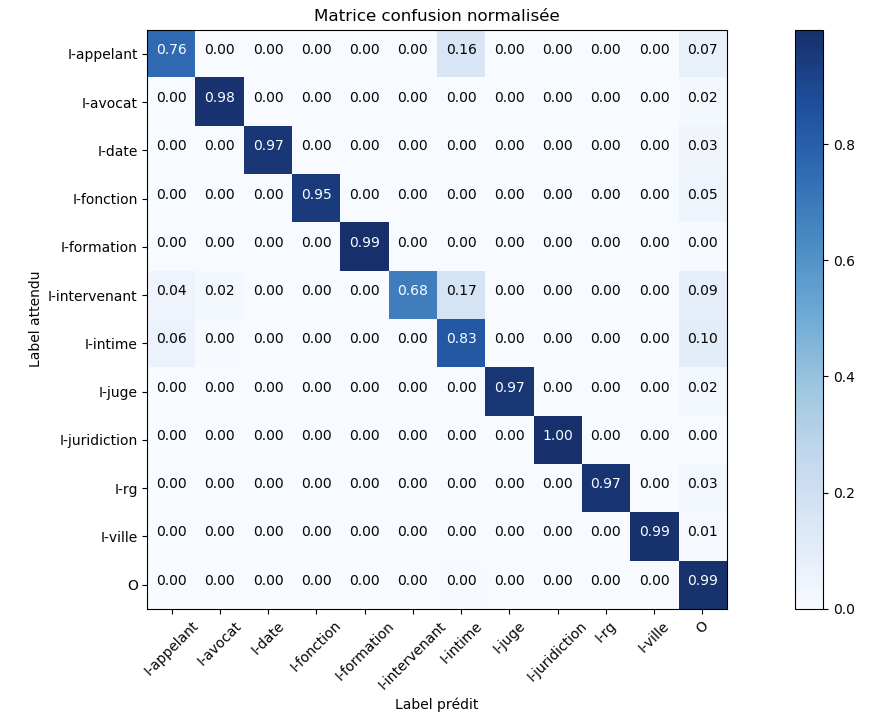
\includegraphics[width=0.8\textwidth]{confusion_matrix_entete.png}
    %\textcolor{red}{Matrices de confusion}
    \caption{Matrice de confusion entre méta-données d'entête avec le modèle CRF}
    \label{fig:structuration:matrice-confusion-entete}
\end{figure}

 La proximité crée aussi des confusions entre les sections CORPS et DISPOSITIF qui se suivent (Figure \ref{fig:structuration:matrice-confusion-section}). 

\begin{figure}[h!]
	\centering
	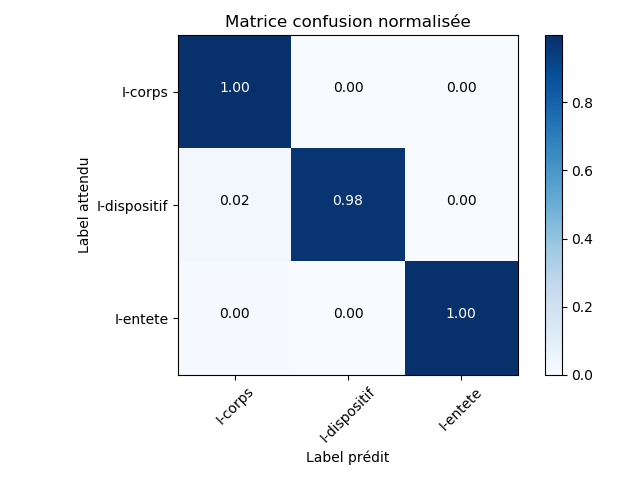
\includegraphics[width=0.6\textwidth]{confusion_matrix_section.png}
	%\textcolor{red}{Matrices de confusion}
	\caption{Matrice de confusion entre lignes des sections avec le modèle CRF}
	\label{fig:structuration:matrice-confusion-section}
\end{figure}

\subsubsection{Redondance des mentions d'entités}
Il est aussi intéressant de remarquer que certaines entités sont répétées dans le document. Par exemple, les noms des parties apparaissent précédemment à une mention qui donne plus de détails. Certaines normes sont aussi citées plusieurs fois et en alternant souvent les formes abrégées et longues (par exemple, la juridiction, la date, les normes). Bien que les mentions répétées ne soient pas identiques, de telles redondances aident à réduire le risque de manquer une entité. %certains contextes peuvent être plus favorables à la détection que d'autres
Cet aspect peut être exploité afin de combler l'imperfection des modèles.


\subsubsection{Impact de la quantité d'exemples annotés}
\begin{figure}[!h]
	\centering
	\begin{subfigure}[t]{0.95\textwidth}
		\centering
		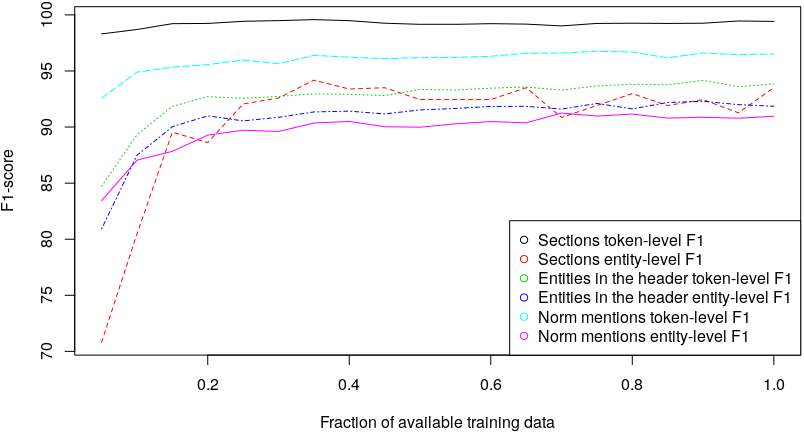
\includegraphics[width=0.85\textwidth]{lc-crf.png}
		\caption{CRF} \label{fig:structuration:learning-curves-crf}
	\end{subfigure} 
	
	\begin{subfigure}[t]{0.95\textwidth}
		\centering
		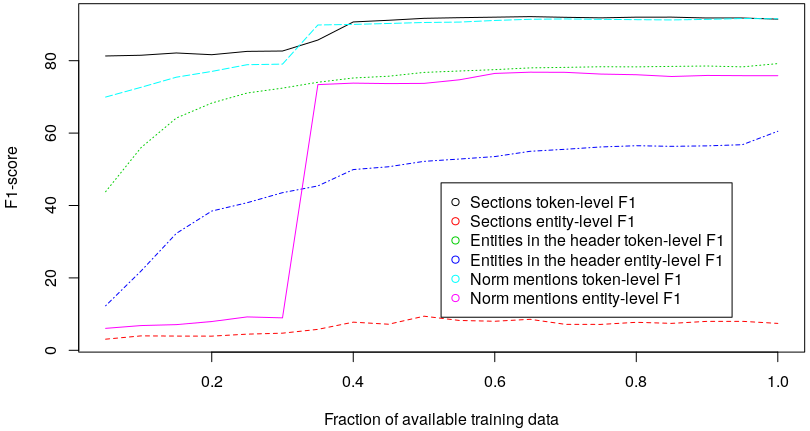
\includegraphics[width=0.85\textwidth]{lc-hmm.png}
		\caption{HMM} \label{fig:structuration:learning-curves-hmm}
	\end{subfigure}
	\caption{Courbes d'apprentissages aux niveaux élément et entité} \label{fig:structuration:learning-curves}
\end{figure}

Des expérimentations ont été menées pour évaluer la manière dont les modèles s'améliorent lorsqu'on augmente le nombre de données d'entraînement. Pour cela, nous avons évalué différentes tailles de la base d'entraînement. Les données ont été divisées en $75\%-25\%$ pour resp. l'entraînement et le test. 20 fractions de l'ensemble d'entraînement ont été utilisées  (de 5\% à 100\%). A chaque session entraînement-test, le même jeu de test a été employé pour les différentes fractions de l'ensemble d'entraînement. Les courbes d'apprentissage des modèles CRF et HMM sont représentées resp. sur les Figures \ref{fig:structuration:learning-curves-crf} et \ref{fig:structuration:learning-curves-hmm}. Il est évident que les scores F1 croissent avec le nombre de données d'entraînement pour les CRF et HMM, mais cette amélioration devient très faible au-delà de 60\% de données d'entraînement quelle que soit la tâche. Il est possible que les exemples ajoutés à partir de là partagent la même structure que celle de ceux qui ont été ajoutés auparavant. Ainsi, cette étude doit être étendue à la sélection des exemples les plus utiles. \citet{raman2003exampleSelection} ont démontré les avantages des algorithmes de sélection d'exemples combinés à celle des caractéristiques pour la classification. Les mêmes méthodes sont probablement applicables à l'étiquetage de séquences.



\subsubsection{Descripteurs manuels vs. réseau de neurones}

\begin{table}[!h]
	\scriptsize
	\centering
	\begin{tabular}{|l|l|l|l|l|l|l|}
		\hline
		&               \multicolumn{3}{c}{\textbf{CRF + descripteurs manuels}} & \multicolumn{3}{|c|}{\textbf{BiLSTM-CRF}}   \\ \cline{2-7}
		& \textit{Precision} & \textit{Rappel}                     & \textit{F1} & \textit{Precision} & \textit{Rappel}      & \textit{F1} \\ \hline
		\textbf{appelant}      & 82.49              & 69.42                               & 74.72       & 80.26              & 71.53                & 75.04       \\ 
		\textbf{avocat}        & 90.15              & 89.02                               & 89.56       & 84.93              & 87.88                & 86.36       \\ 
		\textbf{date}          & 95.34              & 91.46                               & 93.12       & 95.04              & 90.79                & 92.63       \\ 
		\textbf{fonction}      & 95.87              & 95.08                               & 95.44       & 92.69              & 93.48                & 93.03       \\ 
		\textbf{formation}     & 96.91              & 91.31                               & 93.7        & 91.05              & 89.47                & 89.84       \\ 
		\textbf{intervenant}   & 51.42              & 32.71                               & 36.8        & 31.48              & 20                   & 23.11       \\ 
		\textbf{intime}        & 76.01              & 79.15                               & 77.22       & 67.7               & 75.43                & 70.83       \\ 
		\textbf{juge}          & 95.67              & 94.07                               & 94.84       & 95.44              & 95.56                & 95.46       \\ 
		\textbf{juridiction}   & 98.55              & 98.25                               & 98.33       & 97.95              & 99.22                & 98.57       \\ 
		\textbf{rg}            & 95.46              & 95.29                               & 95.27       & 91.13              & 97.26                & 93.92       \\ 
		\textbf{ville}         & 98.33              & 93.01                               & 94.71       & 91.43              & 95.34                & 93.3        \\ 
		\textbf{norme}         & 91.08              & 90.27                               & 90.67       & 91.43              & 92.65                & 92.03       \\ \hline
		\noalign{\smallskip}\hline\noalign{\smallskip}
		\textbf{Evaluation globale} & 92.2               & 90.09                               & 91.12       & 89.21              & 90.43                & 89.81       \\ \hline
	\end{tabular}
	\caption{Comparaison entre le CRF avec des descripteurs définis manuellement et le BiLSTM-CRF au niveau entité.}\label{tab:structuration:perf-bilstmcrf}
\end{table}

L'ingénierie manuelle des caractéristiques est difficile car arbitraire. Nous avons comparé les performances de nos descripteurs avec celles des réseaux de neurones qui apprennent une représentation des segments. Pour cela nous avons choisi le BiLSTM-CRF de \citet{lample2016nnner} qui fait partie des meilleures approches récentes. La comparaison a été effectuée pour la détection des entités avec le schéma d'étiquetage BIEO et une validation croisée à 9 itérations. Le BiLSTM-CRF prend en entrée les plongements sémantiques Word2Vec des mots. Pour cela, nous avons entraîné des vecteurs de mots à partir d'un corpus jurisprudentiel de plus de 800K documents provenant de \url{www.legifrance.gouv.fr} avec l'implémentation\footnote{\url{https://code.google.com/archive/p/word2vec/}} de \citet{lemikolov2014word2vec}. Les vecteurs obtenus ont une dimension de 300. Etant donné que les décisions sont des documents particulièrement longs, leur contenu a été découpé en des morceaux de texte dont la taille n'excède pas 300 mots. Les résultats obtenus par le BiLSTM-CRF sont assez proches de ceux que nous observons avec les descripteurs manuellement définis (Tableau \ref{tab:structuration:perf-bilstmcrf}) . Etant donné que ces derniers permettent de mieux détecter certaines entités comme les \textit{intervenants}, les \textit{avocats} ou les numéro \textit{R.G.}, et vice-versa pour les \textit{normes} ou les \textit{appelants} chez le BiLSTM-CRF, une combinaison des deux types de descripteurs pourrait améliorer les résultats actuels. %On peut par exemple exploiter des modèles thématiques déduits en partitionnant (\textit{clustering}) l'ensemble des vecteurs de mots  et les utiliser comme descripteurs définis manuellement. 
 

\section{Conclusion}
\label{sec:structuration:conclusion}
L'application des modèles HMM et CRF dans le but de détecter des sections et des entités dans les décisions de justice est une tâche difficile. Ce chapitre a examiné les effets de divers aspects de la conception sur la qualité des résultats. En résumé, malgré une importante réduction du nombre de descripteurs, l'amélioration des résultats semble être insignifiante lorsque l'on sélectionne séparément la représentation du segment et le sous-ensemble de caractéristiques. Cependant, opter pour la bonne configuration en évaluant les approches de sélection combinés avec diverses représentations de segment pourrait peut-être offrir de meilleurs résultats. En raison de la longue durée de recherche du sous-ensemble optimal de descripteurs, il serait préférable d'utiliser un algorithme de sélection beaucoup plus rapide que les méthodes BDS et SFFS que nous avons expérimentées. De plus, même si les résultats s'améliorent avec la croissance de l'échantillon d'apprentissage, la mesure globale F1 semble néanmoins atteindre une limite très rapidement. Étant donné que certaines entités ne sont pas très bien détectées, il peut être avantageux d'ajouter des exemples appropriés afin de traiter ces problèmes spécifiques.

L'application des modèles pose deux difficultés majeures: l'annotation d'un nombre suffisant d'exemples et la définition de caractéristiques discriminantes. Les efforts d'annotation peuvent être réduits avec un système automatique à faible performance d'étiquetage. Il suffirait alors de vérifier manuellement ces annotations afin de corriger les erreurs commises par le système sur de nouvelles décisions à l'aide d'un outil d'aide à l'annotation. En ce qui concerne la définition des caractéristiques, dans la mesure où notre approche actuelle est réalisée manuellement par l'analyse de quelques documents, il est possible que de tels descripteurs ne s'adaptent pas parfaitement à un nouvel ensemble de données (différents pays, différentes langues, différentes juridictions). Pour éviter les énormes efforts requis pour définir les fonctionnalités manuellement, il serait préférable d'utiliser des descripteurs appris automatiquement à partir de corpus étiquetés ou non, comme des mots incorporés.

Dans les travaux futurs, il serait intéressant d'achever la tâche de reconnaissance d'entités nommées. Pour l'indexation des décisions dans une base de connaissances, il est en effet essentiel de définir des méthodes de désambiguïsation et de résolution pour les entités à occurrences multiples, en plus de la correspondance des entités extraites avec des entités de référence, comme l'ont expérimenté \citet{dozier2010legalnerr} et \citet{cardellino2017legalNERCL}. Ces travaux peuvent être poursuivis par d'autres applications telles que l'anonymisation automatique qui aiderait à publier plus rapidement l'énorme volume de décisions prononcées régulièrement.	% INCLUDE: structuration
\chapter{Extraction des données concernant les demandes et leurs résultats correspondants}
%\chapter{Extraction des demandes et résultats correspondants}
\label{chap:quanta}

\section{Introduction}
\label{sec:quanta:introduction}
Au c\oe{}ur de l'analyse des décisions de justice se trouve le concept de demande. Il s'agit d'une réclamation ou requête effectuée par une ou plusieurs parties aux juges. Une partie peut demander des dommages-intérêts en réparation d'un préjudice subi ou à l'issu d'un divorce, des indemnités auxquelles elle pense avoir droit, ou encore une étude d'expert, etc. Les demandes sont fondamentales car l'argumentation au cours d'une affaire a deux buts : faire accepter ses demandes, et faire rejeter celle de la partie adverse. L'extraction des demandes et des résultats correspondants, dans un corpus, permet ainsi de récolter des données informant de la manière dont sont jugés des types de demandes d'intérêt. Les informations qui nous intéressent sont la catégorie de la demande, le quantum (montant) demandé, le sens du résultat (par ex. la demande a-t-elle été acceptée ou rejetée?), et le quantum obtenu (décidé par les juges). Pour pouvoir extraire les demandes et les résultats, il est nécessaire de comprendre comment ils sont exprimés et co-référencés dans les décisions jurisprudentielles. Leur énoncé peut comporter des expressions plus ou moins complexes, dont souvent des références à des jugements antérieurs, des agrégations ou des restrictions (Figure \ref{fig:quanta:expr-dmd-rst}).

\begin{figure}[h]
	\scriptsize
	\centering
	\begin{subfigure}[t]{0.95\textwidth}
		\fbox{\parbox{\textwidth}{Jennifer M., Catherine M. et Sandra M. ... demandent à la Cour de :
				
				- les recevoir régulièrement appelantes incidentes du \textcolor{blue}{jugement du 23/05/2014} ;
				
				- infirmer \textcolor{blue}{le dit jugement} en \textcolor{brown}{toutes ses dispositions} ; ...
				
				Statuant à nouveau ...
				
				- \textcolor{brown}{les condamner au paiement d'une somme de  3 000,00 \euro{} pour procédure abusive et aux entiers dépens} ; }}
		\caption{Exemples d'énoncés de demandes}\label{fig:quanta:expr-dmd}
	\end{subfigure} 
	
	
	\begin{subfigure}[t]{0.95\textwidth}
		\fbox{\parbox{\textwidth}{La cour, ...  
				
				CONFIRME \textcolor{blue}{le jugement entreprise} en \textcolor{brown}{toutes ses dispositions}.
				
				Y ajoutant
				
				\textcolor{gray}{CONSTATE que Amélanie Gitane P. épouse M. est défaillante à rapporter la preuve
					d'une occupation trentenaire lui permettant d'invoquer la prescription
					acquisitive de la parcelle BH 377 située [...].}
				
				\textcolor{gray}{DEBOUTE Amélanie Gitane P. épouse M. de sa demande en dommages et intérêts.}
				
				\textcolor{gray}{CONDAMNE Amélanie Gitane P. épouse M. aux dépens d'appel.}
				
				\textcolor{gray}{DIT n'y avoir lieu à l'application de l'article 700 du Code de Procédure Civile.}
		}}
		\caption{Exemple d'énoncés de résultats}\label{fig:quanta:expr-rst}
	\end{subfigure}
	\caption{Enoncés \textcolor{gray}{simples}, ou comprenant des  \textcolor{blue}{références} et  des \textcolor{brown}{agrégations} (extraits de la décision 14/01082 de la cour d'appel de Saint-Denis (Réunion))}\label{fig:quanta:expr-dmd-rst}
\end{figure}


\subsection{Données cibles à extraire}

\subsubsection{Catégorie de demande}

Une catégorie $c$ de demande regroupe les prétentions qui sont de même nature par le fait qu'elles partagent deux aspects: l'objet demandé (par ex. dommages-intérêts, amende civile, déclaration de créance) et le fondement c'est-à-dire les règles ou normes ou principes juridiques qui fondent la demande (par ex. article 700 du code de procédure civile). Des noms particuliers sont utilisés pour identifier les catégories (Tableau \ref{tab:quanta:exemple-categorie}).

\begin{table}[!htb]
\scriptsize
\begin{tabular}{|c|p{0.35\textwidth}|p{0.15\textwidth}|p{0.3\textwidth}|}
\hline
\textbf{Label} & \textbf{Expression nominative }                                     & \textbf{Objet}                                                       & \textbf{Fondement}                                                                 \\ \hline
acpa & amende civile pour abus de procédure                         & amende civile                                               & Articles 32-1 code de procédure civile + 559 code de procédure civile  \\ \hline
concdel & dommages-intérêts pour concurrence déloyale                  & dommages-intérêts                                           & Article 1382 du code civil                                             \\ \hline
danais & dommages-intérêts pour abus de procédure                   & dommages-intérêts                                           & Articles 32-1 code de procédure civile + 1382 code de procédure civile \\ \hline
dcppc & déclaration de créance au passif de la procédure collective  & déclaration de créance & L622-24 code de commerce                                               \\ \hline
doris & dommages-intérêts pour trouble de voisinage                  & dommages-intérêts                                           & principe de responsabilité pour trouble anormal de voisinage           \\ \hline
styx & frais irrépétibles                                          & dommages-intérêts                                           & Article 700 du code de procédure civile                                 \\ \hline
\end{tabular}
\textit{Les labels ont été définis particulièrement pour cette étude, et par conséquent, ils n'existent pas dans le langage juridique.}
\caption{Exemples de catégories de demandes}\label{tab:quanta:exemple-categorie}
\end{table}

\subsubsection{Quantum demandé}

Le quantum demandé quantifie l'objet de la demande. Nous le notons $q_d$. Par exemple, dans l'exemple de la Figure \ref{fig:quanta:expr-dmd}, "3000 \euro{}" est le quantum demandé au titre des dommages-intérêts pour procédure abusive. Bien que cette étude ne porte que sur des sommes d'argent, le quantum peut être d'une autre nature comme par exemple une période dans le temps (garde d'enfant, ou emprisonnement, etc.). Toutes les catégories demandes n'ont pas de quantum (par ex. une demande de divorce) et seul le sens du résultat sera la donnée à extraire dans ce cas.

\subsubsection{Sens du résultat}

Le sens du résultat est l'interprétation de la décision des juges sur une demande. Nous le notons $s_r$. En général, le sens peut être positif si la demande a été acceptée, et négatif si elle a été rejetée. Il arrive aussi que le résultat soit reporté à un jugement futur; il s'agit dans ce cas d'un sursis à statuer. 

\subsubsection{Quantum obtenu ou résultat}

Le quantum obtenu quantifie le résultat ou la décision des juges. Nous le notons $q_r$. Il est en général inférieur ou égal au quantum demandé. Si la demande est rejetée, 
$q_r$ est évidemment nul même si cela n'est pas explicitement mentionné dans le document. Il doit être de la même nature que le quantum demandé (somme d'argent ou durée).


\subsection{Expression, défis et indicateurs d'extraction}

Les demandes sont, en général, décrites à la fin de la section d'exposé des faits, procédures, moyens et prétentions des parties (section Litige). Elles rentrent donc dans les "moyens et prétentions des parties" qui regroupent les demandes et les arguments des parties. Quant aux résultats, ils sont décrits dans la section Dispositif et dans la section Motifs (raisonnement des juges). Les demandes sont exprimées en paragraphe où chaque paragraphe correspond soit à une partie, soit à un groupe de partie partageant les mêmes demandes (par ex. des époux). Le paragraphe est parfois organisé en liste dont chaque élément exprime une ou plusieurs demandes, ou fait référence à un jugement antérieur. Les résultats ont aussi la forme de liste dans la section Dispositif. Par contre, dans les motifs de la décision, les raisonnements sont organisés en paragraphes, et ordonnés catégorie après catégorie. Le résultat est donné à la fin du groupe de paragraphes associé à la catégorie.


 Cette pseudo-structure n'est pas standard et elle impose de nombreux défis à relever. En effet, une décision jurisprudentielle porte sur plusieurs demandes de catégories différentes ou similaires. Il est important de faire correspondre un quantum demandé extrait au sens et quantum du résultat qui font référence à la même demande. La séparation des demandes et des résultats rend difficile cette mise en correspondance. Ce problème peut aussi être causé par la redondance des quanta; par exemple, les résultats exprimés dans les Motifs sont résumés dans le Dispositif. D'autre part, les références aux jugements antérieurs exigent de résoudre des références aux résultats de jugements antérieurs qui sont, généralement, rappelés dans le même document. Notons aussi que les difficultés liées aux agrégations (par ex. "\textit{infirmer ... en toutes ces dispositions}") et aux restrictions/sélections (par ex. "\textit{infirme le jugement ... sauf en ce qu'il a condamné M. A. ...}") devraient être résolues. Par ailleurs, les catégories de demandes sont nombreuses\footnote{plus de 500 selon la nomenclature des affaires civiles NAC+} mais ne sont pas toutes présentes à la fois dans les décisions. Tous ces aspects rendent difficile l'annotation manuelle des données de référence et la modélisation d'une approche d'extraction adéquate. Cependant, nous avons remarqué quelques indicateurs qui pourraient être utiles.

On pourrait au préalable annoter les candidats potentiels de quanta. Nous nous sommes intéressés aux demandes dont les quanta sont des sommes d'argent. Les mentions de somme d'argent sont généralement de la forme \og \texttt{[valeur] [monnaie]} \fg{} (par ex. \texttt{3000 \euro}, \texttt{15 503 676 francs}, \texttt{un euro}, \texttt{339.000 XPF}). Des centimes apparaissent parfois (par ex. \texttt{dix huit euros et soixante quatorze centimes}, \texttt{26'977 \euro{}  19}).  Ainsi, il est possible d'annoter les sommes d'argent à l'aide d'une expression régulière. Même s'il est difficile de reconnaître des sommes d'argent écrites en lettre, il faut remarquer que l'équivalent en chiffre est généralement mentionné tout près (par ex. \texttt{neuf mille cinq cent soixante six euros et quatre vingt sept centimes (9566,87 \euro{}  )}). 

La terminologie utilisée est aussi un bon indicateur pour reconnaître des demandes et des résultats. En effet, le vocabulaire utilisé est très souvent propre aux catégories de demandes. Par exemple le dernier élément de la Figure \ref{fig:quanta:expr-dmd} comprend le terme "\textit{pour procédure abusive}" qui est près d'une somme d'argent (\textit{3000 \euro{}}); il est donc probable que ce type de terme assez particulier soit un bon indicateur de la position des quanta. Par ailleurs, des verbes particuliers sont utilisés pour exprimer les demandes et résultats : infirmer, confirmer, constater, débouter, dire, ... %Comme autres formes récurrentes, on pourrait citer l'ordre des demandes (resp. résultats). Généralement, on a les constats, les références aux jugements antérieurs, les demandes principales (?) et secondaires (?).




% Dans la section suivante, nous discutons de l'analogie de l'extraction des demandes avec d'autres problématiques d'extraction d'information. 


\subsection{Formulation du problème}
\label{sec:quanta:formulation}

Nous avons tenu compte de deux principaux aspects du problème:
\begin{enumerate}
	\item Une décision comprend plusieurs demandes de catégories similaires ou différentes;
	\item  Il existe un grand nombre de catégories (500+); ce qui rend difficile l'annotation d'exemples de référence pour couvrir toutes ces catégories.
\end{enumerate}

Nous avons par conséquent opter pour une extraction par catégorie. L'idée est de pouvoir ajouter progressivement de nouvelles catégories. Une exécution du système d'extraction permet ainsi d'extraire les demandes d'une seule catégorie. Le problème est décomposé en deux principales tâches:
\begin{description}
	\item[Tâche 1:] Détecter les catégories présentes dans le document pour appliquer l'extraction  uniquement à ces catégories;
	\item[Tâche 2:] Pour chaque catégorie $c$ identifiée, extraire les demandes:
	\begin{enumerate}
		\item identification des valeurs d'attributs: quanta demandés ($q_d$), quanta obtenus ($q_r$), et sens du résultat ($s_r$);
		\item mise en correspondance des attributs pour former les triplets ($q_d, s_r, q_r$) correspondants aux paires demande-résultat d'une catégorie $c$.
	\end{enumerate}
\end{description}

%L'annotation des candidats de quanta, les sommes d'argent dans notre cas, doit être réalisée préalablement à la seconde tâche.
 
\section{Travaux connexes}
\label{sec:quanta:biblio}
Chacune des tâches précédentes se rapproche d'une tâche couramment traité en fouille de texte. En effet, la détection de catégories dans les décisions peut être modélisée comme un problème de classification de document. La tâche d'extraction se rapproche plus des problématiques  comme l'extraction d'évènements, le remplissage de champs, ou encore l'extraction de relations et la résolution de référencement.

\subsection{Problèmes analogues: extraction d'éléments structurés}% avec des problématiques d'extraction d'information}

Les demandes ressemblent aux structures telles que les relations ou les évènements. En effet, les champs définis par \citet{ace2005relation}, pour les relations, et \citet{ace2005event} pour les évènements, se rapprochent de ceux visés lors de l'extraction des demandes comme l'illustre le Tableau \ref{tab:quanta:analogie-relation-evt}. Plus précisément, une catégorie de demandes correspond à un type d'évènement ou de relation entre deux entités. Les arguments qui participent à l'évènement \og demande \fg{} ou à la relation \og demande-résultat \fg{} sont le quantum demandé et le quantum résultat. Le sens du résultat représente la classe de la structure \og demande \fg{}.

\begin{table}[h]
	\scriptsize
	\begin{tabular}{|p{0.12\textwidth}|p{0.21\textwidth}|p{0.27\textwidth}|p{0.27\textwidth}|}
		\hline		%\textbf{Champs} 
		 & \textbf{Relation \citep{ace2005relation}}  & \textbf{Événement \citep{ace2005event}} & \textbf{Analogie chez les demandes} \\ \hline
		\textbf{Type} & Org-Aff.Student-Alum & Die & Catégorie="Dommages-intérêts pour procédure abusive" \\ \hline
		\textbf{Passage} (\textit{extend}) & \textit{Card graduated from the University of South Carolina}  & "Il est mort hier d'une insuffisance rénale."  & (\textit{Figure \ref{fig:quanta:expr-dmd-rst}}) \\ \hline
		\textbf{Déclencheur (\textit{trigger})} & - & "mort" & "procédure abusive"\\ \hline
		\textbf{Participants ou Arguments  (\textit{arguments})} & Arg1="Card" \linebreak Arg2="the University of South
		Carolina"& Victim-Arg="il" \linebreak Time-Arg="hier"  & Quantum-demandé="3000\euro{}"\linebreak  Quantum-obtenu="0 \euro{}"\ \\ \hline
		\textbf{Classes  (\textit{attributes, classes})} & Asserted & Polarity=POSITIVE, Tense=PAST & Sens-résultat="Rejeté" \\ \hline
	\end{tabular}
	\caption{Exemples d'analogie entre relations, évènements et demandes} \label{tab:quanta:analogie-relation-evt}
\end{table}

\subsection{Approches d'extraction d'éléments structurés}
\label{quanta:related-approaches}
L'extraction d'éléments structurés a généralement une formulation modulaire du problème en tâches plus simples. D'une part, on dispose de l'identification des déclencheurs\footnote{terme-clé indiquant la présence d'un évènement \citep{ace2005event}.} et des arguments. D'autre part, une mise en correspondance relie les arguments et déclencheurs qui participent à la même relation ou au même évènement. Les classes peuvent être déterminées par classification du passage associé. Cette décomposition a permis à de nombreuses méthodes de voir le jour. 

L'approche traditionnelle consiste en une chaîne de traitement enchainant des modules adaptés chacun à une tâche simple. La sortie d'une étape est l'entrée de la suivante. C'est ainsi que \citet{ahn2006stages} définit un enchaînement de modèles de classification (k-plus-proches-voisins \citep{cover1967knn} vs. classificateur d'entropie maximum \citep{nigam1999maxent}), pour extraire des champs d'évènements dans le corpus d'ACE \citep{ace2005event}. Bien que les différents modules soient plus faciles à résoudre, ce type d'architecture souffre de l'accumulation et la propagation d'erreurs d'une étape à la suivante, ainsi que de la non exploitation de l'interdépendance entre les tâches. Par conséquent, l'inférence jointe des champs est préconisée. Celle-ci peut-être réalisés par une modélisation graphique probabiliste ou neuronale. Par exemple, pour l'extraction d'évènement, \citet{yang2016jointEntityEvt} estiment la probabilité conditionnelle jointe du type d'entité $t_i$, les rôles des arguments $r_{i\cdot}$ et les types d'entités qui remplissent ces rôles $a.$: $p_\theta(t_i,r_{i\cdot},a. \vert i, N_i, x)$, $i$ étant un déclencheur candidat, $N_i$ l'ensemble des entités candidates qui sont des potentiels arguments pour $i$, et $x$ est le document. Par ailleurs, \citet{nguyen2016jointtrgarg} illustrent l'utilisation des réseaux de neurones profonds avec une couche pour la prédiction du déclencheur, une autre pour le rôle des arguments, et la dernière encode la dépendance entre les labels de déclencheurs et les rôles d'arguments. \textcolor{red}{[PERFORMANCE DE LEUR METHODE]} 

L'annotation d'\citet{ace2005event} est un marquage des champs dans le texte, et par conséquent, la position ou l'occurrence des champs est indiquée (\og annotation au niveau du segment de mot \fg{}). Comme dans notre cas, les données peuvent être annotées dans un tableau, hors des textes d'où elles sont issues, il est donc nécessaire de retrouver leur position sans supervision. \citet{palm2017e2e-dnn} proposent dans cette logique une architecture de réseaux de neurones point-à-point qu'ils ont expérimentés sur des corpus de requêtes de recherche de restaurant et films \citep{liu2013mitmovierestaurant} ou de réservation de billets d'avion \citep{price1990atis}. Ils se sont intéressés au problème de remplissage de champs en apprenant la correspondance entre les textes et les valeurs de sorties. Leur modèle est basé sur les réseaux de pointeurs \citep{vinyals2015pointernetworks} qui sont des modèles séquence-à-séquence avec attention, dans lesquels la sortie est une position de la séquence d'entrée. Le modèle proposé consiste en un encodeur de la phrase et des contextes, plusieurs décodeurs (un pour chaque champ). L'application de cette architecture à l'extraction des demandes serait confrontée à deux obstacles majeurs auxquels il faut répondre au préalable. Premièrement, les décisions judiciaires ont des contenus de plusieurs centaines à plusieurs milliers de lignes contrairement aux requêtes manipulées par \citet{palm2017e2e-dnn}  dont la plus longue ne comprend que quelques dizaines de mots. La complexité des architectures neuronales de TALN augmente rapidement en espace et par conséquent en temps, avec la longueur des documents manipulés en entier. Deuxièmement, nous disposons de très peu de données annotées; entre 23 et 198 documents annotés dans notre cas contre plusieurs milliers pour les expérimentations de \citet{palm2017e2e-dnn}.

L'avantage de l'utilisation des réseaux de neurones vient de leur capacité à apprendre automatiquement des caractéristiques pertinentes contrairement aux modèles probabilistes qui exigent très souvent une ingénierie manuelle des caractéristiques. Par contre, il est beaucoup plus facile d'utiliser les modèles probabilistes sur des corpus de faible taille et de longs textes comme c'est le cas pour notre problème.


\subsection{Extraction de la terminologie d'un domaine}
L'identification des attributs peut être facilitée grâce à leur proximité avec des termes-clés caractéristiques des catégories de demandes au même titre que les \og déclencheurs \fg{} aident à identifier les évènements.
Ne disposant pas au préalable de la liste des termes pertinents pour l'extraction des demandes, il est possible de les apprendre. Il existe à cet effet plusieurs métriques statistiques de pondération de termes généralement  employées en recherche d'information et en classification de texte comme méthodes de sélection de caractéristiques. Ces métriques sont qualifiées de poids globaux car calculés à partir des occurrences dans un corpus, à la différence des poids locaux (Tableau \ref{quanta:tab:metriq_locales}) calculés à partir des occurrences dans un document. Quelques métriques sont formulées ici en utilisant les notations du Tableau \ref{quanta:tab:notations_metriques} définies pour une base d'apprentissage.


%Les approches d'extraction de terminologie peuvent être organisés dans les principaux groupes suivants \citet{gomez2004overviewontologielearning,lossio2014biotexcvalue}: 
%\begin{enumerate}
%	\item les approches à base de techniques linguistiques qui consistent à reconnaitre les termes-clés à l'aide de motifs linguistiques \citep{gaizauskas2000linguistictermrecognition}. comme des expressions régulières de groupes grammaticaux à l'instar de la combinaison $(Adj\vert Nom)^+Nom$.
%	\item les approches à base de techniques statistiques qui permettent d'affecter des scores aux termes d'un corpus et par conséquent de les ranger par ordre de pertinence. On a pour exemple la métrique IDF (\textit{Inverse Document Frequency}) de \citet{sparck1972idf}. 
%	\item les approches à base d'algorithmes d'apprentissage automatique à l'instar des architectures d'apprentissage profond entrainées par \citet{gharbieh2017deeptermlearning} pour apprendre des expressions à mots multiples.
%	\item Les approches hybrides combinent différentes méthodes par exemple la méthode C-value \citep{frantzi2000CValueNCValue} réalise une sélection préalable de candidats par des filtres linguistiques, puis pondère les différents candidats pour en distinguer les plus pertinents.
%\end{enumerate}
%\subsubsection{Méthodes statistiques}
% LISTES POUR CHAQUE CATÉGORIE
\begin{table}[!htb]
	\centering
	\begin{tabular}{lp{0.8\textwidth}}
		\hline\noalign{\smallskip}
		Notation & Description \\
		\noalign{\smallskip}
		\hline
$t$ & un terme \\
$d$& un document \\
$\vert t \vert$ & longueur de $t$ (nombre de mots) \\
$c$ & la catégorie (domaine ciblé) \\
$\overline{c}$ & la classe complémentaire ou négative \\
$D$& ensemble global des documents de taille $\vert D \vert$ \\
$D_{c}$& ensemble des documents de $c$ de taille $\vert D_{c} \vert$ \\% = $N^+$\\
$D_{\overline{c}}$& ensemble des documents de $\overline{c}$ de taille $\vert D_{\overline{c}} \vert$\\%  = $N^-$\\
$N_{t}$& nombre de documents contenant $t$\\
$N_{\overline{t}}$& nombre de documents ne contenant pas $t$\\
$N_{t,c}$ & nombre de documents de $c$ contenant $t$  = $a$\\
$N_{\overline{t},c}$ & nombre de documents de $c$ ne contenant pas $t$\\%   = $b$\\
$N_{t,\overline{c}}$ & nombre de documents de $\overline{c}$ contenant $t$\\%   = $c$\\
$N_{\overline{t},\overline{c}}$ & nombre de documents de $\overline{c}$ ne contenant pas $t$\\%   = $d$\\
%$\vert D \vert$ & nombre total de documents ($\vert D \vert = \vert D_{c} \vert + \vert D_{\overline{c}} \vert$)\\
%$DF_c$ & proportion de documents du corpus appartenant à $c$ (probabilité qu'un texte pris au hasard soit de la classe $c$ )\\
%$DF_t$& proportion de documents du corpus contenant $t$ (\textit{Document Frequency})\\
$DF_{t \vert c}$ & proportion de documents contenant $t$ dans le corpus de $c$ ($DF_{t \vert c} = \frac{N_{t,c}}{\vert D_c \vert}$) \\
$DF_{c \vert t}$ & proportion de documents appartenant à $c$ dans l'ensemble de ceux qui contiennent $t$  \\
\hline
\end{tabular}
\caption{Notation utilisée pour formuler les métriques} \label{quanta:tab:notations_metriques}
\end{table}

% Lorsque la fonction n'utilise que le corpus représentatif du domaine d'intérêt, elle mesure ainsi le degré d'importance du terme dans le langage d'un domaine particulier ou une classe particulière de documents. Par exemple, la fonction \og fréquence de document \fg{} (\textit{DF - Document Frequency}) mesure l'importance d'un terme en lui affectant la proportion de documents qui le contiennent dans un corpus global considéré. De telles fonctions sont qualifiées de non-supervisées contrairement à celles qui se calculent entre différents corpus  et par conséquent utilisent les labels des données d'entraînement \citep{lan2009termweighting, wu2017balancingtermweight}. Ces dernières mesurent l'importance du terme dans la discrimination (ou la différence) entre le domaine d'intérêt et les autres corpus. Un exemple simple s'obtient en faisant la différence de \og fréquence de document \fg{} d'un terme entre un corpus $c$ et sont complémentaire $\overline{c}$. 

\subsubsection{Métriques non-supervisées}
Les métriques non-supervisées affectent un score à un terme en rapport avec l'importance de ce dernier dans le corpus global $D$. Parmi ces métriques, on retrouve par exemple la fréquence inverse de document (\textit{inverse document frequency}) $idf$ \citep{sparck1972idf} et ses variantes $pidf$ \citep{wu1981pidf}  et $bidf$ \citep{jones2000bm25idf} accordent plus d'importance aux termes rares. Elles considèrent en fait qu'un terme rare est plus efficace pour la distinction entre des documents. Par conséquent, elles sont efficaces en recherche d'information mais moins indiquées en classification de texte où le but est plutôt de séparer des catégories \citep{wu2017balancingtermweight}. Elles se formulent comme suit:
\[idf(t) = \log_2\left(\frac{N}{N_t}\right), pidf(t) = \log_2\left(\frac{N}{N_t} - 1\right), bidf(t) = \log_2\left(\frac{N_{\overline{t}} + 0.5}{N_t + 0.5}\right)\]

Il est possible de prendre explicitement en compte le fait que les termes peuvent comprendre plusieurs mots (n-grammes) et avoir des tailles différentes (nombre de mots). La $\text{C-value}$ \citep{frantzi2000CValueNCValue}, par exemple, distingue la fréquence du terme et de ses sous-termes (termes imbriqués) par la formule : %  t \mbox{ n'est imbriqué dans aucun terme candidat}
\[\text{C-value}(t) = \begin{cases} \log_2(\vert t \vert) \cdot (N_t - \frac{1}{\vert T_t \vert} \cdot \sum\limits_{b \in T_t} N_b), & \mbox{si } t \mbox{ est imbriqué} \\ \log_2(\vert t \vert) \cdot N_t, & \mbox{sinon,} \end{cases}\]
$T_t$ étant l'ensemble des termes candidats qui contiennent $t$.


\subsubsection{Métriques supervisées}
Les métriques supervisées mesurent l'information contenu dans les labels des documents de la base d'apprentissage. Pour un terme $t$, elles expriment généralement la différence de proportion qui existe entre les occurrences de $t$ dans $D_c$ et ses occurrences dans $D_{\overline{c}}$. Elles sont ainsi mieux adaptées à la distinction entre catégories. Parmi les nombreuses métriques existantes, nous avons expérimenté les suivantes: 
\begin{description}
	\item[La différence de fréquence] $\Delta_{DF}$ consiste simplement à calculer la différence entre les proportions de documents contenant $t$ respectivement dans $c$ et $\overline{c}$:
	\[\Delta_{DF}(t,c) = DF_{t \vert c} - DF_{t \vert \overline{c}}\]
	\item[Le gain d'information] $ig$ \citep{yang1997IGandIMandCHIandTS} estime la quantité d'information apportée par la présence ou l'absence d'un terme $t$ sur l'appartenance d'un document à une classe $c$:
	\begin{equation*} % A VERIFIER
	ig(t, c) = \splitdfrac{\frac{N_{t,c}}{N} * \log_2 \left(\frac{N_{t,c}N}{N_{t}}\right)
		 + \frac{N_{\overline{t},c}}{N} * \log_2 \left(\frac{N_{\overline{t},c}N}{N_{\overline{t}}\vert D_c \vert}\right)}
	{+ \frac{N_{t,\overline{c}}}{N} * \log_2 \left(\frac{N_{t,\overline{c}}N}{N_{t}\vert D_{\overline{c}}\vert}\right)
	+ \frac{N_{\overline{t},\overline{c}}}{N} * \log_2 \left(\frac{N_{\overline{t},\overline{c}}N}{N_{\overline{t}}\vert D_c \vert}\right)}
	\end{equation*}
	\item[La fréquence de pertinence] $rf$ \citep{lan2009rf} a comme intuition de considérer que  plus la fréquence d'un terme $t$ est élevée dans $D_c$ relativement à sa fréquence dans $D_{\overline{c}}$, plus il contribue à distinguer les documents de $c$ de ceux de $\overline{c}$. Elle est calculée par la formule:
	\[rf(t,c) = \log\left(2 + \frac{N_{t,c}}{max(1, N_{t,\overline{c}})}\right)\]
	\item[Le coefficient du $\chi^2$] \citep{schutze1995chi2} estime le manque d'indépendance entre $t$ et $c$. Par conséquent, une grande valeur de  $\chi^2(t,c)$ indique une relation étroite entre $t$ et $c$. Elle est calculée par la formule:
	\[\chi^2(t,c) = \frac{N ((N_{t,c} N_{\overline{t},\overline{c}}) - (N_{t,\overline{c}} N_{\overline{t},c}))^2}{N_t N_{\overline{t}} \vert D_c \vert  \vert D_{\overline{c}} \vert }\]
	\item[Le coefficient de correlation $ngl$] de Ng, Goh et Low \citep{ng1997ngl} est la racine carré positive du $\chi^2$ \citep{schutze1995chi2}:
	\[ngl(t,c) = \frac{\sqrt{N} ((N_{t,c} N_{\overline{t},\overline{c}}) - (N_{t,\overline{c}} N_{\overline{t},c}))}{\sqrt{N_t N_{\overline{t}} \vert D_c \vert  \vert D_{\overline{c}} \vert }}.\]
	L'intuition est de ne regarder que les termes qui proviennent de $D_c$ et qui indiquent l'appartenance à $c$.
	\item[Le coefficient $gss$] de Galavotti, Sebastiani, et Simi
	 \citep{galavotti2000gss} est une fonction simplifiée du $ngl$ \citep{ng1997ngl} :
	\[gss(t,c) = (N_{t,c} N_{\overline{t},\overline{c}}) -  (N_{t,\overline{c}} N_{\overline{t},c}).\]
   Le facteur $N$ a été éliminé car il est le même pour tous les termes. Le facteur $\sqrt{N_tN_{\overline{t}}}$ est supprimé car il accentue les termes extrêmement rares qui ne sont pas efficaces pour la classification de textes. Le facteur  $\sqrt{\vert D_c \vert \vert D_{\overline{c}} \vert}$ est éliminé car il accentue les catégories extrêmement rares, ce qui tend à réduire l'efficacité micro-moyennée (efficacité calculée globalement sur le corpus de test sans distinction à priori du label des éléments).
   \item[Le test de Marascuilo] ($mar$) qui se calcule par la formule:
    \begin{equation*} mar(t, c) =  
    \,
    \dfrac{\left(
    	\splitdfrac{\splitdfrac{\splitdfrac{(N_{t,c} - N_{t}N_{t,c}/N)^2}{+ (N_{t,\overline{c}} - N_{t} \vert D_{\overline{c}} \vert /N)^2}}{+ (N_{\overline{t},c} - \vert D_c \vert N_{\overline{t}}/N)^2}}{+ (N_{\overline{t},\overline{}} - N_{\overline{t}} \vert D_{\overline{c}} \vert /N)^2}\right)}{N}
    \end{equation*}
    Le test de Marascuilo est un test de proportion multivariée. Nous proposons de l'utiliser pour tester la présence d'un terme $t$ dans différents corpus. Autrement dit, il s'agit de tester l'homogénéité des textes du corpus contenant $c$. Lorsque $ mar(t, c) \geq 3.84$ on accepte l'hypothèse selon laquelle la proportion de textes pour lesquels $t$ prédit $c$ est significative pour un risque d'erreur de $5\%$.
    %\item[La distance de Kullback-Leibler] $kld$ se formule comme suit:
    %\[kld(t, c)=(N_{t,c} / N_{t}) * \log (\frac{N_{t,c} N}{N_{t}\vert D_c \vert})\]
    %adaptée pour la classification de texte par \citet{bigi2003kld} est la métrique symétrique de la divergence de Kullback-Leibler ou entropie relative qui mesure comment deux distributions de probabilité sont différents
    \item[Le \og delta lissé d'$idf$\fg{}], $dsidf$ \citep{paltoglou2010dsidfANDdbidf}, est une version lissée du delta $idf$ ($didf$) de \citet{martineau2009didf} ($didf(t,c)=\log_2\left(\frac{\vert D_{\overline{c}} \vert N_{t,c}}{\vert D_c \vert N_{t,\overline{c}}}\right)$). $dsidf$ se formule comme suit:
    \[dsidf(t,c) = \log_2\left(\frac{\vert D_{\overline{c}} \vert (N_{t,c} + 0.5)}{\vert D_c \vert (N_{t,\overline{c}} + 0.5)}\right)\].
    \item[Le delta BM25 d'$idf$], $dbidf$ \citep{paltoglou2010dsidfANDdbidf}, est une autre variante plus sophistiquée du $didf$ qui se calcule comme suit:
    \[dbidf(t,c) = \log_2\left(\frac{( \vert D_{\overline{c}} \vert  - N_{t,\overline{c}} + 0.5) \vert (N_{t,c} + 0.5)}{(\vert D_c \vert - N_{t,c} + 0.5) (N_{t,\overline{c}} + 0.5)}\right)\]
\end{description}

\subsubsection{Discussions}
%Il existe un grand nombre de métriques qui ont été plusieurs fois expérimentées en classification de texte et en extraction de terminologie. Toutes les méthodes ne tiennent pas nécessairement compte de tous les aspects plus ou moins pertinents des termes ciblés comme leur caractère multi-mot de taille variable, ou encore la non-conformité à des motifs linguistiques identifiables. 
%Puisque nous n'avions pas d'apriori sur la forme des termes candidats (expression régulières de mots ou de rôles grammaticaux), la $\text{C-value}$ n'a pas été expérimentée.  
%\textcolor{red}{PRISE EN COMPTE DE LA LONGUEUR VARIÉE ($\log(l) * f(t)$ ou $l^a * w^b$ / DE L'IMBRICATION / DU CONTEXTE DES TERMES;;;; AFFINER LA LISTE: ENCHAINEMENT FILTRES > MÉTRIQUES STATS > FONCTION CONTRASTIVE}
%\cite{LossioVentura2014biotex}, \cite{Bonin2010multiwordncvalue}

A l'exception de la $\text{C-value}$, ces métriques ne tiennent pas explicitement compte de la taille des termes dans les situations où on souhaiterait manipuler des termes de tailles différentes. \citep{brown2013ngram1100languages} propose que soit affecté à un n-gramme $t$ le poids $\left(\frac{N_t}{N}\right)^{0.27} * \vert t \vert^{0.09}$, une formule obtenue empiriquement pour l'identification du langage d'un document. Par ailleurs, la méthode $\text{C-value}$ \citep{frantzi2000CValueNCValue} propose un produit similaire avec le logarithme de la longueur à la place des puissances. Il est par conséquent évident que le produit lissé de la longueur du terme (puissance ou logarithme) avec les métriques décrites précédemment, permet de booster les longs termes qui, bien que rares, sont très souvent plus pertinents que certains termes plus courts. \textcolor{red}{Aussi, le temps  pour calculer ces différentes métriques devient rapidement long, surtout pour des n-grammes de mots de $n$ variés. Pour compter rapidement les occurrences des n-grammes des corpus, nous avons utilisé la librairie SML\footnote{\url{http://www.semantic-measures-library.org/sml/index.php?q=lib}} \cite{harispe2013semlib} lors des expérimentations.}


\section{Méthode}

\subsection{Détection des catégories par classification des documents}

Étant donné l'ensemble $D_{\overline{c}}$ des documents ne comprenant aucune demande de la catégorie d'intérêt $c$, nous proposons de modéliser la tâche de détection des catégories en une tâche de classification de documents. Pour chaque catégorie $c$, un modèle de classification binaire est entraîné pour déterminer si un document $d$ contient une demande de la catégorie $c$. Nous avons particulièrement expérimenté quatre algorithmes traditionnellement utilisés comme approches de base. Il s'agit du Bayésien Naïf , de l'arbre de décision, des $k$-plus-proches-voisins \citep{cover1967knn}, de la machine à vecteurs de support (SVM). Les labels utilisés correspondent aux catégories d'intérêt. Par exemple, un document sera labellisé $danais$ s'il contient des demandes de dommages-intérêts pour abus de procédure, et $nodanais$ sinon. Chaque document $d$ est représenté sous une forme vectorielle du type TF-IDF (\textit{term frequency - inverse document frequency}) proposé par \cite{salton1988term-weighting} dont chaque dimension $k$ est identifiée par un terme $t_k$. Le poids $w(t_k, d)$ affecté à ce dernier est le produit normalisé d'un poids global $g(t_k)$ au corpus du mot et d'un poids local $l(t_k,d)$ de $t_k$ dans le document $d$: $w(t_k, d) = l(t,d) \times g(t) \times nf(d)$, où $nf$ est un facteur de normalisation tel que la norme cosinus $cos(d) = \sqrt{\sum\limits_k (w(t_k,d))^2}$ qui est généralement utilisée. 

\begin{table}[!htb]
	\scriptsize\centering
	\begin{tabular}{p{0.5\textwidth}@{\hskip 0.2in}p{0.45\textwidth}}
		\hline\noalign{\smallskip}
		Description & Formule \\
		\noalign{\smallskip}
		\hline
		\noalign{\smallskip}
		Décompte brute du terme \citep{salton1988term-weighting}  & $tf(t,d) = $ nombre d'occurrences de $t$ dans $d$\\  \noalign{\smallskip}
		Présence du terme \citep{salton1988term-weighting} & $tp(t,d) = \left\lbrace \begin{array}{cl}
		1 & \text{, si } tf(t,d) > 0 \\
		0 & \text{, sinon}
		\end{array} \right.$ \\ \noalign{\smallskip}
		Normalisation logarithmique  & $logtf(t,d) = 1 + \log{\left(tf(t,d)\right)}$  \\ \noalign{\smallskip}
		Fréquence augmentée et normalisée du terme \citep{salton1988term-weighting}%: $k$ is set such that the normalized weight should lie in $[0.5, 1]$  
		& $atf(t,d) = k + (1-k) \frac{tf(t,d)}{\max\limits_{t \in T} tf(t,d)}$  \\ \noalign{\smallskip}
		Normalisation basée sur la fréquence moyenne du terme  \citep{manning2008irbook-weighting} (	$\avg $ représente la moyenne) & $logave(t,d) = \frac{1+\log {tf(t,d)}}{1 + \log \avg\limits_{t \in T} tf(t, d) }$  \\ \noalign{\smallskip} 
		\hline
	\end{tabular}

	\caption{Métriques locales}\label{quanta:tab:metriq_locales}
\end{table}

Etant donné le grand nombre de métriques de pondération existantes, la métrique choisie est celle qui fournit la meilleure performance sur les données d'apprentissage.

\subsection{Extraction basée sur la proximité entre sommes d'argent et les termes-clés}
\label{sec:quanta:extraction}

Diverses approches d'extractions d'informations existent (section \ref{quanta:related-approaches}). Il parait important de proposer dans un premier temps une approche basique explorant la solvabilité du problème du fait de ses multiples spécificités dont l'annotation d'une seule catégorie dans un document qui en contient plusieurs, l'annotation dans un tableau et donc à l'extérieur du document, la très faible quantité des données annotées, la multiplicité des demandes et des catégories dans un même document. Par conséquent, nous proposons ici une chaîne d'extraction à base de termes-clés, applicable pour chaque catégorie de demande. Il s'agit d'une approche qui tente de reproduire une lecture naïve du document en se basant sur des expressions couramment employées pour énoncer les demandes et résultats. La méthode consiste en deux phases dont une phase d'apprentissage des termes-clés de la catégorie, à proximité desquels seront identifiés les attributs durant la phase d'application comme l'illustre la Figure \ref{fig:quanta:exemple-proximite}. On remarque en effet que, naïvement, le seul fait que $1500$ euros soit aussi proche des termes-clés \textit{amende civile} et \textit{pour procédure abusive} signifie bien qu'il s'agit du quantum demandé comme amende civile pour procédure abusive.

\begin{figure}[!htb]
	\scriptsize
	\centering
	\begin{subfigure}[t]{0.95\textwidth}
		\fbox{\parbox{\textwidth}{
				" ... 
				
				- débouter M. S. de ... % l' ensemble de ses demandes
				
				\textbf{- le condamner à payer une amende civile de 1.500 euros pour procédure abusive} ...
				
				- le condamner à payer la somme ..."
		}}
		\caption{Extrait original d'un énoncé de demande avant marquage}\label{fig:quanta:exemple-proximite-original}
	\end{subfigure} 
	
	
	\begin{subfigure}[t]{0.95\textwidth}
		\fbox{\parbox{\textwidth}{
				" ... 
				
				- débouter M. S. de ... % l' ensemble de ses demandes
				
				- le \textbf{<demande categorie="acpa">}\underline{condamner} à payer une <terme-clef categorie="acpa">\textbf{amende civile}</terme-clef> de <argent> \textbf{1.500 euros} </argent> <terme-clef categorie="acpa"> \textbf{pour procédure abusive}</terme-clef> ...
				
				- le\textbf{</demande>} \underline{condamner} à payer la somme ..."
		}}
		\caption{Énoncé, sommes d'argent, et termes-clés marqués}\label{fig:quanta:exemple-proximite-marquage}
	\end{subfigure}
	%\caption{Exemple de passage de demande: le quantum demandé est une somme d'argent à proximité des terme-clés}
	\caption{Illustration de la proximité des quantas et termes-clés}
	\label{fig:quanta:exemple-proximite}
\end{figure} 

\subsubsection{Pré-traitement}

Le pré-traitement est nécessaire pour :
\begin{enumerate}
	\item sectionner le document comme décrit au chapitre \ref{chap:structuration} en sections Entête, Litige, Motifs, Dispositif;
	\item annoter les sommes d'argent (en chiffre) à l'aide de l'expression régulière \og \texttt{[0-9]([0-9]|[',.]|\textbackslash s)*\textbackslash s*([Ee]uro[s]\{0,1\} |franc[s]\{0,1\} |\euro|F|XPF|CFP|EUR|EUROS|[i])( |\$)}\fg{};
	\item annoter les énoncés de demandes et de résultats respectivement dans les sections Litige et Dispositif. Pour cela, les mots introductifs du tableau \ref{tab:quanta:mots-introductifs} sont employés car ils indiquent le début d'un énoncé indépendamment de la catégorie.
	 
	\begin{table}[!htb]
		\centering
		\scriptsize
		\begin{tabular}{|p{0.28\textwidth}|p{0.3\textwidth}|p{0.12\textwidth}|p{0.11\textwidth}|}
			\hline
			\textbf{Demande} & \multicolumn{3}{c|}{\textbf{Résultat} (organisé par polarité ou sens)} \\ \hline
			& \textbf{accepte}  &\textbf{sursis à statuer} & \textbf{rejette}  \\ \hline
			\textit{accorder, admettre, admission, allouer, condamnation, condamner, fixer, laisser, prononcer, ramener, surseoir} & \textit{accorde, accordons, admet, admettons, alloue, allouons, condamne, condamnons, déclare, déclarons, fixe, fixons, laisse, laissons, prononce, prononçons} & \textit{réserve, réservons, sursoit, sursoyons} & \textit{déboute, déboutons, rejette, rejetons} \\ \hline
		\end{tabular}
		\caption{Mots introduisant les énoncés de demandes et de résultats}\label{tab:quanta:mots-introductifs}
	\end{table}

	La recherche de passages à l'aide listes de termes est une technique souvent utilisée dans les décisions de justice, à l'exemple de \cite{wyner2010extractlegalelts} qui utilise des termes similaires à ceux du Tableau \ref{tab:quanta:mots-introductifs} pour annoter les énoncés de résultats (toute phrase contenant un terme de jugement) : \textit{affirm, grant, deny, reverse, overturn, remand, ...}
\end{enumerate} 

\subsubsection{Apprentissage des termes-clés d'une catégorie}
Les termes-clés sont identifiés à l'aide de méthodes statistiques d'extraction ou sélection de terminologie. La base d'apprentissage comprend les corpus $D_c$ et $D_{\overline{c}}$ dont les documents ont été pré-traités. % La méthode est sémi-supervisé car ne disposant pas d'exemples de termes-clés, des échantillons de documents labellisés dans les catégories $c$ et $\overline{c}$ sont disponibles. 
 Le processus d'apprentissage des termes se déroule comme suit:
 
 \begin{enumerate}
 	\item restreindre le contenu de chaque document de $D_c$ à la concaténation des énoncés de demande et résultats contenant des sommes d'argent de valeur égale à celle des quanta annotés.
 	\item restreindre le contenu de chaque document de  $D_{\overline{c}}$ à la concaténation des énoncés  de demande et résultats contenant des sommes d'argent.
 	%\item remplacer toutes les sommes d'argents dans les documents par un même et unique code (par exemple \verb|#argent#|)
 	\item à l'aide d'une métrique global $g$, calculer le score des termes du corpus $D_c \cup D_{\overline{c}}$. Ce score est le produit $g'$ de $g$ avec le logarithme de la longueur du terme, pour booster les termes longs: $g'(t,c) = \log_2(\vert t \vert) \times g(t, c)$.
 	\item normaliser les scores en appliquant à chaque score original ($g'(t,c)$) la formule $g'_{norm}(t,c) = \frac{\max\limits_{t_k} (g'(t_k,c)) - g'(t,c)}{\max\limits_{t_k} (g'(t_k,c)) - \min\limits_{t_k} (g'(t_k,c))}$. 
 	\item trier par ordre décroissant des termes;
 	\item sélectionner les premiers termes qui obtiennent les performances optimales sur la base d'apprentissage .
 \end{enumerate}


\subsection{Application de l'extraction à de nouveaux documents}
A l'aide des termes-clés appris, l'extraction des données de couples demandes-résultats se déroule comme suit:
\begin{enumerate}
	\item reconnaître et marquer les occurrences des termes dans le document;
	\item extraire les quanta demandés ($q_d$) et résultats ($q_r$) à proximité des termes-clés respectivement dans les énoncés de demande et résultat qui contiennent des sommes d'argent et un terme-clé;
	\item le mot introductif de l'énoncé résultat indique le sens du résultat ($s_r$) tel que catégorisé dans le Tableau \ref{tab:quanta:mots-introductifs};
	\item relier les attributs ($q_d, s_r, q_r$) correspondant à une même pair demande-résultat:% longcommonsubsequence puis ordre des quanta 
	\begin{enumerate}
		\item former les paires (énoncé de demande, énoncé de résultat) similaire (nous utilisons la métrique de \og la plus longue sous-séquence commune \fg{} \citep{bakkelund2009lcs}) 
		\item pour chaque paire d'énoncés formée, relier les quanta demandés et quanta résultats par ordre d'occurrence similaire.
	\end{enumerate}
\end{enumerate}

\section{Résultats expérimentaux}

Nous analysons ici la capacité de l'approche proposée à reconnaître efficacement les catégories de demandes présentes dans les documents, et à extraire les valeurs des attributs des différentes paires demandes-résultats qui y sont exprimées.  Il y est discuté les données et métriques d'évaluation employées, ainsi que des résultats expérimentaux observés avec des exemples annotés pour les six catégories du Tableau \ref{tab:quanta:exemple-categorie}. 

\subsection{Données d'évaluation}
L'annotation manuelle d'exemples s'effectue pour une catégorie à la fois afin que la tâche soit plus facile pour les experts. Le protocole d'annotation se déroule en étapes: 
\begin{enumerate}
	\item définir une catégorie $c$ par son objet et sa norme juridique;
	\item former un corpus $D_c$ de documents contenant des demandes de $c$, et un autre $D_{\overline{c}}$ de documents n'en contenant pas; 
	\item extraire toutes les demandes de catégories $c$ mentionnées dans $D_c$, pour annoter les données des paires demande-résultat dans un tableau comme celui illustré par le  Tableau \ref{tab:quanta:tab-annotations};
	
	\begin{table}[!htb]
		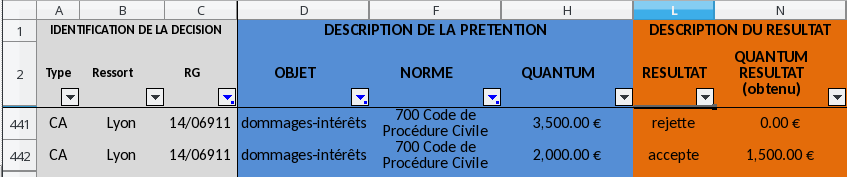
\includegraphics[width=\textwidth]{tab-annotations.png}
		\scriptsize{Les noms des champs sont sur les 2 premières lignes et les demandes sont données en exemple pour la catégorie \textit{dommages-intérêts sur le fondement de l'article 700 du code de procédure civile} (décision 14/06911 de la cour d'appel de Lyon).}
		\caption{Extrait du tableau d'annotations manuelles des demandes.} \label{tab:quanta:tab-annotations}
	\end{table}
\end{enumerate}

%Le résultat d'une phase d'annotation comprend ainsi un tableau des demandes, deux corpus de décisions $D_{c}$ et $D_{\overline{c}}$.

 Toutes les demandes du corpus $D_{c} \cup D_{\overline{c}}$  annoté manuellement, sont considérées inscrites dans le tableau des annotations manuelles. La répartition des documents d'évaluation est donnée par l'histogramme de la Figure \ref{fig:quanta:hist-repartition-docs}.  
 
 \begin{figure}[!htb]
 	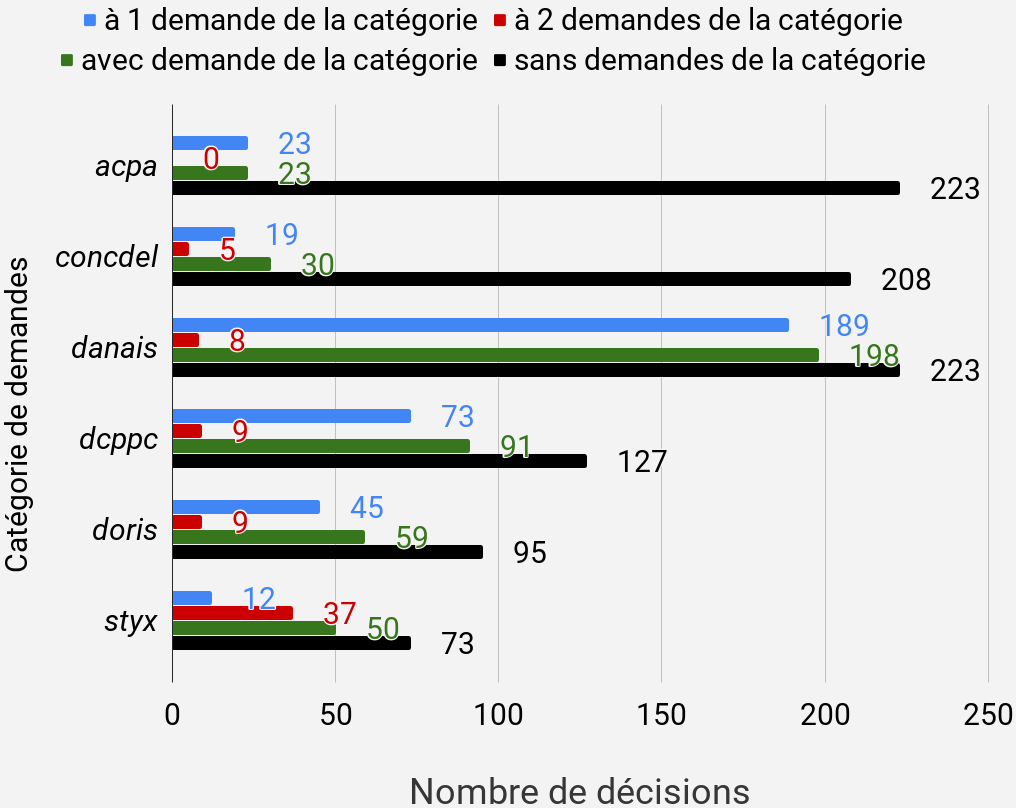
\includegraphics[width=\textwidth]{chartDataset.png}
 	\caption{Répartitions des demandes dans les documents annotées.}\label{fig:quanta:hist-repartition-docs}
 \end{figure}
 
% On remarque particulièrement que, pour toutes les catégories, les documents à une seule demande sont en général majoritaires (barres bleues).% Quelques documents ne comprenant aucune demande de la catégorie d'intérêt ont été aussi rassemblés (barres grises). 
 Il faut aussi noter que bien que l'annotation manuelle des demandes et résultats soit réalisée dans un tableau (annotation externe au contenu), elle reste une tâche très difficile. Le très faible nombre de documents annotés manuellement en témoigne. Le nombre  maximum de documents annotés pour une catégorie est seulement de 198 (barres vertes de \textit{danais}).%\textcolor{red}{[DURÉE D'ANNOTATION? QUELLE EST LA VITESSE MOYENNE D'EXTRACTION MANUELLE DES DEMANDES DANS UN DOCUMENT?]}.


%Avant l'évaluation, nous avons vérifié que les valeurs annotées existaient bel et bien dans les documents. Le calcul du taux de quanta mentionnés donne une idée de la borne supérieure de performance qu'une méthode d'extraction peut atteindre. D'autre part il faut admettre qu'il ne s'agit que d'une comparaison entre sommes d'argent juste pour savoir si une somme, de la même valeur que le quantum, est présente dans le document. Rien n'assure que la somme mentionnée est le quantum recherché.



%Les tableaux \ref{tab:quanta:mentionQd} et \ref{tab:quanta:mentionQr} donne un aperçu de la présence des valeurs de quanta dans les documents annotés, ainsi que leurs occurrences dans les différentes sections Litige, Motifs, et Dispositif. Les pourcentages ne sont calculés que pour les valeurs non nulles car les valeurs nulles ne sont généralement pas mentionnées. Un quantum demandé est noté nul si l'annotateur n'a pas trouvé sa valeur dans le document. Un quantum accordé est noté nul lorsque la demande est rejeté ou si la valeur n'est pas identifiable dans le document.
%
% Il est évident qu'en général, lorsqu'un quanta est non nul, sa valeur est identifiable dans le document. Sauf exception faite de quelques quanta qui sont calculés sur la base de valeurs mentionnées. Les taux d'occurrence des valeurs de quanta dans les diverses sections, renforce notre hypothèse selon laquelle il est possible de n'extraire les quanta demandés uniquement dans la section Litige, et les quanta accordés dans les sections Motifs et Dispositif. Le sectionnement préalable des documents trouve ainsi son importance. Malheureusement, la restriction de l'extraction dans une section particulière tend souvent à réduire les possibilités de retrouver le quantum qui se trouve dans une autre section. 

\subsection{Métriques d'évaluation}
\paragraph{Reconnaissance de catégories par classification}

La classification des documents est évaluée en utilisant les métriques précision (P), rappel (P), f1-mesure (F1) calculées à l'aide des nombres de vrais positifs (TP), faux positifs (FP), faux négatifs (FN) comme suit:
\[P = \frac{TP}{TP+FP}; R = \frac{TP}{TP+FN}; F1 = 2 \times \frac{P \times R}{P + R}\]

\paragraph{Extraction des attributs des paires demande-résultat}
 Nous évaluons les approches proposées sur l'extraction de 3 données: le quantum demandé $q_d$, le sens du résultat $s_r$ et le quantum obtenu $q_r$. Une demande est donc un triplet $(q_d, s_r, q_r)$. Il est possible d'évaluer le système pour un sous-ensemble $x$ de ce triplet sur les demandes extraites d'un corpus annotées $D$ de test. Nous utilisons les métriques traditionnellement employées en extraction d'information: la précision (Eq. \ref{eq:quanta:precisiondmd}), le rappel (Eq. \ref{eq:quanta:recalldmd}), et la F1-mesure (Eq. \ref{eq:quanta:f1dmd}). 
 \begin{equation}
 Precision_{c,x,D} = \frac{TP_{c,x,D}}{TP_{c,x,D} + FP_{c,x,D}}  \label{eq:quanta:precisiondmd}
\end{equation}

\begin{equation}
Rappel_{c,x,D} = \frac{TP_{c,x,D}}{TP_{c,x,D} + FN_{c,x,D}} \label{eq:quanta:recalldmd}
\end{equation}

\begin{equation}
F1_{c,x,D} =2 \times \frac{Precision_{c,x,D} \times Rappel_{c,x,D}}{Precision_{c,x,D} + Rappel_{c,x,D}} \label{eq:quanta:f1dmd}
\end{equation}

Ces mesures sont définies à partir des nombres de vrais positifs ($TP$), faux positifs ($FP$) et faux négatifs ($FN$). Au niveau d'un document $d$:
\begin{itemize}
\item le nombre de vrais positifs $TP_{c, x, d}$ est le nombre de demandes extraites de $d$ par le système, qui sont effectivement de la catégorie $c$ ;
\item le nombre de faux positifs $FP_{c, x, d}$ est le nombre de demandes extraites de $d$ par le système, mais qui ne sont pas des demandes de $c$ (demandes en trop);
\item le nombre de faux négatifs $FP_{c, x, d}$ est le nombre de demandes annotées comme étant de $c$ mais qui n'ont pas pu être extraites par le système (demandes manquées).
\end{itemize}

Au niveau d'un corpus d'évaluation $D$, ces métriques sont sommées: 
\[TP_{c,x,D} = \sum\limits_{d \in D} TP_{c,x,d}; FP_{c,x,D} = \sum\limits_{d \in D} FP_{c,x,d}; FN_{c,x,D} = \sum\limits_{d \in D} FN_{c,x,d}\].

Une donnée observée (par exemple \og 3 000 \euro \fg) est bien extraite automatiquement si sa valeur (le nombre $3000$) correspond à celle du quantum annoté dans le tableau. Nous considérons que les unités monétaires, entre les quanta extraits et ceux manuellement annotés, sont égales.

%La définition de la qualité d'une donnée extraite reste la question fondamentale de l'évaluation. Durant l'annotation, les données sont reportées dans le tableau sous une forme qui peut être différente de la mention dans le document. Par exemple,  La valeur observée et la valeur reportée restent néanmoins égales. Il est donc nécessaire de ne comparer que les valeurs. Pour le sens du résultat, la valeur est catégorique, et par conséquent, facilement comparable. En effet, il suffit de comparer les labels. Par contre, les quanta sont des sommes d'argent i.e. des quantités à valeur et unité monétaire. Pour simplifier, nous avons considéré que l'unité est la même pour les données extraites et annotées pour un même document. Pour obtenir la valeur, nous ramenons la mention extraite à un nombre décimal. Le symbole de la décimale étant la virgule (\og , \fg) en Français, il suffit d'éliminer, de la somme d'argent, tous les caractères différents des chiffres et de la virgule; puis remplacer cette dernière par un point. Par exemple, la valeur de \og 3 000 \euro \fg est $3000$, celle de \og 265 ' 550 , 83 euros \fg est $265550.83$ ).



\subsection{Détection des catégories par classification}
Les implémentations de la bibliothèque Weka \citep{frank2016weka} ont permis d'utilisé plusieurs modèles de classification: le modèle Bayésien naïf (NB), l'arbre de décision (J48), les k-plus-proches-voisins (KNN), et le SVM.
 A chaque entraînement, s'exécute une sélection de modèle par validation croisée sur les données d'entraînement. Elle a pour but de sélectionner la métrique locale et la métrique globale appropriée. Les résultats obtenus par 5-\textit{folds} validation croisée sont présentés sur le tableau \ref{tab:quanta:resultat-detect-cat}.  
 
\begin{table}[!h]
	\scriptsize
	\centering
	\begin{tabular}{l|ccc|ccc|ccc|ccc}
		\hline\noalign{\smallskip}
		&   \multicolumn{3}{|c|}{NB}    &    \multicolumn{3}{|c|}{J48}   &  \multicolumn{3}{|c|}{KNN}  & \multicolumn{3}{|c}{SVM}     \\       
		\noalign{\smallskip}
		\hline
		\noalign{\smallskip}
		%Categorie  
		& P     & R     & F1    & P     & R     & F1    & P     & R     & F1    & P     & R     & F1    \\        
		\noalign{\smallskip}
		\hline
		\noalign{\smallskip}
		acpa    & 1.0 & 1.0 & 1.0 & 0.996 & 0.955 & 0.972 & 1.0 & 1.0 & 1.0 & 0.996 & 0.955 & 0.972 \\
		concdel & 1.0 & 1.0 & 1.0 & 1.0 & 1.0 & 1.0 & 1.0 & 1.0 & 1.0 & 0.995 & 0.967 & 0.979 \\
		danais  & 0.988 & 0.989 & 0.988 & 0.996 & 0.995 & 0.995 & 0.995 & 0.995 & 0.995 & 0.993 & 0.993 & 0.993 \\
		dcppc   & 1.0 & 1.0 & 1.0 & 1.0 & 1.0 & 1.0 & 1.0 & 1.0 & 1.0 & 1.0 & 1.0 & 1.0 \\
		doris   & 1.0 & 1.0 & 1.0 & 1.0 & 1.0 & 1.0 & 1.0 & 1.0 & 1.0 & 1.0 & 1.0 & 1.0 \\
		styx    & 1.0 & 1.0 & 1.0 & 0.984 & 0.983 & 0.983 & 1.0 & 1.0 & 1.0 & 1.0 & 1.0 & 1.0 \\
		\hline
	\end{tabular}
(P= Précision, R=Rappel, F1 = F1-mesure)
	\caption{Résultats d'une 5-\textit{fold} validation croisée pour la détection de catégories }\label{tab:quanta:resultat-detect-cat}
\end{table}

D'après les résultats, la tâche 1 est relativement aisée pour les algorithmes traditionnels qui détectent parfaitement la présence ou non d'une catégorie dans les documents. Par conséquent, pour toute catégorie $c$, les résultats de l'extraction, dans la suite, ne sont discutés que pour les documents de $c$, car, grâce à l'efficacité de la phase de classification, aucun document de $\overline{c}$ ne sera traité par la phase d'extraction.

\subsection{Extraction de données des paires demandes-résultats}
Les scores des termes-clés candidats étant normalisés, si on sélectionne les termes dont les scores sont supérieurs à un seuil fixé, on remarque que chaque métrique d'extraction a un niveau d'efficacité différent entre les catégories de demande (Tableau \ref{tab:quanta:compareGW} avec 0.5 comme  seuil fixé). 

\begin{table}[!htb]
	\centering \scriptsize
	\begin{tabular}{|c|c|c|c|c|c|c|c|}
		\hline
		& \textit{acpa} & \textit{concdel} & \textit{danais} & \textit{dcppc} & \textit{doris} & \textit{styx} & \textbf{Moyenne} \\ \hline
		$bidf$ & 37.33 & 32.73 & 23.96 & 20.46 & 8.08 & 28.43 & 25.17 \\ \hline
		$\chi^2$ & \textbf{54.55} & 25.88 & 43.97 & 28.35 & 13.11 & 52.73 & 36.43 \\ \hline
		$dbidf$ & 37.58 & 24.63 & \textbf{56.25} & \textbf{29.06} & 11.58 & 52.73 & 35.31 \\ \hline
		$\Delta_{DF}$ & \textbf{54.55} & 25.55 & 48.16 & 28.1 & \textbf{19.64} & 52.73 & \textbf{38.12} \\ \hline
		$dsidf$ & 37.58 & 25.25 & \textbf{56.42} & 26.05 & 8.72 & \textbf{53.46} & 34.58 \\ \hline
		$gss$ & \textbf{54.55} & 25.11 & 48.16 & 28.1 & \textbf{19.64} & 52.73 & \textbf{38.05} \\ \hline
		$idf$ & 38.78 & \textbf{32.73} & 22.31 & 20.53 & 8.27 & 25.22 & 24.64 \\ \hline
		$ig$ & 4 & 12.4 & 45.21 & 14.99 & 16.74 & 51.13 & 24.08 \\ \hline
		$marascuilo$ & \textbf{54.55} & 23.65 & 43.97 & 26.67 & 17.91 & 52.73 & 36.58 \\ \hline
		$ngl$ & 42.02 & 23.97 & 52.31 & 27.21 & 13.29 & 53.2 & 35.33 \\ \hline
		$pidf$ & 26.19 & 33.71 & 21.83 & 20.46 & 8.76 & 27.68 & 23.11 \\ \hline
		$rf$ & 41.11 & 33.09 & 55.72 & 28.56 & 14.93 & 51.23 & 37.44 \\ \hline
	\end{tabular}
\caption{$F1_{c,(q_d, s_r, q_r), D_c}$ moyenne pour une 5-\textit{fold} validation croisée pour chaque métrique de sélection de termes pour un seuil égal à $0.5$} \label{tab:quanta:compareGW}
\end{table}

Par conséquent, la métrique et le seuil doivent être bien sélectionnés en fonction de la catégorie de demandes traitée. En choisissant, pour ces méta-paramètres, les valeurs qui donnent les meilleurs performances d'extraction sur la base d'apprentissage, les résultats suivants sont observés (Tableau \ref{tab:quanta:resultDetailExtraction}).
 

\begin{table}[!htb]
	\centering \scriptsize
	\begin{tabular}{l|l|l|llll|llll}
			\hline\noalign{\smallskip}
		&                 &                       &          \multicolumn{4}{|c|}{Données d'entraînement}      &      \multicolumn{4}{|c}{Données de test}       \\ \hline
		$c$ & Données & $\vert V_c \vert$ & P     & R     & F1                       & \%Docs & P     & R     & F1              & \%Docs \\ \hline
		\multirow{5}{*}{\textit{acpa}}  & $q_d$ & 1 & 86.4 & 56.37 & 68.13 & 56.37 & 68.33 & 54 & 58.99 & 46 \\
		& $q_r$ & 1 & 100 & 65.09 & 78.74 & 65.09 & 93.33 & 63 & 71.43 & 55 \\
		& $s_r$ & 1 & 100 & 65.09 & 78.74 & 65.09 & 93.33 & 63 & 71.43 & 55 \\
		& $(s_r, q_r)$ & 1 & 100 & 65.09 & 78.74 & 65.09 & 93.33 & 63 & 71.43 & 55 \\
		& $(q_d,s_r, q_r)$ & 1 & 86.4 & 56.37 & 68.13 & 56.37 & 68.33 & 54 & 58.99 & 46 \\ \hline
		\multirow{5}{*}{\textit{concdel}}  & $q_d$ & 26 & 49.33 & 44.02 & 45.31 & 24.17 & 73.2 & 29.72 & 33.29 & 26.67 \\
		& $q_r$ & 26 & 48.3 & 42.66 & 44.1 & 22.5 & 75.73 & 28.89 & 34.3 & 26.67 \\
		& $s_r$ & 26 & 46.52 & 40.89 & 42.36 & 22.5 & 74.93 & 26.39 & 33.09 & 26.67 \\
		& $(s_r, q_r)$ & 26 & 46.52 & 40.89 & 42.36 & 22.5 & 74.93 & 26.39 & 33.09 & 26.67 \\
		& $(q_d,s_r, q_r)$ & 26 & 42.43 & 37.41 & 38.68 & 20.83 & 68.27 & 23.06 & 28.65 & 23.33 \\ \hline
		\multirow{5}{*}{\textit{danais}} & $q_d$ & 37 & 77.71 & 48.71 & 59.68 & 37.3 & 79.25 & 47.5 & 59 & 37.3 \\
		& $q_r$ & 37 & 77.68 & 48.71 & 59.67 & 37.03 & 77.78 & 46.46 & 57.79 & 36.22 \\
		& $s_r$ & 37 & 77.05 & 48.33 & 59.19 & 37.03 & 77.78 & 46.46 & 57.79 & 36.22 \\
		& $(s_r, q_r)$ & 37 & 77.05 & 48.33 & 59.19 & 37.03 & 77.78 & 46.46 & 57.79 & 36.22 \\
		& $(q_d,s_r, q_r)$ & 37 & 74.45 & 46.65 & 57.16 & 35.81 & 74.41 & 44.38 & 55.23 & 34.59 \\ \hline
		\multirow{5}{*}{\textit{dcppc}}   & $q_d$ & 35 & 45.71 & 36.64 & 40.66 & 34.05 & 44.64 & 40.73 & 41.75 & 31.4 \\
		& $q_r$ & 35 & 78.99 & 63.21 & 70.2 & 59.33 & 75.48 & 64.51 & 68.41 & 53.82 \\
		& $s_r$ & 35 & 84.73 & 67.85 & 75.33 & 63.24 & 81.21 & 69.14 & 73.51 & 57.43 \\
		& $(s_r, q_r)$ & 35 & 78.99 & 63.21 & 70.2 & 59.33 & 75.48 & 64.51 & 68.41 & 53.82 \\
		& $(q_d,s_r, q_r)$ & 35 & 34.2 & 27.39 & 30.41 & 28.03 & 31.66 & 28.55 & 29.41 & 25.37 \\ \hline
		\multirow{5}{*}{\textit{doris}}  & $q_d$ & 8 & 31.98 & 35.76 & 32.94 & 7.75 & 37.48 & 35.9 & 36.63 & 7.12 \\
		& $q_r$ & 8 & 35.73 & 39.72 & 36.69 & 8.63 & 39.43 & 38.47 & 38.89 & 7.12 \\
		& $s_r$ & 8 & 35.06 & 39.56 & 36.24 & 9.06 & 42.91 & 41.44 & 42.12 & 8.94 \\
		& $(s_r, q_r)$ & 8 & 32.61 & 36.16 & 33.45 & 8.2 & 38.14 & 37.04 & 37.54 & 7.12 \\
		& $(q_d,s_r, q_r)$ & 8 & 24.48 & 27.16 & 25.13 & 5.61 & 29.7 & 28.53 & 29.08 & 7.12 \\ \hline
		\multirow{5}{*}{\textit{styx}} & $q_d$ & 4 & 69.34 & 59.55 & 64.04 & 33.5 & 69.3 & 59.49 & 63.61 & 32 \\
		& $q_r$ & 4 & 75.87 & 65.17 & 70.08 & 31.5 & 74.86 & 64.08 & 68.63 & 28 \\
		& $s_r$ & 4 & 75.87 & 65.17 & 70.08 & 31.5 & 74.86 & 64.08 & 68.63 & 28 \\
		& $(s_r, q_r)$ & 4 & 75.87 & 65.17 & 70.08 & 31.5 & 74.86 & 64.08 & 68.63 & 28 \\
		& $(q_d,s_r, q_r)$ & 4 & 57.61 & 49.44 & 53.19 & 25.5 & 57.24 & 48.36 & 52.08 & 24  \\
			\hline\noalign{\smallskip}
	\end{tabular}

P: précision, R: rappel, F1: F1-mesure
	
\%Docs: proportion de documents dont l'ensemble des données extraites est égale à l'attendu (documents parfaitement traités)

$\vert V_c \vert$: nombre moyen de termes-clés identifiés pour la catégorie $c$
\caption{Résultats détaillés pour l'extraction des données avec sélection automatique de la méthode d'extraction des termes-clés} \label{tab:quanta:resultDetailExtraction}
\end{table}


Ces résultats détaillés font remarquer que les attributs, pris individuellement, présentent d'assez bonnes performances. Cependant, la mise en correspondance des attributs (triplet $(q_d,s_r, q_r)$) peine toujours à montrer des performances du même rang. On remarque néanmoins que les mesures-F1 $(q_d,s_r, q_r)$ sont proches de celles des attributs qui présentent le plus de difficulté. L'échec de l'extraction de ces attributs est une des principales causes des performances observées pour la liaison des attributs de paires similaires demande-résultat. Par ailleurs, les données sur le résultat, $s_r$ et $q_r$, sont en générale plus faciles à extraire que le quantum demandé $q_d$. Il est aussi bien de noter qu'une plus grande quantité d'exemples annotés de documents ne semble pas être la garantie d'une meilleure extraction. On remarque en effet que les meilleures performances sont obtenues pour la catégorie disposant du plus faible nombre d'exemples annotés (\textit{acpa}) avec en moyenne un seul terme-clé appris. %Dans la suite, divers aspects sont décrits pour expliquer les raisons des limites de l'approche proposée.

\subsection{Analyse des erreurs}

En extraction d'éléments structurés, on retrouve trois types d'erreurs \citep{yang2016jointEntityEvt}: les données manquées (faux négatifs), les données en plus des attendues (faux positifs), et les mauvaises classifications (confusions). La confusion n'est pas discutée ici car les annotations ne sont faites que pour une seule classe. %Les confusions sont évitées dans l'approche proposée par la détection préalable des catégories par classification et l'extraction restreinte à une seule catégorie à la fois. 

Etant donné que la précision est en général supérieure au rappel, il est certain que les erreurs sont majoritairement dues aux données manquées comme le confirme le Tableau \ref{tab:quanta:types_erreurs}. 

\begin{table}[!htb]
	\centering\scriptsize
	\begin{tabular}{|c|c|c|c|c|}
		\hline
		      &    \multicolumn{2}{|c|}{Données d'entraînement}      &      \multicolumn{2}{|c|}{Données de test}       \\ \hline
		& \textbf{\%erreurs FP} & \textbf{\%erreurs FN} & \textbf{\%erreurs FP} & \textbf{\%erreurs FN} \\ \hline
		$q_d$            & 36.90                 & 63.10                 & 36.52                 & 63.48                 \\ \hline
		$q_r$            & 32.30                 & 67.70                 & 34.32                 & 65.68                 \\ \hline
		$s_r$            & 31.72                 & 68.28                 & 34.11                 & 65.89                 \\ \hline
		$(s_r, q_r)$     & 32.32                 & 67.68                 & 34.39                 & 65.61                 \\ \hline
		$(q_d,s_r, q_r)$ & 37.77                 & 62.23                 & 37.72                 & 62.28                 \\ \hline
	\end{tabular}
\caption{Types et taux d'erreurs (pourcentage en moyenne sur les 6 catégories de demandes)} \label{tab:quanta:types_erreurs}
\end{table}

Trois raisons peuvent expliquer le fait que  peu de données attendues soient extraites. Premièrement, certaines valeurs d'attributs ne sont pas mentionnées dans les sections Litige et Dispositif utilisées (pourcentage inférieurs à 100 dans les Tableaux \ref{tab:quanta:mentionQd} et \ref{tab:quanta:mentionQr} comme par exemple les quanta résultat de \textit{doris} plus présents dans la section Motifs que dans le Dispositif).

\begin{table}[!htb]
	\scriptsize
	\begin{tabular}{|l|l|l|l|l|l|l|}
		\hline
		%\textbf{Catégorie}
		& \textbf{\#$q_d$} & \textbf{\#$q_d\neq NUL$} & \textbf{\# dans doc.} & \textbf{\# dans Litige} & \textbf{\# dans Motifs} & \textbf{\# dans Dispositif} \\ \hline
		acpa               & 23                   & 16                                           & 16 (100\%)                   & 16 (100\%)              & 9 (56.25\%)             & 5 (31.25\%)                 \\ \hline
		concdel            & 58                   & 56                                           & 55 (98.21\%)                 & 55 (98.21\%)            & 7 (12.5\%)              & 2 (3.57\%)                  \\ \hline
		danais             & 208                  & 182                                          & 182 (100\%)                  & 179(100\%)              & 39 (21.43\%)            & 23 (12.64\%)                \\ \hline
		dcppc              & 126                  & 126                                          & 122 (96.83\%)                & 109 (86.51\%)           & 71 (56.35\%)            & 65 (51.59\%)                \\ \hline
		doris              & 94                   & 83                                           & 83 (100\%)                   & 82 (98.80\%)            & 21 (25.30)\%            & 6 (7.23\%)                  \\ \hline
		styx               & 89                   & 86                                           & 86 (100\%)                   & 86 (100\%)              & 12 (13.95\%)            & 9 (10.47\%)                 \\ \hline
	\end{tabular}
	\textit{Les pourcentages ne sont calculés que pour les valeurs non nulles}
	\caption{Taux de quanta demandés ($q_d$) mentionnés dans les documents annotés} \label{tab:quanta:mentionQd}
\end{table}

\begin{table}[!htb]
	\scriptsize
	\begin{tabular}{|l|l|l|l|l|l|l|}
		\hline
		%\textbf{Catégorie}
		& \textbf{\# $q_r$} & \textbf{\# $q_r\neq NUL$} & \textbf{\# dans doc.} & \textbf{\# dans Litige} & \textbf{\# dans Motifs} & \textbf{\# dans Dispositif} \\ \hline
		acpa               & 23                & 6                       & 6 (100\%)             & 3 (50\%)                & 6 (100\%)               & 5 (83.33\%)                 \\ \hline
		concdel            & 58                & 8                       & 8 (100\%)             & 2 (25\%)                & 8 (100\%)               & 6 (75\%)                    \\ \hline
		danais             & 208               & 23                      & 23 (100\%)            & 15 (65.22\%)            & 22 (95.65\%)            & 20 (86.96\%)                \\ \hline
		dcppc              & 126               & 76                      & 75 (98.68\%)          & 55 (72.37\%)            & 56 (73.68\%)            & 64 (84.21\%)                \\ \hline
		doris              & 94                & 44                      & 44 (100\%)            & 28 (63.64\%)            & 40 (90.91)\%            & 24 (54.55\%)                \\ \hline
		styx               & 89                & 30                      & 29 (96.67\%)          & 16 (53.33\%)            & 22 (73.33\%)            & 29 (96.67\%)                \\ \hline
	\end{tabular}
	\textit{Les pourcentages ne sont calculés que pour les valeurs non nulles}
	\caption{Taux de quanta accordés ($q_r$) mentionnés dans les documents annotés} \label{tab:quanta:mentionQr}
\end{table}

Deuxièmement, la sélection des termes-clés n'est pas parfaite (Tableau \ref{tab:quanta:exemples_termes}). D'une part, l'ensemble sélectionné ne couvre  pas toutes les situations d'expression de la catégorie (par exemple, pour la catégorie \textit{styx}, le terme \og frais irrépétibles\fg{} est souvent utilisés à la place de \og article 700 du code de procédure civile\fg{}, mais dans très peu d'exemples annotés). D'autre part, certains termes sont trop spécifiques à la base d'apprentissage (par exemple, pour la catégorie \textit{concdel}, des sommes d'argent et autres termes comme \og condamner in solidum les sociétés \fg{} apparaissent dans la liste).

\begin{table}[!htb]
		\centering\scriptsize
	\begin{tabular}{|l|p{0.8\textwidth}|}
		\hline
		\textbf{Catégorie} & \textbf{Termes-clés appris} \\ \hline
		\textit{acpa}    & amende civile                                                                                                                                                                                                                               \\ \hline
		\textit{concdel} & titre de la concurrence déloyale, somme de 15000euros à titre, réparation de son préjudice financier, payer la somme de 15000euros, condamner in solidum les sociétés, agissements constitutifs de concurrence déloyale                   \\ \hline
		\textit{danais}  & dommages et intérêts pour procédure, 32-1 du code de procédure, intérêts pour procédure abusive, titre de dommages-intérêts pour procédure, intérêts pour procédure, article 32-1 du code, dommages-intérêts pour procédure abusive         \\ \hline
		\textit{dcppc}   & admet la créance déclarée, admet la créance, passif de la procédure collective, passif de la procédure, hauteur de la somme, créance déclarée, titre chirographaire, admission de la créance, rejette la créance,                           \\ \hline
		\textit{doris}   & préjudices, abusive, condamner solidairement, solidairement, réparation du préjudice, réparation, titre de dommages et intérêts, dommages, titre de dommages, dommages et intérêts, titre de dommages-intérêts, payer aux époux, jouissance \\ \hline
		\textit{styx}    & 700 du code de procédure, article 700 du code, 700 du code, article 700, 700                                                                                                                                                                \\ \hline
	\end{tabular}
Les termes candidats sont des n-grammes de taille variant d'1 à 5 mots consécutifs
\caption{Premiers termes sélectionnés lors de la première itération de la validation croisée} \label{tab:quanta:exemples_termes}
\end{table}

Troisièmement, les expérimentations ont été réalisées sur des décisions d'appel mais les énoncés, de demande et résultat renvoyant aux décisions de jugements antérieurs, ne sont pas encore traités dans l'approche. Ces références aux décisions antérieures représentent une part importante des demandes discutées dans les décisions d'appel. Il est donc nécessaire de les intégrer explicitement dans le processus d'extraction, pour compléter les données extraites.

\section{Conclusion}
\label{sec:quanta:conclusion}
Ce chapitre décrit le problème d'extraction de données pertinentes relatives aux paires demande-résultat mentionnées dans les décisions de justice. Les divers défis relatifs à la tâche  y sont discutés en remarquant des analogies avec d'autres tâches classiques de la fouille de données textuelles. Il a été démontré la solvabilité du problème par la proposition et l'expérimentation d'une approche d'extraction basée sur l'apprentissage de la terminologie des catégories de demande et autres connaissances du domaine judiciaire telles que les motifs d'énoncés de demandes et de résultat, ainsi que leur position conventionnelle dans les documents.  Les expérimentations démontrent que l'approche permet d'extraire plus ou moins bien des demandes selon la catégorie traitée. A cause de la  forte dépendance aux subtilités de rédaction des décisions judiciaires, la méthode rencontre des limites qui ne peuvent être surmontées qu'en rendant la méthode beaucoup plus complexe qu'elle ne l'est déjà. Des approches d'apprentissage automatique sont recommandées comme perspectives. Elles devront être capables d'apprendre l'emplacement des données à extraire de manière semi-supervisée à l'aide de faibles quantités de documents annotés de grande taille.
 % INCLUDE: quanta
\chapter{Identification du Sens du Résultat par Classification}
\label{chap:sensresultat}

\section{Objectif et Motivation}
\label{sec:sensresultat:motivation}
Comme le précédent, ce chapitre est relatif à l'extraction de données sur les demandes, mais  il est question ici d'extraire uniquement le sens du résultat d'une demande connaissant sa catégorie. Cette étude est intéressante parce que le problème devient plus simple. En se passant de la localisation précise des quanta ou plus globalement des passages d'expression des demandes et résultats, l'extraction du sens du résultat peut être formulée comme une tâche de classification de documents. Nous modélisons la tâche comme une classification binaire où un algorithme est entraîné à déterminer si la demande a été rejetée (sens = rejette) ou acceptée (sens = accepte). Nous avons proposé cette modélisation sur une restriction du problème définie par les postulats \ref{postulat:sens:unedemande} et \ref{postulat:sens:sensbinaire}.

\begin{postulat}\label{postulat:sens:unedemande}
Pour toute catégorie de demande $C$, la majorité des documents ne contiennent qu'une demande de catégorie $C$. \textcolor{red}{COMMENT SAVOIR QU'UN DOCUMENT N'A QU'UNE SEULE DEMANDE? CLASSIFICATION POSSIBLE?}
%Pour toute catégorie de demande $C$, on ne considère que les décisions dans lesquelles n'apparaît qu'une seule demande de catégorie $C$. 
\end{postulat} 
Ce postulat est légitime car les statistiques sur les données labellisées de la Figure \ref{fig:quanta:hist-repartition-docs} montre bien que pour la majorité des catégories, peu de décisions contiennent plus d'une demande. On remarque néanmoins l'exception de la catégorie STYX (dommage-intérêt sur l'article 700 CPC), où dans la majorité des documents, on a plutôt 2 demandes. Cette exception peut se justifier par le fait que chaque partie fait généralement ce type de demande car elle porte sur le remboursement de frais de justice. Ce postulat présente cependant un inconvénient dû au fait que la majorité des demandes se trouvent dans des décisions à plus d'une demande. Il est donc possible de manquer un grand nombre de demandes. %On pourrait peut-être porter la classification à un modèle multi-label qui déterminera plusieurs sens à partir d'un seul document. Par exemple <SENS1, SENS2, SENS3> avec des valeurs prédéfinies sur les SENS 2 et 3 par exemple NO-DMD pour indiquer que la décision ne comprend pas de seconde ou de troisième demande.

\begin{postulat}\label{postulat:sens:sensbinaire}
Le sens du résultat est généralement binaire: accepte ou rejette.
\end{postulat} 
Ce postulat est justifié car le sens d'un résultat est pratiquement toujours une de ces deux valeurs (Figure \ref{stat-sensrst}). Les autres sens étant très rares, nous ne les considérons pas.

\begin{figure}
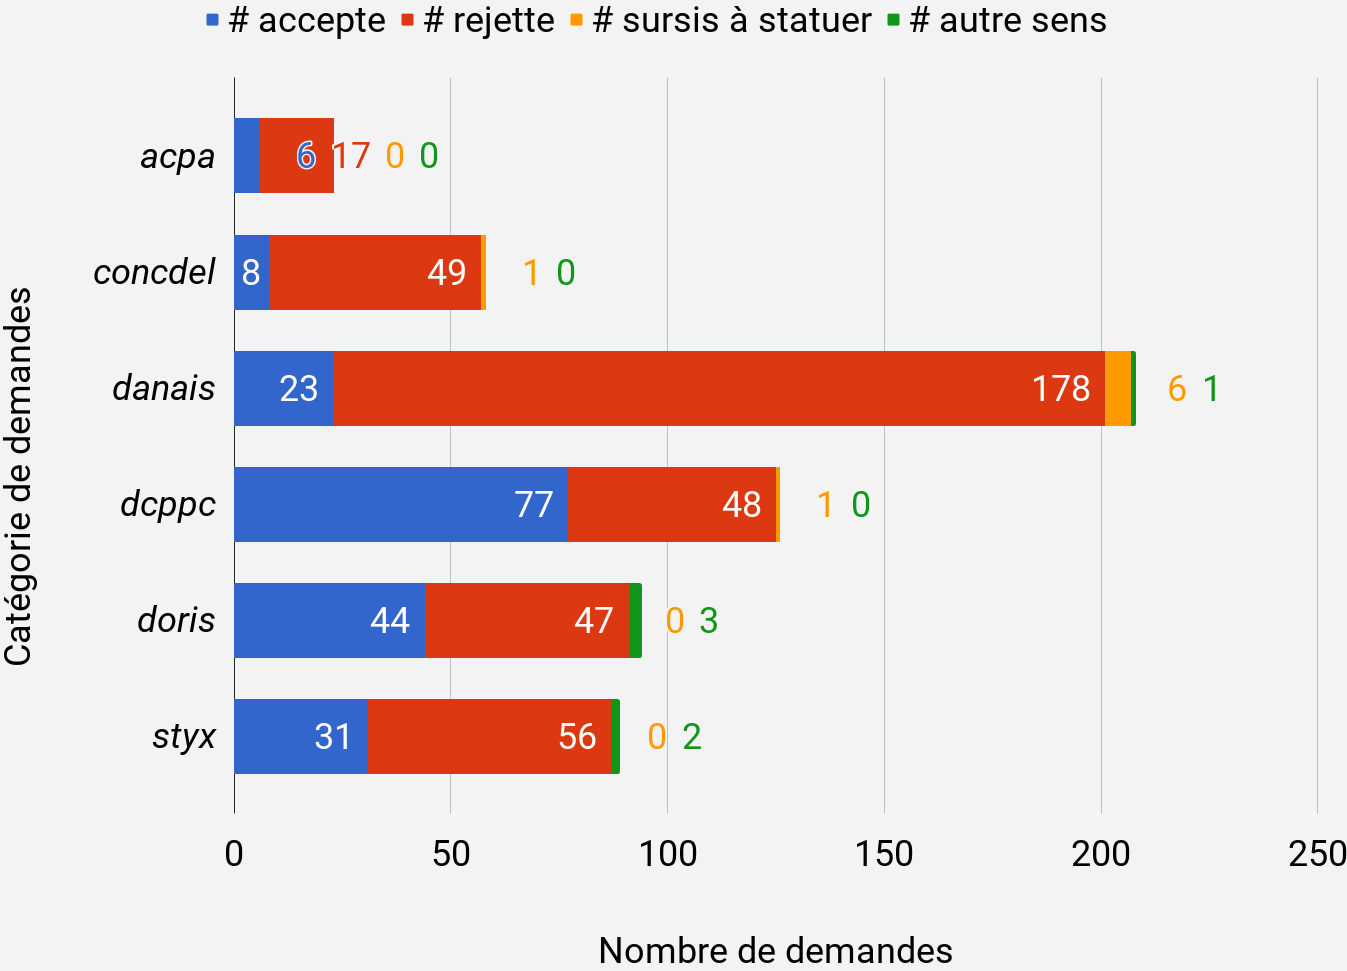
\includegraphics[width=\textwidth]{chartDistrSens.png}
\caption{Répartition des sens de résultat dans les données annotées.}\label{stat-sensrst}
\end{figure}
\section{Formulation du Problème}
\label{sec:sensresultat:probleme}

Cette étude porte sur l'analyse de l'impact de différents aspects techniques généralement appliqués dans le cadre de la classification de texte:
La représentation de texte (généralement vectorielle) faisant intervenir les notions de BagOfWord, TFIDF, poids global, poids local, matrice document-terme
La transformation de dimension a pour but de projeter le vecteur représentant un document dans un nouvel espace où généralement la distinction des classes est plus facile. Ceci est généralement effectuée en déterminant des composantes discriminantes à partir de la base d'entraînement: sélection de caractéristique, réduction matricielle, représentation vectorielle “sémantique” des documents (LatentDA, LSA, word embedding, ...)

 Cette analyse permettra de savoir s'il existe une certaine configuration permettant de déterminer le sens du résultat à une demande sans nécessairement l'avoir identifiée précisément dans le document. 


\section{Classification de Documents}
\label{sec:sensresultat:biblio_classif}

La classification de texte permet d'organiser des documents $x^{(k)}$ dans des groupes prédéfinis. Elle reçoit depuis longtemps beaucoup d'attentions. Deux choix techniques influencent principalement les performances: la représentation des textes et l'algorithme de classification. 

\subsection{Algorithmes traditionnels}
Bien que la classification de documents voit de plus en plus se développer des algorithmes propres aux textes, un grand nombre de méthodes ont été développées précédemment autour. Ces méthodes sont généralement basée sur une représentation vectorielle des textes et délimitent une frontière entre les classes dans un espace multidimensionnel. 
%NB et SVM : https://www.dropbox.com/home/Documents/to-read/term-weight?preview=Best+Terms+An+Efficient+Feature+Selection+Algorithm+for+Text+Categorization.pdf

\subsection{Etat de l'art}
Actuellement, les algorithmes NBSVM et FastText sont les plus populaires pour la classification de documents et ont les performances pour l'analyse de sentiment sont très bonnes. 

Le NBSVM \citep{wang2012nbsvm} est un classifieur binaire (classes $\lbrace -1; 1 \rbrace$) dont le principe consiste à transformer les poids $f^{(k)}$ caractéristiques $V$ des textes $x^{(k)}$, réduites à leur simple présence $\widehat{f}^{(k)}$ en réalisant leur produit élément à élément ($\overset{\sim}{f}^{(k)} = {r} \circ \widehat{f}^{(k)}$) avec le vecteur de poids $r$ du classifieurs bayésien multinomial (calculé avec le vecteur présence de caractéristique):
$r = \log \left( \frac{p/\vert\vert p \vert\vert_1}{q / \vert\vert q \vert\vert_1}\right)
\text{ avec } p=\alpha + \sum\limits_{k:y^{(k)}=1}{f}^{(k)}$, $q=\alpha + \sum\limits_{k:y^{(k)}=-1}{f}^{(k)}$. L'ensemble des caractéristiques $V$ est constitué de n-grammes de mots. Le nouveau vecteur issu de ce produit représente le texte ($x^{(k)} = \overset{\sim}{f}^{(k)}$) en entrée d'un SVM classique. La classe de $x^{(k)}$ est prédite par : $y^{(k)} = sign(\mathbf{w}^Tx^{(k)} + b)$, $\mathbf{w}$ et $b$ étant appris lors de l'entrainement du SVM. Une interpolation  entre le bayésien multinomial et le SVM est nécessaire pour assurer la robustesse du NBSVM et des performances excellentes pour toute tâche de classification de documents; les poids $\mathbf{w}$ sont réajustés par le model $\mathbf{w'} = (1 - \beta) \overline{w} + \beta \mathbf{w}$, où $\overline{w} = \vert\vert \mathbf{w}\vert\vert_1 / \vert V \vert$ et $\beta \in \left[0; 1] \right.$. 
  
 FastText \citep{grave2017fasttextcls}, quant à lui, est un modèle de réseau de neurones dont l'architecture est semblable à celle de la variante CBOW de la méthode de plongement sémantique Word2Vec dans laquelle le mot du milieu a été remplacé par le label de la classe du texte et au dessus de laquelle la fonction softmax $f(z) = \left[ \frac{e^{z_j}}{\sum\limits_{k=1}^K e^{z_k}} \right]_{\forall j \in \lbrace 1, ..., K \rbrace} $ est rajoutée pour réaliser la classification à partir de la représentation distribuée du texte. La phase d''entraînement consiste à minimiser la fonction objectif $-\frac{1}{N}y_n \cdot \sum\limits_{n=1}^N y_n \cdot \log{f(B\cdot A\cdot x_n)}$ qui estime la distribution de probabilité des classes.

Le fonctionnement de ces deux méthodes intègrent leur propre représentation, contrairement aux algorithmes traitant des vecteurs comme le SVM. Il existe un très grand nombre de schémas de représentations vectorielles des documents.

NBSVM et Fastext ont démontré une bonne robustesse et et des performances excellentes dans le cas de divers tâches de classification: courtes expressions, longs documents, thème, classification subjective (genre), classification de sentiment (positif, neutre, négatif), ... Mais nous voulons déjà savoir comment les algorithmes populaires se comportent sur notre tâche d'identification de la polarité du résultat d'une demande pour une catégorie bien définie. La particularité ici est que la tâche porte sur une demande en particulier parmi les nombreuses que compte le document, des données en faible nombre annotés (23 à 189 documents), une annotation en général déséquilibrée entre les classes (risque d'ignorer une classe très faiblement représenté dans le jeu d'entrainement, par exemple 21 "accepte" contre 166 "rejette").

\subsection{Classification des décisions de justice}

\section{La Regression PLS et ses extensions}
\label{sec:sensresultat:pls}
\textcolor{red}{Justification: Pourquoi le PLS?:}
%https://link.springer.com/content/pdf/10.1007\%2FBF02174528.pdf, 
%https://www.stat4decision.com/fr/regression-pls/
La regression PLS est une méthode de regression avec laquelle l'on tente d'expliquer une ou plusieurs variables Y (dite dépendantes) par des variables $X=x_1,x_2,...,x_p$ (dites explicatives). Elle consiste principalement à transformer les variables explicatives en un nombre réduit de composantes principales orthogonales $t_1, t_2, ..., t_h$. Les composantes $t_h$ sont construites étapes par étapes en applicant l'algorithme du PLS de façon récurrente sur les données mal prédites (résidus). Plus précisément, à chaque itération $h$, la composante $t_h$ est calculée par la formule $t_h = w_{h1} x_1 + \cdots + w_{hj} x_j + \cdots + w_{hp} x_p$. 

Malgré quelques faiblesses comme celles liées au choix du nombre de composantes, à la complexité des sorties et la linéarité du modèle, la regression PLS présente quelques atouts qui ont notamment de l'intérêt dans notre cas de figure. Par exemple, le PLS gère assez bien la forte dispropotion entre le nombre de variables explicatives et le nombre d'observations, lorsque ce dernier est faible comme on peut l'observer dans nos données (faible quantité de données d'apprentissage). Nous avons aussi la prise en compte de la multicolinéarité qui peut exister entre les variables explicatives, notamment quand celles-ci sont associées aux mots/termes souvent cooccurrents de nos documents.

Il est intéressant de noter la floraison d'extensions proposées pour répondre aux différentes limites du PLS. Notamment, nous pouvons citer la "\textit{sparse}" PLS introduite pour palier à la "\textit{sparsité}" et la colinéarité des variables explicatives [?], la PLS non-linéaire proposée pour les cas de données non-linéairement séparables [?], ou encore la PLS discriminante combinant la régression PLS et l'analyse discriminante [?]. Nos nous sommes intéressés à deux extensions particulières: la régression Gini-PLS \citep{mussard2018ginipls} dont l'intérêt est de réduire la sensibilité aux valeurs aberrantes des variables, et la regression Logit-PLS \citep{tenenhaus2005logitpls}  combinant la regression logistique et la PLS.
\subsection{Gini-PLS}
Cette méthode élimine la sensibilité du PLS aux valeurs extrêmes en remplaçant la covariance $cov(x_j, y)$ par la covariance de Gini $cog(y; x_j) := cov(y; R(x_j))$ pour l'estimation des résidus $u_{(h)j}$ et des poids $w_{hj}$ \citep{mussard2018ginipls}.


\subsection{Logit-PLS}
Dans cette approche, $\forall j > 1$, les $w_{hj} $ sont les coefficients de la régression logistique de $y$ sur les composantes $t_1, ..., t_{h-1}, u_{(h-1)j}$ \cite{tenenhaus2005logitpls}.

\subsection{Gini-Logit-PLS}
Cette approche combine la covariance Gini pour $u_{(h)j}$ et le coefficient Logit pour les $w_{hj}$.

\section{Expérimentations et résultats}
\label{sec:sensresultat:experimentations}
\subsection{Protocole d'évaluation}
Nous discutons ici les performances de divers algorithmes populaires et l'impact de la quantité et du déséquilibre des données, de la restriction à des passages en particulier, aisin que leur capacité à faire abstraction des autres demandes du document. Deux métriques d'évaluation sont utilisées: la précision et la F1-mesure. Du fait du déséquilibre entre les classes, la moyenne des performances sur les deux classe sera micro (agrégation de la contribution individuelle de chaque classe: $F1_{moyenne} = (F1({accepte}) + F1({rejette})) / 2$).

Les données utilisées sont les mêmes que celles du chapitre précédent. Nous avons seulement fait une restriction sur les documents n'ayant qu'une seule demande annotée pour la catégorie considérée. Le déséquilibre entre les classes est illustrée par la figure \ref{fig:sensresultat:stat-1dmd}. En effet, la demande est plus souvent rejetée qu'acceptée pour les catégorie ACPA, CONCDEL, DANAIS et STYX. Le contraire est observé pour DCPPC et DORIS.
\begin{figure}[htb]
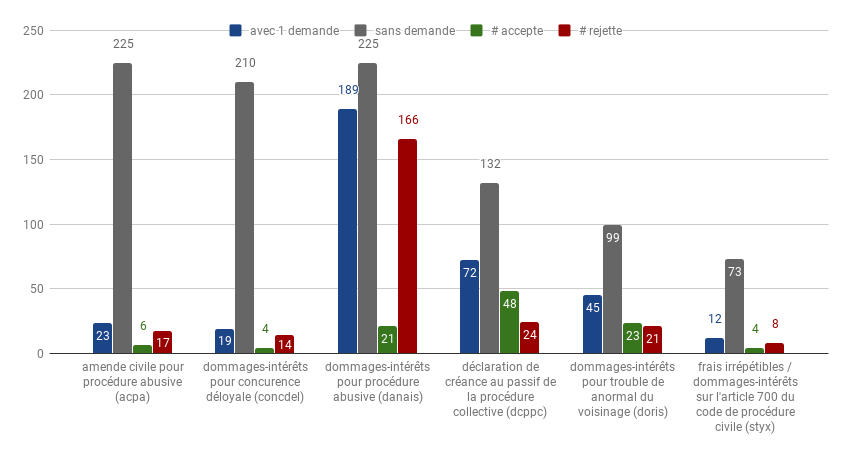
\includegraphics[width=\textwidth]{chartDataset1dmd.png}
\caption{Répartition des documents à une demande de la catégorie considérée.}\label{fig:sensresultat:stat-1dmd}
\end{figure}

\subsection{Performances observées}

\begin{table}
\scriptsize
\begin{tabular}{|l|l|l|l|l|l|l|l|l|}
\hline
\textbf{Cat. Dmd.} & \textbf{Algo.} & \textbf{Préc.}   & \textbf{Préc. équi.} & \textbf{err-0} & \textbf{err-1} & \textbf{f1-0}  & \textbf{f1-1}  & \textbf{f1-macro-avg} \\ \hline
\textbf{dcppc}       & nbsvm      & 0.875 & 0.812        & 0.375 & 0     & 0.752 & 0.916 & \textbf{0.834}        \\ \hline
danais      & fasttext   & \textbf{0.888} & 0.5          & 1     & 0     & 0     & 0.941 & 0.47         \\ \hline
danais      & nbsvm      & 0.888 & 0.5          & 0     & 1     & 0.941 & 0     & 0.47         \\ \hline
concdel     & fasttext   & 0.775 & 0.5          & 1     & 0     & 0     & 0.873 & 0.437        \\ \hline
concdel     & nbsvm      & 0.775 & 0.5          & 0     & 1     & 0.873 & 0     & 0.437        \\ \hline
acpa        & fasttext   & 0.745 & 0.5          & 1     & 0     & 0     & 0.853 & 0.426        \\ \hline
acpa        & nbsvm      & 0.745 & 0.5          & 0     & 1     & 0.853 & 0     & 0.426        \\ \hline
doris       & nbsvm      & 0.5   & 0.492        & 0.85  & 0.167 & 0.174 & 0.63  & 0.402        \\ \hline
dcppc       & fasttext   & 0.667 & 0.5          & 0     & 1     & 0.8   & 0     & 0.4          \\ \hline
styx        & fasttext   & 0.667 & 0.5          & 1     & 0     & 0     & 0.8   & 0.4          \\ \hline
styx        & nbsvm      & 0.667 & 0.5          & 0     & 1     & 0.8   & 0     & 0.4          \\ \hline
doris       & fasttext   & 0.523 & 0.5          & 0     & 1     & 0.686 & 0     & 0.343        \\ \hline
\end{tabular}
0 == accepte

1 == rejette

\caption{Performances des classifieurs pour l'identification du sens du résultat} \label{tab:sensresultat:perf-base}
\end{table}



\subsection{Discussions}
\subsubsection{Déséquilibre des classes}
\subsubsection{Quantités de données annotées}
\subsubsection{Restriction à une région particulière du document}
\subsubsection{Représentation des documents}

\section{Conclusion}
\label{sec:sensresultat:conclusion} % INCLUDE: sensresultat
 \chapter{Modélisation des Circonstances Factuelles}
\label{chap:similarite}

%\epigraph{Le plus important, c'est d'avoir un langage métaphorique ; car c'est le seul mérite qu'on ne puisse emprunter à un autre et qui dénote un esprit naturellement bien doué ; vu que, bien placer une métaphore, c'est avoir égard aux rapports de ressemblance.}{Aristote, Poétique}
% 

\section{Introduction}
\label{sec:similarite:introduction}
Les circonstances factuelles sont les types de faits ou contextes possibles dans lesquels une catégorie de demande peut être formulée. Les analyses descriptives ou prédictives ne prennent sens que lorsqu'elles sont appliquées à un ensemble de décisions aux circonstances similaires. Par exemple, il serait imprudent de considérer toutes les décisions pour prédire les chances d'acceptation d'une demande de dommages-intérêts fondée sur l'\og article 700 du code de procédure civile \fg{} en cas de trouble de voisinage. Les taux d'acceptation ou de rejet peuvent être différents entre des affaires de licenciement et celles portant sur les troubles anormaux du voisinage, et même plus spécifiquement entre les troubles de voisinage entre particulier et entreprises (par exemple: chantier de construction), ou simplement entre particuliers (par exemple: troubles sonores). Il serait préférable de travailler uniquement avec des décisions similaires à la situation d'intérêt. L'identification des circonstances factuelles devient donc indispensable. Malheureusement, les faits et leur catégorisation sont extrêmement diversifiés et indénombrables.Annoter manuellement des échantillons de décisions est impossible pour chaque circonstance potentielle afin de résoudre ce problème par classification supervisée. Il est donc plus intéressant d'adopter une approche non-supervisée capable modéliser les circonstances factuelles à partir d'un corpus de documents d'une même catégorie de demande. Plus précisément, l’objectif est donc de regrouper ensemble les décisions qui traitent de problèmes similaires. La tâche peut être formulée comme une tâche de regroupement non-supervisé (\textit{clustering}).  Les objectifs de ce chapitre sont d'expérimenter des algorithmes  de \textit{clustrering} et des métriques de similarité, et de démontrer que l'apprentissage d'une distance de similarité entre documents d'une même catégorie de demande permet d'obtenir un meilleur clustering.

%\section{Formulation du Problème}
%\label{sec:similarite:probleme}

\section{Regroupement non-supervisé de documents}
\label{sec:similarite:biblio}

Cette section fait une synthèse bibliographique des différents aspects rentrant dans la conception d'un modèle de \textit{clustering}. Elle aborde principalement le choix de l'algorithme, la définition d'une mésure de similarité adéquate, la représentation des documents, la détermination du nombre de \textit{clusters}, l'affectation de labels aux \textit{clusters}, et l'évaluation du regroupement généré.

\subsection{Choix de l’algorithme de clustering}

Le clustering de documents est une tâche dont l'objectif est d'identifier, sans supervision\footnote{Sans exemples annotés.}, une structure pertinente (pour le domaine expert) dans un ensemble $D = \lbrace d_1, \dots, d_N \rbrace$ de $N$ documents non annotés en construisant des groupes représentants des catégories inconnues au départ. Ces groupes, appelés clusters, peuvent être disjoints ou à chevauchements, et plates ou hiérarchiques suivant les contraintes du domaine expert. L’algorithme à utiliser dépend généralement de la forme qu’on souhaite donner à l’organisation. 
\subsubsection{Partitionnement disjoint}
Pour réaliser des partitions distinctes\footnote{Chaque document n'appartient qu'à un et un seul cluster.} (\textit{hard clustering}), des algorithmes tels que celui des K-moyennes \citep{forgey1965kmeans} et celui des \textit{K-medoïdes} \citep{kaufman1987kmedoids} seront préférés \citep{balabantaray2015kmeanskmedoids}. Ces deux algorithmes fonctionnent de manière similaire, et nécessitent que le nombre $K$ de clusters soient prédéfini. Ils commencent par une définition aléatoire de $K$ centres initiaux de clusters (centroïdes) et l'affectation des différents documents au cluster dont le centre est le plus proche. S'en suit une boucle dans laquelle le centroïde est recalculé (le point à distance totale minimale avec les membres du cluster) et les documents sont réaffectés chacun au cluster dont le centroïde est le plus proche. L'algorithme s'arrête si aucune amélioration n'est plus observée, ce qui se traduit soit par l'atteinte d'une valeur minimale prédéfinie de l'erreur de \textit{clustering}\footnote{Somme des distances au carré entre les points et leur centre} ou d'une mesure d'évaluation non supervisée (\ref{sec:similarite:biblio:unsupeval}). La différence entre l'algorithmes des K-moyennes et celui des \textit{K-medoïdes} tient principalement au fait que les centroïdes du premier ne sont pas nécessairement des points (documents) de l'ensemble d'origine, mais des points moyennes des représentations vectorielles des membres du cluster, contrairement à l'algorithme des \textit{K-medoïdes} qui ne considère que les documents originaux qui ont une distance minimale à tous les documents dans leur cluster. Cette différence donne l'avantage au \textit{K-medoïdes} de ne pas dépendre d'une représentation vectorielle nécessaire au calcul de la moyenne, mais elle a aussi l'inconvénient d'augmenter sa complexité en temps  car il faut calculer et stocker la distance entre toutes les paires de documents. Il existe plusieurs autres algorithmes de clustering disjoint dont le principe de fonctionnement est différent de celui des K-moyennes. Par exemple, l'algorithme DBSCAN (\textit{Density-based spatial clustering of applications with noise}) \citep{ester1996dbscan}  ne prend pas en paramètre le nombre de clusters à construire. Il est défini sur le concept de régions de densité caractérisées par la distance minimale $\epsilon$ autorisée entre deux points d'une même région, et le nombre maximal de points qui doivent être dans le voisinage de rayon $\epsilon$ d'un point pour que ce voisinage soit une région de densité (le point central est appelé "point noyau" (\textit{core point}). Le principe du DBSCAN est de construire les cluster successivement en reliant les régions (voisinages) dont les noyaux sont à distance plus ou moins inférieure à $\epsilon$. Les points qui sont seul dans leur cluster sont qualifiés d'\textit{outliers}. 
% amélioration par réduction de dimension
Par ailleurs, le clustering spectral est une autre méthode efficace de regroupement qui effectue préalablement une réduction de dimensions à l'aide du spectre de la matrice de similarité $S \in \mathbb{R}^{N \times N}$\footnote{$S_{ij}$ est la mesure de la similarité entre les points (documents) $d_i$ et $d_j$ du corpus $D$.} des données  avant d'appliquer un algorithme traditionnel comme celui des K-moyennes. Les dimensions du nouvel espace sont définies par les vecteurs propres de la matrice Laplacienne $L$ de $S$ \citep{shi2000spectralClustering, von2007tutorialSpectralClustering} qui peut être normalisée ($L = D^{-1/2}(D-S)D{-1/2}$) ou pas ($L = D - S$), $D$ étant la matrice diagonale déduite de $S$ i.e. $D_{ii} = \sum\limits_j S_{ij}$. 

Il est aussi possible d'utiliser les arbres pour améliorer les performances du k-means. En effet, les forêts aléatoires \citep{breiman2001randomforest} permettent d'estimer la similarité entre deux points. Le principe consiste à générer a ensemble de $n$ points synthétiques, et d'entrainer une forêt aléatoire à une classification binaire supervisée avec les points originaux considérés dans la classe des "originaux" et les données synthétiques dans la seconde classe des "synthétiques" \citep{afanador2016unsupervisedrandomforest}. Une forêt aléatoire étant un ensemble d'arbres de décision (classification) construit sur des parties de l'ensemble d'apprentissage duquel on a retiré une ou plusieurs variables prédictives, la similarité entre 2 points est la proportion d'arbres dans lesquels ces points se trouvent dans le même nœud feuille. Cette métrique "apprise" peut-être par la suite utilisée dans un algorithme de clustering classique comme les k-means.

\textcolor{red}{Random Forest - processus de construction: \url{https://onlinelibrary.wiley.com/doi/pdf/10.1002/cem.2790}}

L'application de ces différents algorithmes aux documents n'est généralement basé que sur les statistiques d'occurrence des termes, et par conséquent les thématiques abordées dans les documents ne sont pas bien prise en compte. \citet{xie2013MGCTM} démontrent empiriquement que l'intégration de la  modélisation thématique (\textit{topic modeling}) au clustering de documents améliore significativement les résultats. Cette intégration des modèles thématiques dans le clustering de documents peut être réalisée de multiples façons, mais deux méthodes semblent être beaucoup plus efficaces que le reste:
\begin{enumerate}
	\item l'intégration naïve \citep{lu2011kmeansLDApLSA} qui consiste à inférer $k$ thèmes à l'aide d'un algorithme comme le PLSA ou le LDA, puis de considérer pour chaque document le thème $j$ qui a la probabilité $\theta_j$ la plus élevé dans ce document suivant la distribution $\theta$ de probabilité des thèmes dans ce document; le thème choisi $j$ représente le cluster/groupe du document.
	\item le modèle thématique multi-grain de clustering (\textit{multi-grain clustering topic model}) ou MGCTM proposé par \citet{xie2013MGCTM}, dont l'objectif est d'inférer de manière jointe les clusters et le modèle thématique.
\end{enumerate}

\textcolor{red}{FONCTIONNEMENT DU LDA et du MGCTM}.

\subsubsection{Regroupement avec chevauchements}
Lorsque des chevauchements sont observables entre clusters (un document peut faire partie de plusieurs groupes à la fois), chaque objet peut être affecté partiellement à chaque cluster grâce à la notion de degré d'appartenance (\textit{membership degree}) entre en jeu \citep{baraldi1999surveyfuzzyclstering}. Il est par conséquent préférable d'employer des algorithmes de partitionnement "mou" comme l'algorithme flou des c-moyennes (\textit{fuzzy c-means}) \citep{bezdek1984fcm, hathaway1989fuzzycmeans}, ou le fuzzy c-medoid \citep{krishnapuram2001fuzzycmedoids}. \textcolor{red}{FONCTIONNEMENT DE CES DEUX ALGO}. Le principe des algorithmes de clustering flou consiste en deux étapes principales \cite{sabzi2011fuzzykmedoids}: 
\begin{enumerate}
 \item l'estimation des degrés d'appartenance de chaque instance à chaque cluster réalisée par l'optimisation de la fonction objective améliorée
 \[P(X,Z) = \sum\limits_{i=1}^{n}\sum\limits_{j=1}^{k} \left[u_{ij}r(x_i,z_j)\right] + \lambda \sum\limits_{i=1}^{n}\sum\limits_{j=1}^{k} \left[ u_{ij}\log_2(u_{ij}) \right] \]
 \[s.c. \sum\limits_{j=1}^{k} u_{ij} = 1\]
 \[0 \leq u_{ij} < 1\]
 
 dont la valeur approximative généralement utilisée de la solution est \[u_{ij} = \frac{\exp\left(\frac{-r(x_i,z_j)}{\lambda}\right)}{\sum_{l=1}^{k}\exp\left(\frac{-r(x_l,z_j)}{\lambda}\right)}\], $r(x_i,z_j)$ étant la distance entre l'objet $x_i$ et le centre $z_j$ du cluster $j$;
 \item la détermination des nouveaux centres de clusters qui s'effectue toujours par la moyenne des membres du cluster chez le fuzzy c-means, mais par le choix de l'objet $x_q$ qui optimise la somme des distances de cet objet aux autres membres pondérée chacune par le degré d'appartenance de ces autres membres: \[\forall j \in \left[ \left[1;k \right] \right], q = \argmin\limits_{1 \leq l < s_j} \sum\limits_{l=1}^{s_j} \left[u_{lj}r(x_l,z_j)\right]\] $s_j$ étant le nombre de membres du cluster $j$.
\end{enumerate}

%Pour des regroupements hiérarchiques, des algorithmes comme celui du clustering par agglomération (\textit{agglomeration clustering}) sont mieux indiqués. Le principe du clustering par agglomération est de ...
%si les chevauchements sont négligeables ou n'existent pas, ou bien si la structure hiérarchique permettrait de mieux expliquer et distinguer les différences inter-groupes et les ressemblances intra-groupes. Nous souhaitons organiser des décisions de justices en fonction des circonstances factuelles auxquelles ces documents sont liés.  On pourrait par exemple faire une restriction des données aux cas où chaque document n’appartient qu’à une classe et proposer un système de clustering disjoint.



%Algorithme kmeans + kmédoids pour les documents: https://pdfs.semanticscholar.org/a46f/efdb64a01d1e6390c8212d881b9c4414ffbf.pdf


\subsection{Métrique de similarité ou de dis-similarité}
Une métrique de (dis)similarité est une fonction réelle d'une paire de éléments $x$ et $x'$ d'un ensemble $\mathcal{X}$. Une métrique de dis-similarité mesure le degré de différence entre $x$ et $x'$  généralement estimée par une fonction distance $Dis$  qui satisfait aux propriétés suivantes $\forall x,x',x'' \in \mathcal{X}$ \citep{wang2015distancemetriclearningsurvey}:
\begin{enumerate}
\item $Dis(x,x') \geq 0$ ("non-négativité")
\item $Dis(x,x') = 0  \Leftrightarrow x = y$ (identité discernable)
\item $Dis(x,x') = Dis(y, x)$ (symétrie)
\item $Dis(x,x'') \leq Dis(x,x') + Dis(x',x'')$ (inégalité triangulaire) \label{enum:sim:ineq-tri}
\end{enumerate}


La similarité est donc calculée par $Sim(x,x') = 1 - Dis(x,x')$, la distance représentant la dis-similarité.
%On parle de \textbf{pseudo-métrique} lorsque la condition \ref{enum:sim:ineq-tri} n'est pas satisfaite.

Les métriques les plus populaires pour la similarité textuelle sont pré-définies ou fixes c'est-à-dire spécifiées sans aucune connaissances à priori des données. On distingue par exemple:
\begin{itemize}
	\item les distances de Minkowski de forme générale $Dis(x,x') = \norm{x - x'}_{Lp} = \sqrt[p]{\sum \vert x_i - y_i \vert ^p}$, dont font partie la distance euclidenne ($p=2$) et la distance de Manhattan ($p=1$); 
	\item la distance cosinus: $Dis(x,x') = \sqrt{1 - \frac{x^Tx'}{\norm{x}\norm{x'}}}$
	\item le coefficient de Jaccard: $Sim(x,x') = \frac{\vert tok(x) \cap tok(x') \vert}{\vert tok(x) \vert + \vert tok(x') - \vert tok(x) \cap tok(x') \vert} $ $tok(x)$ désignant l'ensemble des termes de $x$ dans le cas où $x$ est un document;
	\item Le coefficient de Dice: $Sim(x,x') = \frac{2\cdot \vert tok(x) \cap tok(x') \vert}{\vert tok(x) \vert + \vert tok(x')} $
\end{itemize}


Par contre, les métriques \textbf{apprises} sont définies à partir de connaissances des données labellisées. Ces métriques sont apprises pour répondre à la difficulté d'identifier la métrique appropriée pour un problème. Un apprentissage non-supervisé typique consiste à appliquer une transformation linéaire apprise $L$ aux données afin d'étendre les dimensions qui contiennent plus d'information et contracter celles qui expliquent moins les données. La métrique est apprise sur les données sans aucune paire d'éléments pour laquelle la distance est connue d'avance. Par exemple, la distance de Mahalanobis pondère la distance euclidienne entre deux points par l'écart type des données: $f(x,y) = (x-y)^T M^{-1}(x-y)$ (où $M$ est par ex. la matrice de covariance à moyenne soustraite de tous les points). Si des données labellisées sont disponibles c-à-d. les points sont catégorisés (associé à une classe prédéfinie), 


\subsection{Déterminer le nombre approprié de clusters} Au delà de l’algorithme à utiliser, le nombre $k$ approprié de groupes (clusters) doit être déterminé mais pas prédéfini. La principale raison étant que ce nombre est censé inconnu et que le regroupement est censé inconnu et être révélé automatiquement.
La technique traditionnelle part d’un faible nombre de clusters et l’incrémente progressivement. Sur un espace à deux dimensions,  l‘évolution d’une fonction évaluation en fonction du nombre est observée.  La technique est dite du “coude” ou “genou” (elbow/knee) et est basé sur l’idée selon laquelle on devrait choisir un nombre de clusters tel que l’ajout d’un autre ne donne pas une meilleure modélisation des données. Le coude correspond donc au point (nb de clusters) où l’on considère insignifiante la décroissance de la valeur de la métrique d’évaluation. Cette métrique est généralement la variance intra-cluster qui est la somme des erreurs au carré  :
\[J(k) = \sum\limits_{j=1}^k\sum\limits_{x_i \in C_j}\norm{x_i-\overline{x_j}}^2\]

$C_j$: ensemble des objets du cluster $j$

$\overline{x_j}$: échantillons moyens du cluster $j$

Comme on peut le remarquer, il s’agit d’une métrique non-supervisée (pas besoin de données labellisées) qu’il faut minimiser. C’est une fonction monotone décroissante ou croissante. Le choix de ce coude est visuel et peut sembler ambigu. Salvador et Chan (2004) propose d’utiliser l’intersection des deux lignes approximant la courbe. Mais plus récemment, Zhang et al. (2016) trouve que cette approche n’est pas appropriée pour les cas où le graphe d’évaluation n’est ni lisse, ni monotone. Zhang et al. (2016) propose d’exploiter la courbure du graphe i.e. la valeur dont un objet géométrique s'écarte d'être plat ou droit dans le cas d'une ligne.

\subsection{Définir une représentation appropriée pour les textes}
\url{https://arxiv.org/pdf/1509.01626.pdf}

\url{http://ad-publications.informatik.uni-freiburg.de/theses/Bachelor_Jon_Ezeiza_2017_presentation.pdf}


\subsection{Labeliser les clusters}

\subsection{Evaluation du clustering généré}
L'évaluation des résultats peut être supervisée ou non selon que l'on dispose ou pas respectivement d'exemples de données annotés avec les groupes attendus.

\subsubsection{Métriques supervisées}
\label{sec:similarite:biblio:supeval}
Même s'il existe un très grand nombre de mesures d'évaluation de la qualité du clustering \citep{im2003clusteringsurvey}, très peu sont couramment utilisées. Il s'agit pour l'évaluation supervisée de l'information mutuelle normalisée (NMI) \citep{}, l'indice ajusté de Rand (\textit{ajusted Rand index} - ARI) \citep{}, et la précision du clustering (ACC) \citep{}. Ces métriques doivent être utilisées ensemble \cite{yang2017kmeansfriendlyspaces} pour compenser les limites de chacune d'elles. Pour l'évaluation non-supervisée, la pureté, l'erreur et la silhouette sont les métriques généralement utilisées.

\subsubsection{Métriques non-supervisées}
\label{sec:similarite:biblio:unsupeval}



\section{Méthodes proposées}

\subsection{K-médoïdes et \og Word Mover's Distance \fg}

Les approches de clustering sont généralement appliquées à une représentation vectorielle des objets. Particulièrement la méthodes des K-moyennes qui met à jour le centroïde en faisant la moyenne des menbres de son cluster. Cependant, \cite{kusner2015wordmoverdist} ont proposé récemment \textit{la distance du déplaceur de mot} (\textit{word mover's distance - WMD}), une métrique non-supervisée qui permet à la méthode des \textit{K plus proches voisins} (KNN) d'obtenir des performances sans précédents. De plus, l'algorithme de clustering K-médoïdes \citep{kaufman1987kmedoids}, similaire aux K-moyennes, choisi comme centroïde le membre du cluster qui minimise la distance aux restes des membres; ce qui n'impose pas de représentation vectorielle. Ainsi, nous pouvons utiliser la métrique WMD dans  l'algorithme des K-médoïdes. Tout en nous appuyant sur un algorithme établi de clustering, nous évitons aussi la recherche de la meilleure représentation vectorielle qui influence souvent les performances du clustering. 

Algorithme: \url{http://isiarticles.com/bundles/Article/pre/pdf/79087.pdf}


Un des désavantage de l'algorithme des K-médoïdes est son long temps de calcul dû à ???. Nous avons, par conséquent, remplacé la distance euclidienne par la WMD dans la version plus rapide de \cite{Park2009fastkmedoids} avec nombre de clusters prédéfinis, et celle de \cite{sabzi2011fuzzykmedoids} qui intègre une optimisation du nombre de clusters.
%\section{Méthode 2: cartes auto-organisatrice de Kohonen et concaténation de plongement sémantique de phrases (sentence embedding)}

\subsection{Apprentissage d'une métrique fondée la modification du document}
Les algorithmes de clustering et de classification s'appuient généralement sur une représentation vectorielle à partir de laquelle une valeur de similarité est calculée de manière non supervisée et avec une formule mathématique statique. Dans le cas des textes, Il n'est pas toujours évident de définir la représentation vectorielle associée à une sémantique précise et objective. De plus il existe un large éventail de schémas de représentations vectorielles. Elles vont des représentations très ad-hoc du type TF-IDF, au représentations apprises comme le doc2vec et en passant par les agrégations pondérées de modèles distribués de mots (word2vec par ex.). 

L'idée dans notre approche est de proposée une formulation de la similarité entre deux documents qui est basée sur le degré de perturbation observé entre documents. Cette fonction de similarité est apprise à partir d'une base synthétique d'entraînement de similarité entre paire de texte. 
\begin{postulat}
La distance entre deux documents est une fonction du degré de perturbation permettant de transformer un document en l'autre. \label{post:similarite:distance}
\end{postulat}
La similarité est définie en fonction de la notion de perturbation du contenu d'un texte (Postulat \ref{post:similarite:distance}): après une légère perturbation, un texte reste assez similaire à l'original; et après une forte perturbation, le texte sera très différent de l'identique. la similarité (resp. la distance) décroît (resp. croit inversement) donc avec l'intensité de la perturbation. Nous définissons une densité de probabilité de perturbation $P \in [0; 1]$ associée à la probabilité de modifier un mot (suppression / remplacement par un mot très différent). 

Considérons que pour tout texte $x$, $W_x$ désigne l'ensemble des mots dans $x$.
Nous définissons un patron de métriques:
\begin{equation}
\begin{array}{cccccc}
d & : & C \times C & \to & \mathbb{R} & \\
 & & x, y & \mapsto & d(x, y) & = f(P_{x,y}) \\
\end{array}
\end{equation}

$C$ est le corpus. $P_{x,y}$ est l'ensemble des modifications de $x$ nécessaire pour obtenir $y$ i.e. les paires $(w_x, w_y)$ telles que $w_x \in W_x$ a été remplacé par $w_y \in W_y$. $d$ désigne la métrique. Un simple estimateur de $d$ peut être de considérer le taux de mots modifiés dans $x$: 
\begin{equation}
\widetilde{d}(x,y) = \frac{\norm{P_{x,y} }}{\norm{W_x}}
\end{equation}
 Un tel modèle ne considère ni l'ordre des mots, ni celui des phrases, ni la différence d'importance entre les mots, la complexité de la modification (une substitution est plus complexe qu'une suppression ou une insertion), ni le degré sémantique des perturbations. ce dernier peut être estimé en lissant le taux de perturbation à l'aide de la distance sémantique entre les mots substitués (le vecteur représentant le mot vide étant le vecteur nul par ex.):
\begin{equation}
\widetilde{d}(x,y) = \frac{\sum\limits_{(w_x, w_y) \in P_{x,y}} d_w(w_x,w_y)}{\norm{W_x}} \label{equation:similarite:somme-dist-mots}
\end{equation}
$d_w$ désignant la distance sémantique entre les mots. Ainsi, les substitutions sont pondérées par la distance cosinus entre les vecteurs des mots échangés.

Il est difficile de calculer de telle distance sur un grand corpus étant donné la longueur de notre document. 
Nous ne pouvons que l'estimer. Pour cela, nous générons un jeu artificiel de données pour l'entraînement d'un modèle régressif d'estimation de la métrique entre deux textes $x$ et $y$. En effet, nous partons d'un ensemble $C$ de documents et pour chacun de ces documents, noté $x$, nous générons aléatoirement une valeur seuil de probabilité de perturbation en deça duquel un mot de $x$ est modifié. Par la suite, le texte  $y$, résultant de la modification de $x$, est généré en modifiant les mots de $x$ :

\begin{algorithm}[!htb] % Version française avec : https://pierre.chachatelier.fr/latex/index.php
 \KwData{texte $x$, valeur seuil de probabilité $p$}
 \KwResult{$y$, $\widetilde{d}(x,y)$}
 $y = [] $\; 
 $P_{x,y} = \emptyset$\;
 \For{$w_x$ in $x$}{
 	$v = random(0,1)$\;
    \eIf{v < p}{
       $w_y += modifie(w_x)$; // Algorithme \ref{algo:similarite:modifiemot} \;
       $y += w_y$ \;
       $P_{x,y} = P_{x,y} \cup \lbrace (w_x, w_y) \rbrace$\;
     }{
     $y += w$\;
     }
     $\widetilde{d}(x,y) = \frac{\sum\limits_{(w_x, w_y) \in P_{x,y}} d_w(w_x,w_y)}{card(W_x)}$\;
 }
 \Return $y, \widetilde{d}(x,y)$\;
 \caption{Génère une perturbation de $x$} \label{algo:similarite:perturbation}
\end{algorithm}


\begin{algorithm}[H]
 \KwData{un mot $w$, le vocabulaire $W$ }
 \KwResult{un mot $w'$} 
 $w' = $ un mot différent de $w$ choisi aléatoirement dans $W$\;
 \Return $w'$
 \caption{modifie} \label{algo:similarite:modifiemot}
\end{algorithm}

Après avoir généré l'ensemble $B = \lbrace (d_i, d_i', s(d_i, d_i'))\rbrace$ de données artificielle d'entraînement , on entraîne un modèle régressif pour prédire la similarité entre 2 documents en fonction de leur représentation vectorielle. Ce modèle régressif peut être utilisé comme métrique de similarité dans un algorithme de clustering comme l'algorithme des K-moyennes.

\textcolor{red}{Issues:}
\begin{itemize}
\item les docs sont généralement de tailles différentes, ne faudrait il pas intégrer une perturbation ajout de mots? \textcolor{blue}{combiner les modifications par suppression et par substitution}
\item il faudrait intégrer la composante taille du document: \textcolor{blue}{agréger sur le nombre minimal de phrases des paires de documents}
\item comment assurer les propriétés d'une fonction similarité? par exemple si aucune perturbation n'est opérée, alors la similarité est maximale et si tous les mots sont modifiés alors la similarité est minimale: \textcolor{blue}{agrégation par soustraction des vecteurs du couple de docs. plus deux doc seront similaire, plus le vecteur de leur paire tendra vers le nul}
\item Ne faudrait il pas prendre en compte un poids pour les mots, car peut-être la modification de certains mots ne devrait pas avoir le même impact sur la similarité ou le taux de perturbation que celle d'autres mots:  \textcolor{blue}{lissage par la somme des distance des vecteurs de mots substitués Eq. \ref{equation:similarite:somme-dist-mots}}
\item ne faudrait il pas intégré une métrique proche de la tâche: la ressemblance n'est pas forcément globale à tous le corps du document mais plus à certaines régions; donc un document auquel on rajoute quelques phrases ne devrait pas voir  son sens trop changer:  \textcolor{blue}{peut-être agréger les distances minimales entre les paires de phrases}
\end{itemize}

\section{Expérimentations et interprétation des résultats}
\label{sec:similarite:experimentations}


\subsection{Annotations de données d'évaluation}
Pour l'évaluation supervisée, nous disposons d'une base annotée sur la catégorie de demande "dommage-intérêts / action en responsabilité civile professionnelle contre les avocats" qui concerne les contentieux impliquant des avocats.
L'expert annotateur a identifié quatre cas différents (a, b, c, d) décrits en annexe. En gros:
\begin{itemize}
\item pour le cas a) il s'agit d'un avocat qui est négligent et envoie son assignation de manière tardive (champ sémantique: retard/délai/prescription)
\item pour le cas b) il s'agit d'un avocat qui n'a pas donné un conseil opportun, qui n'a pas soulevé le bon argument
\item pour le cas c) un avocat qui n'a pas rédigé un acte valide ou réussi à obtenir un avantage fiscal (champ sémantique: rédacteur d'actes)
\item pour le cas d) il s'agit d'un avocat attaqué par son adversaire et non pas par son propre client.
\end{itemize}

Le dataset comprend 81 documents répartis dans 4 groupes avec 6 documents appartenant chacun à 2 groupes.

Pour l'évaluation non supervisée, les 6 catégories de demande utilisée pour l'extraction de demandes sont utilisés en plus.

\subsection{Apprentissage de la métrique}
Matrices de (dis)similarité pour chaque distance

\subsection{Comparaison d'approches}
Comparer la vectorisation du document sur tout son contenu vs. sur la restriction aux énoncés de demande de la catégorie (du type "constater", "dire et juger") vs restriction aux conclusions (le raisonnement des parties décrits les circonstances factuelles) + motifs sur la catégorie

avec choix du nombre de clusters


\section{Conclusion}
\label{sec:similarite:conclusion}
jhk
lk

lkjkl % INCLUDE: similarite
\chapter{Application à l'analyse descriptive d'un grand corpus}
\label{chap:demo}
Ce chapitre décrit des résultats d'analyses statistiques observés lors de l'application de la chaîne proposée (Figure \ref{fig:intro:pipeline-globale}) sur un corpus formé de la base CAPP de la \citet{dila2019capp} (+65k XML sur 1997-2019), et plus de 10k autres documents de cours d'appels. Le module d'extraction d'information (Figure \ref{fig:demo:module-extraction}) est un système qui comprend les modèles développés durant les expérimentations de cette thèse. 

%  une base du tribunal de commerce de Paris (300k MS DOC sur ?-?), 500k décisions collectées de Legifrance
%à CAPP\_20190805-214041.tar.gz et Freemium_capp\_global\_20180315-170000.tar.gz 

%\verb|wget -c --accept='*.tar.gz' -r  ftp://echanges.dila.gouv.fr/CAPP/|

\begin{figure}[!htb]
	\centering 
	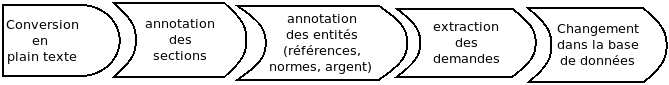
\includegraphics[width=0.8\textwidth]{pipeline-demo.png}
	\caption{Détails du module d'extraction d'information}\label{fig:demo:module-extraction}
\end{figure}

Après extraction, les décisions de la base de données sont réparties dans l'espace (ville) comme sur la figure \ref{fig:demo:doc-per-city} et dans le temps comme sur la figure \ref{fig:demo:doc-per-year}. Les demandes extraites se répartissent comme suit: 476 ACPA, 409 CONCDEL, 160 DANAIS, 0 DCPPC, 34 DORIS, et 45928 STYX.  

\begin{figure}[ht]
	\centering
	\begin{subfigure}[ht]{0.55\textwidth}
		\centering
		\centering
		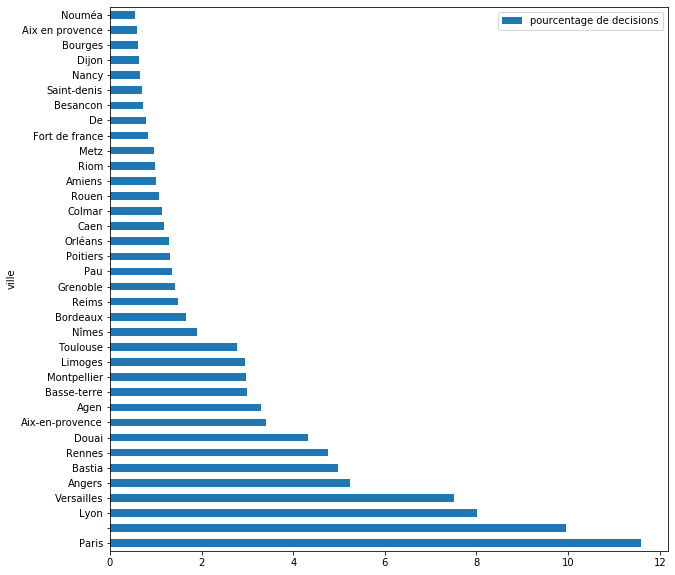
\includegraphics[width=\textwidth]{demo-pourcentage-decision-par-ville.png}
		\caption{Par ville (pourcentage>0)} \label{fig:demo:doc-per-city}
	\end{subfigure} 
	\begin{subfigure}[ht]{0.43\textwidth}
		\centering
		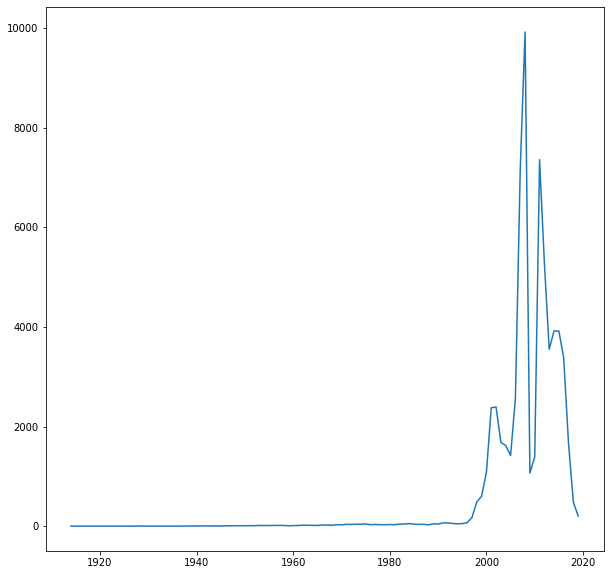
\includegraphics[width=\textwidth]{demo-repartition-decision-par-annee-1900_2019.png}
		\caption{Par an (entre 1900 et 2019)} \label{fig:demo:doc-per-year}
	\end{subfigure}
	\caption{Répartition des décisions} \label{fig:demo:docs-distribution-over-time-and-space}
\end{figure}


La structuration des données dans la base de données permet de mieux comprendre la jurisprudence à l'aide de graphiques appropriés. Une application de visualisation dédiée a notamment été développée  par \citet{PRYSIAZHNIUK2017jurisprudence-demo-web}.
Les analyses des sections suivantes sont restreintes aux 5 villes ayant les plus grands nombres de décision: Paris, Lyon, Versailles, Angers, Bastia; sur la période 2000-2019

\section{Analyse du sens du résultat}
A partir de la base des données extraites, l'évolution du pourcentage de demandes acceptées  peut être observée sur une courbe. En traçant une telle courbe pour chaque ville il est possible de comparer les villes.
Par exemple, pour les dommages intérêts sur l'article 700 du Code de Procédure Civile (STYX), la Figure \ref{fig:demo:analyse-sens-resultat-styx} compare l'évolution du sens du résultat entre les villes citées précédemment. On remarque que les demandes sont beaucoup plus rejetées qu'acceptées. La courbe du nombre total de demandes doit y être associée pour savoir si le pourcentage de succès est considérable\footnote{Pour une année où une seule demande est extraite et acceptée, le pourcentage est à 100\%, mais ce n'est pas considérable.}.

\begin{figure}[!htb]
	\centering 
	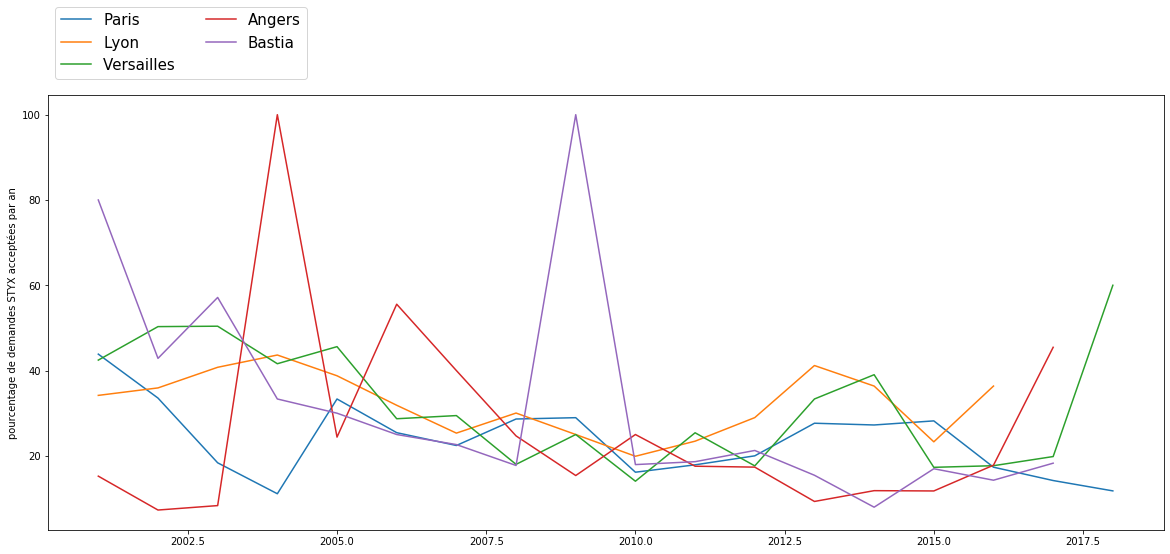
\includegraphics[width=0.9\textwidth]{evolution_sens_resultat_styx.png}
	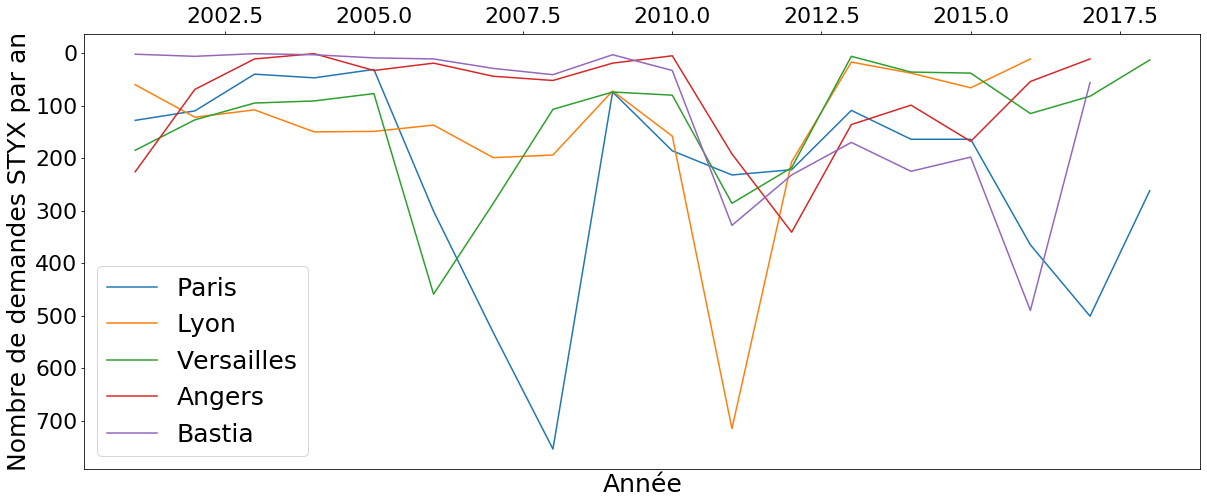
\includegraphics[width=0.9\textwidth]{evolution_nbdmd_styx.png}
	\caption{Evolution du sens du résultat des demandes STYX dans le temps à Paris, Lyon, Versailles, Angers, Bastia.}\label{fig:demo:analyse-sens-resultat-styx}
\end{figure}

La visualisation par l'application de \citet{PRYSIAZHNIUK2017jurisprudence-demo-web} permet de comparer les villes en observant sur un arbre l'épaisseur des branches associées aux catégories de demande (Figure \ref{fig:demo:web-styx}). On peut ainsi facilement observer quelles villes acceptent les demandes d'une certaine catégorie plus que d'autres par exemple.

% webdemo-sensresultat-5villes.png

\begin{figure}[!htb]
	\centering 
	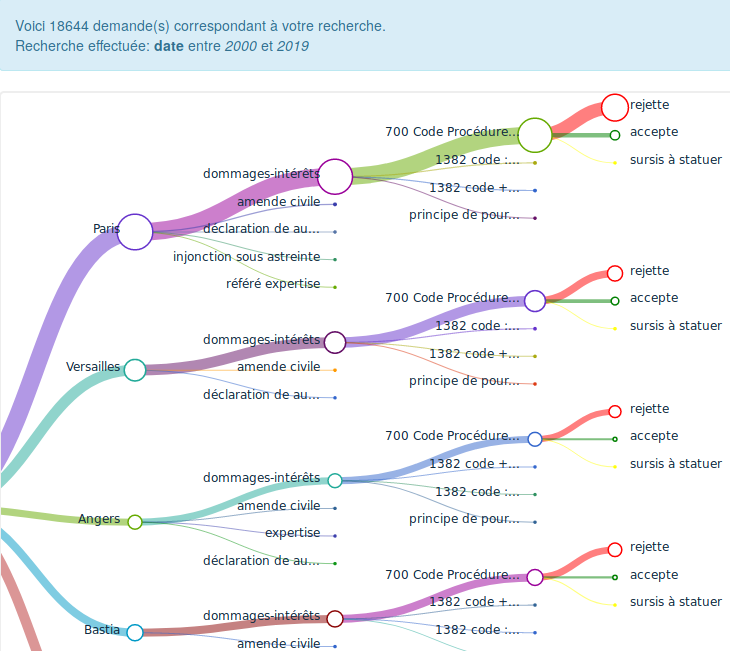
\includegraphics[width=0.6\textwidth]{webdemo-sensresultat-5villes.png}
	\caption{Comparaison des Paris, Lyon, Versailles, Angers, Bastia sur l'acceptation des demandes STYX à partir d'une visualisation arborée.}\label{fig:demo:web-styx}
\end{figure}

\section{Analyse des quanta}
\subsection{Evolution dans le temps}
De même l'évolution des quanta demandés et accordés peut être facilement visualisée par un diagramme en barre comme celui de la Figure \ref{fig:demo:evolution-quanta-styx} qui correspond aux demandes STYX entre 2000  et 2019. Même si le nombre total de demandes est à prendre en compte, un tel diagramme donne un aperçu des sommes d'argent demandés et accordés chaque année. 

\begin{figure}[!htb]
	\centering 
	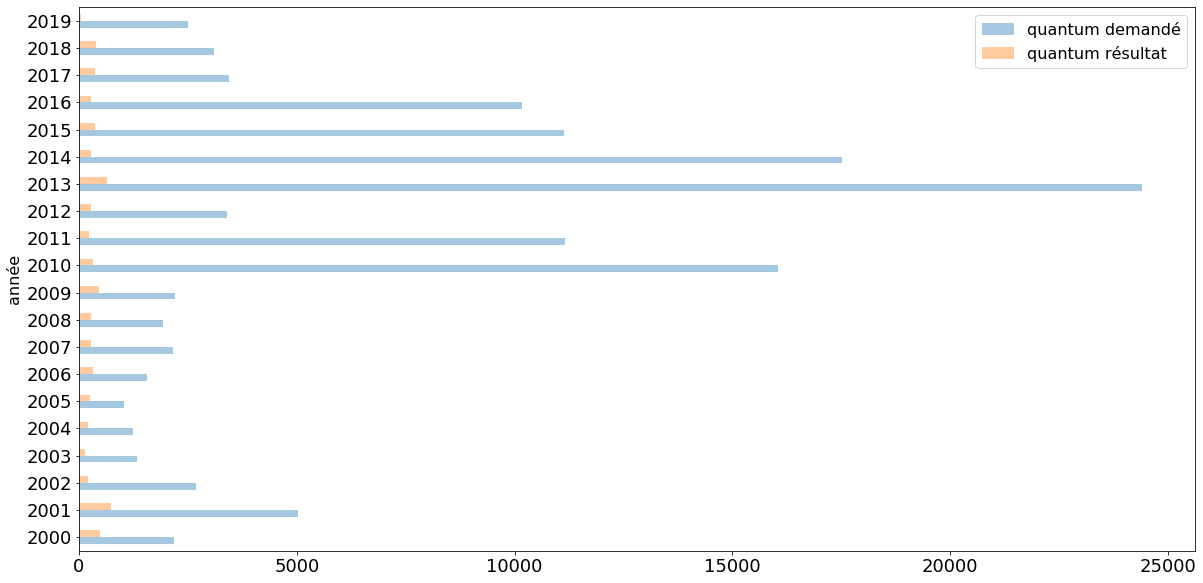
\includegraphics[width=0.8\textwidth]{evolution_quanta_styx.png}
	\caption{Evolution des quanta moyens par année des demandes STYX entre  2000  et 2019.}\label{fig:demo:evolution-quanta-styx}
\end{figure}


\subsection{Différence dans l'espace}

Pour avoir une idée du montant qu'on peut recevoir pour une catégorie de demande, l'évolution des valeurs généralement accordés peut être comparée entre deux villes en visualisant les diagrammes boîtes (\textit{boxplot}) 
des quanta accordés dans ces villes. La Figure \ref{fig:demo:evolution-qr-styx-compare-ville} permet d'effectuer une comparaison entre Bastia et Lyon. On remarque, par exemple, qu'en cas d'acceptation de la demande, il faut s'attendre à recevoir au maximum une somme autour de 5k euros à Bastia contre 10k euros à Lyon.

\begin{figure}[!htb]
	\centering 
	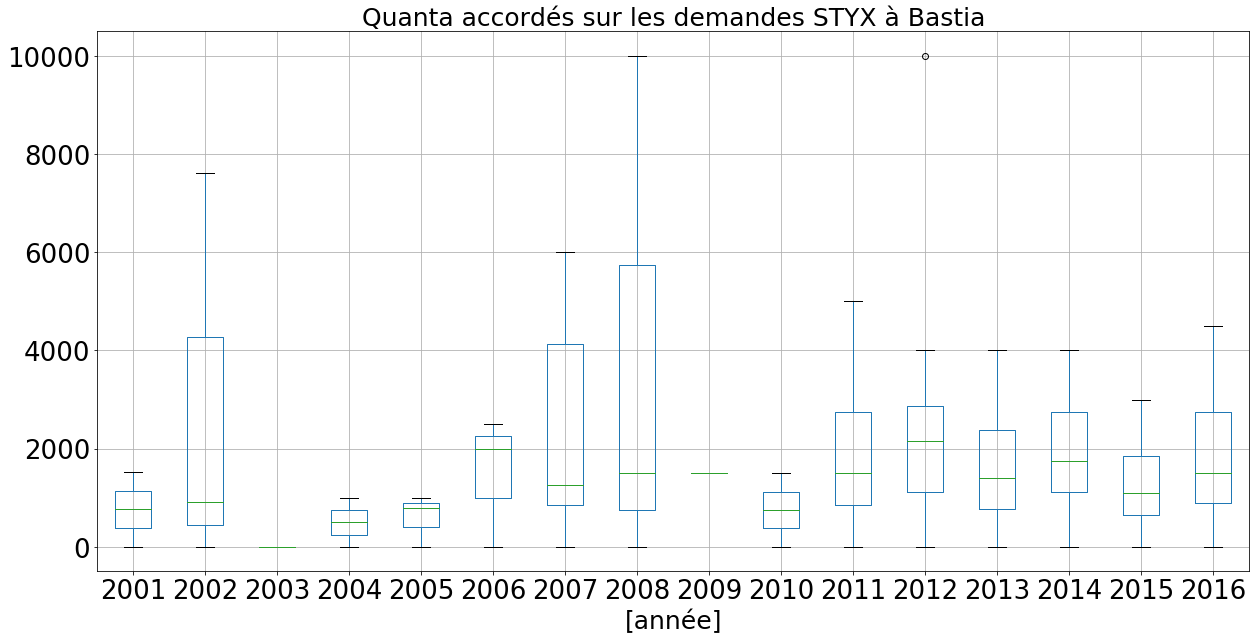
\includegraphics[width=0.6\textwidth]{qr_STYX_Bastia.png}
	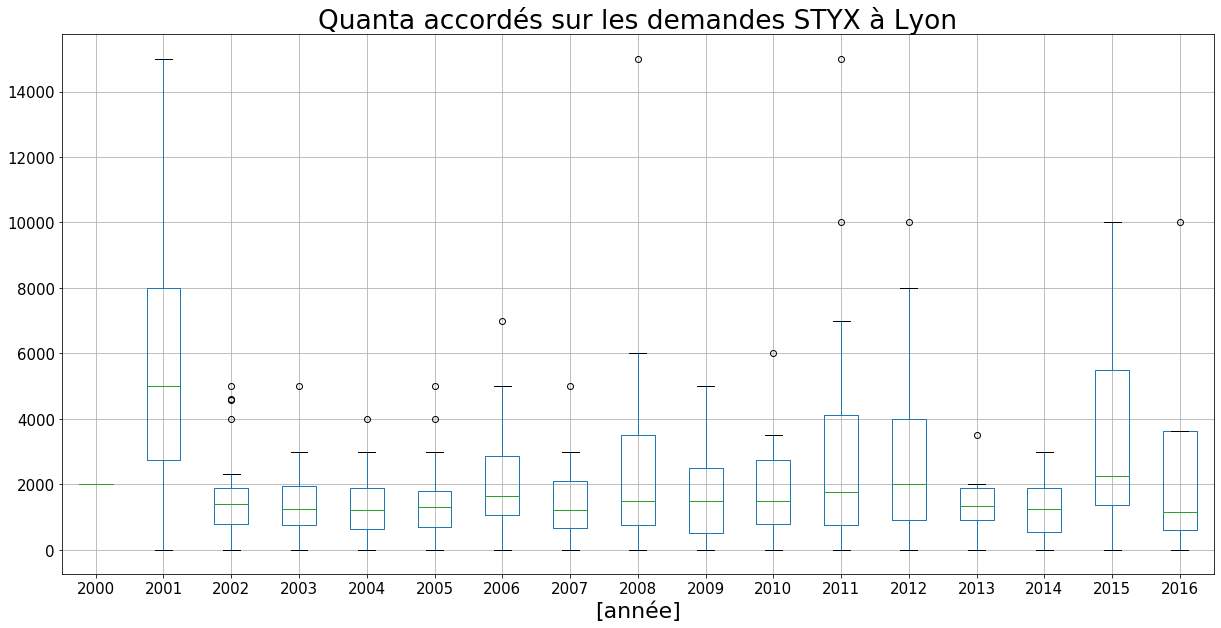
\includegraphics[width=0.6\textwidth]{qr_STYX_Lyon.png}
	\caption{Evolution des quanta accordés par année sur les demandes STYX entre 2000 et 2016 à Bastia et à Lyon.}\label{fig:demo:evolution-qr-styx-compare-ville}
\end{figure}


\subsection{Quantum demandé vs. quantum accordé}
La prédiction du quantum résultat doit définir un modèle dont la forme s'accorde avec celle du nuage de points ($x=$ quantum demandé, $y=$ quantum accordé) correspondant. D'après les nuages de points observés pour Paris, Bastia, Angers et Lyon (Figure \ref{fig:demo:qr-vs-qd-styx-compare-ville}), le quantum demandé ne semble pas suffisant seul pour déterminer le quantum accordé\footnote{Différentes valeurs de quantum résultat sont observées pour la même valeur de quantum demandé.}. Il sera ainsi nécessaire de tenir compte des circonstances factuelles et autres spécificités du cas traité qui permettront de filtrer les décisions sur lesquelles se basera l'apprentissage. On remarque néanmoins une ressemblance de forme entre les nuages de points des différentes villes. 

\begin{figure}[!htb]
	\centering 
	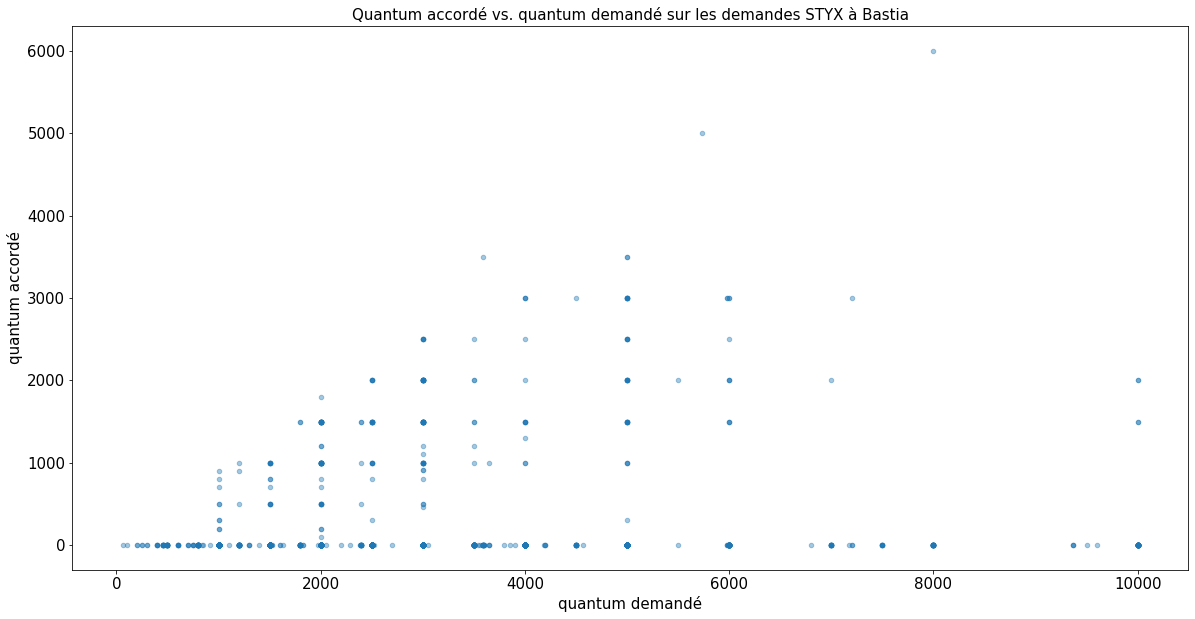
\includegraphics[width=0.47\textwidth]{qr-vs-qd_STYX_Bastia.png}
	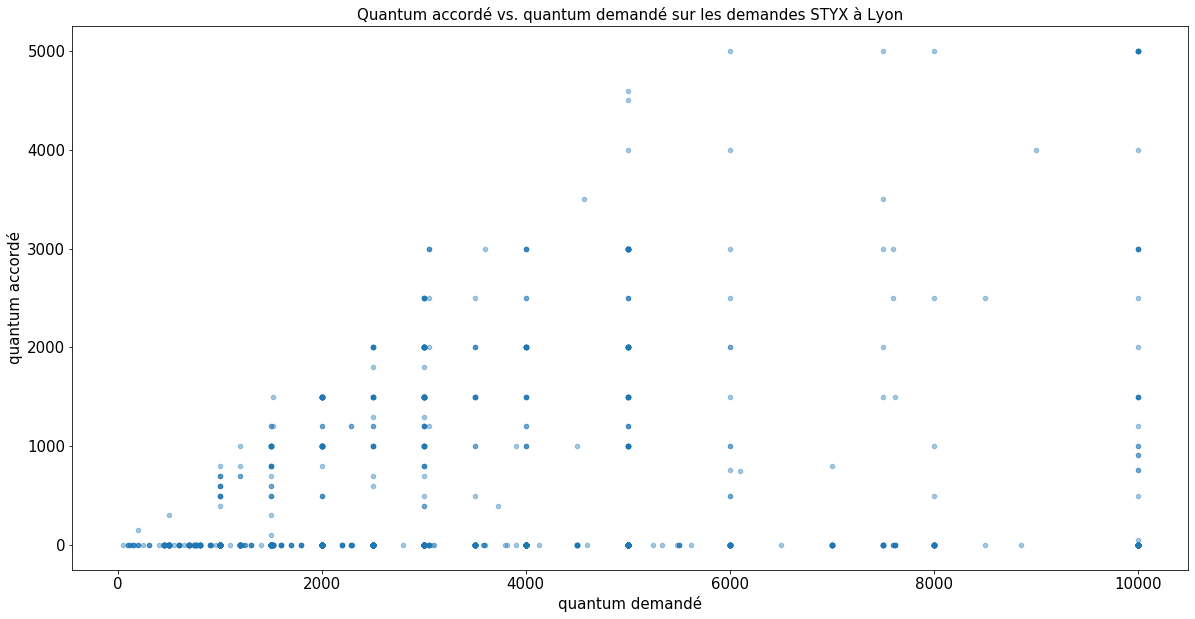
\includegraphics[width=0.47\textwidth]{qr-vs-qd_STYX_Lyon.png}
	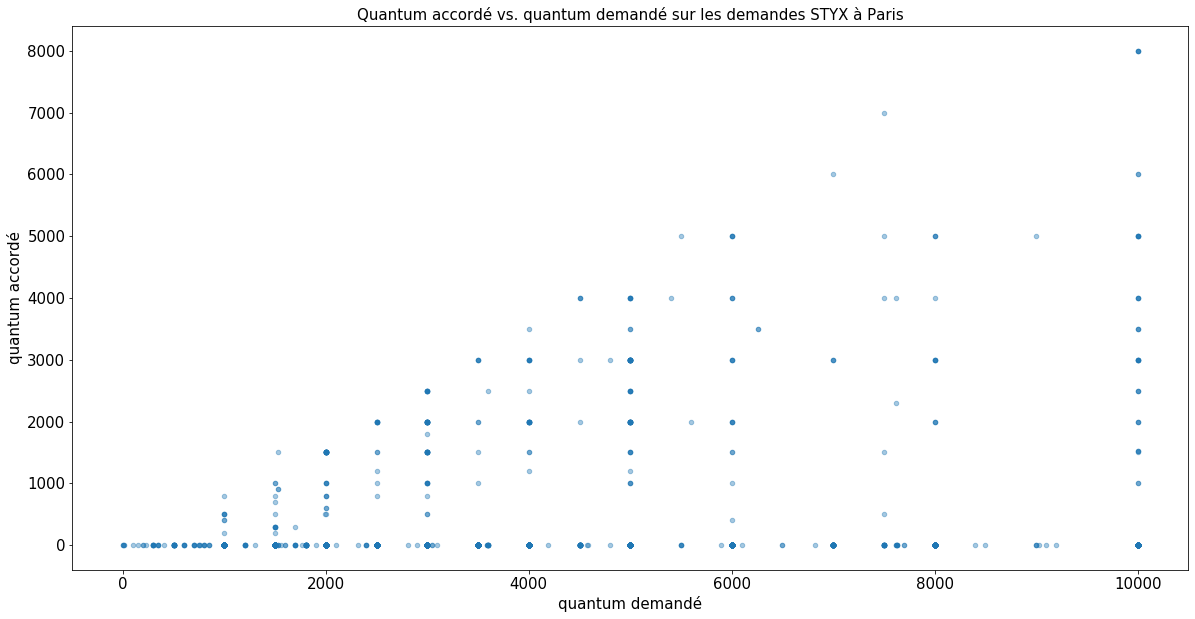
\includegraphics[width=0.47\textwidth]{qr-vs-qd_STYX_Paris.png}
	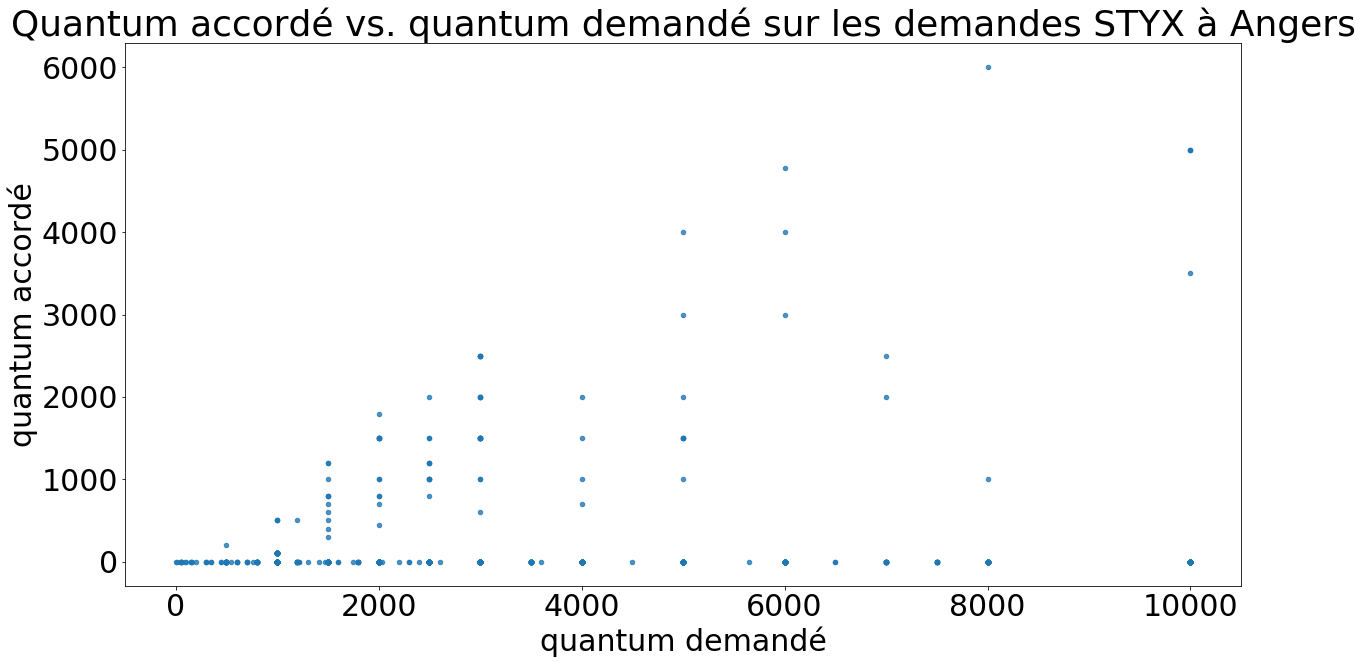
\includegraphics[width=0.47\textwidth]{qr-vs-qd_STYX_Angers.png}
	\caption{Nuages des points (quantum accordé, quantum demandé) pour les demandes STYX entre 2000 et 2019 à Paris, Bastia, Angers et Lyon (quantum demandé < 10000) .}\label{fig:demo:qr-vs-qd-styx-compare-ville}
\end{figure}

\section{Conclusion}
\label{sec:demo:conclusion}
Les démonstrations de ce chapitre donnent quelques exemples de statistiques qui informent de l'état de la jurisprudence à partir d'informations extraites à l'aide des approches proposées dans cette thèse. Les analyses du sens du résultat et des quanta sont les principales applications directes de la chaîne de traitement développée. Ce chapitre se limite aux filtres sur l'année, la ville, et la catégorie de demande, mais les analyses peuvent déjà être affinées en associant d'autres filtres comme  des mot-clés,  les normes appliqués, ou le type de juridiction. Les analyses pourront être plus riches grâce l'extraction future de nouvelles informations comme les motivations des juges et de meilleurs modèles de circonstances factuelles. % INCLUDE: demo


\backmatter

% changement du style des chapitres
\renewcommand{\chaptermark}[1]{\markboth{#1}{}}
\renewcommand*\thesection{\roman{section}}
\renewcommand*\thesubsection{\thesection.\alph{subsection}}
\setcounter{section}{0}
\makeatletter
\def\thickhrulefill{\leavevmode \leaders
	\hrule height 1ex \hfill \kern \z@}
\def\@makechapterhead#1{%
	\vspace*{10\p@}%
	{\parindent \z@
		{\reset@font
			%\usefont{OT1}{phv}{b}{n}
			\large \bf Chapitre \thechapter\par\nobreak}%
		\par\nobreak
		\vspace*{20\p@}
		\interlinepenalty\@M
		%\usefont{OT1}{ptm}{b}{n}
		{\raggedright \Large  \bfseries #1}%
		\par\nobreak
		\vskip 20\p@
		%\hrule height 2pt
		\par\nobreak
		\vskip 45\p@
}}
\def\@makeschapterhead#1{%
	\vspace*{10\p@}%
	{\parindent \z@
		{\raggedleft \reset@font
			\scshape \vphantom{\@chapapp{} \thechapter}
			\par\nobreak}%
		\par\nobreak
		\vspace*{15\p@}
		\interlinepenalty\@M
		%\usefont{OT1}{ptm}{b}{n}
		{\raggedright \Large \bfseries #1}%
		\par\nobreak
		\vskip 20\p@
		\hrule height 2pt
		\par\nobreak
		\vskip 20\p@
}}

\chapter*{Conclusion générale}
\addcontentsline{toc}{chapter}{Conclusion générale}
\label{chap:conclusion}

\textcolor{red}{Pourquoi n'avoir pas utilisé des méthodes de deep learning la thèse? disponibilité des approches de l'état de l'art, peu de données labellisées.}

\section{Évaluation des contributions}
\label{sec:conclusion:contributions}
Cette thèse  porte essentiellement sur la proposition et l'exploration d'approches adressant des problèmes d'analyses de données textuelles rencontrés lors de l'étude de corpus jurisprudentiels par des experts juristes. Trois problèmes principaux y sont abordés. Premièrement, l'annotation, dans les documents, des sections de textes et des entités nommées propres au domaine judiciaire qui peuvent aider à se repérer dans le document et à améliorer la recherche d'information. Le chapitre \ref{chap:structuration}  démontre empiriquement, sur des documents annotés pour la circonstance, l'efficacité de l'application de modèles probabilistes d'étiquetage de séquences, HMM et CRF, sur les deux tâches. Par la suite, l'extraction de données relatives aux demandes, suivant leur catégorie juridique, est discutée dans les chapitres \ref{chap:quanta} et \ref{chap:sensresultat}. Le problème impose d'effectuer les extractions pour une catégorie de demande à la fois car il est impossible d'annoter suffisamment de données pour toutes les catégories prédéfinies. Pour cela nous proposons de filtrer à l'entrée les documents de la catégorie à traiter par une classification binaire. Ensuite, il est proposé une approche ad-hoc identifiant d'une part les quanta demandés et accordés à l'aide de la position de termes clés appris sans exemple grâce à des métriques de pondération des termes, et d'autre part le sens du résultat à l'aide d'un ensemble prédéfini de mots-clés particulier à la rédaction des résultats. Cette méthode, bien que dépendante d'heuristiques, parvient à reconnaître un grand nombre de demandes avec plus ou moins de difficultés selon les catégories traitées. Ensuite, la classification de documents est expérimentée comme approche plus généraliste. Sur l'ensemble des algorithmes explorés, les extensions de l'analyse PLS, appliquées ici pour la première fois sur du texte, démontrent une efficacité proche de celle du meilleur algorithme testé, l'arbre de décision.  L'utilité de la restriction des documents à des passages relatifs à la catégorie est aussi démontrée empiriquement. Enfin, le chapitre \ref{chap:similarite} aborde la problématique de similarité entre deux textes dans un contexte de catégorisation non supervisée des documents. Le but est ici de révéler les circonstances factuelles faisant appel à une catégorie de demande particulière. Une approche d'apprentissage de distance est proposée: elle repose sur le coût d'une transformation d'un des deux textes en l'autre.
Cette distance est comparée à d'autres métriques avec l'algorithme des K-moyennes dans des expérimentations qui explorent différents aspects des problèmes de regroupement comme la détermination du nombre de clusters ou la représentation de documents. En somme, les problématiques abordées sont certes variées mais indispensables aux différents maillons de la chaîne complète de traitement automatique de corpus de décisions dont le chapitre \ref{chap:demo} montre l'utilité pour visualiser l'état de la jurisprudence, une des nombreuses applications possibles des données extraites. 


\section{Critique du travail}
\label{sec:conclusion:critique}
Au delà des nombreuses problématiques abordées et expérimentations discutées, cette thèse reste limitée par son niveau de contribution théorique d'une part. La proposition globale est une chaîne de traitement employant à chaque niveau des approches soit existantes soit plus techniques. Aussi, un très grand nombre de méthodes de la littérature sont absentes, surtout les plus récentes; ceci est dû fait à l'ampleur du travail et à la multitudes d'approches existantes.  D'autre part, les études menées ont rencontrées comme obstacles la disponibilité d'exemples de référence annotées manuellement. La lenteur et la pénibilité de l'identification des informations à la main se traduit par la faible quantité des données employées pour les expérimentations. De plus, ne disposant que d'un expert, le degré d'accord entre annotateurs n'a été analysé que pour la première problématique de reconnaissance d'entités et de sections. Par conséquent, certaines subtilités propres à l'expert ou des données manquées lors de l'annotation manuelle, peuvent biaiser les résultats observés. Néanmoins, les nombreux résultats obtenus servent de base pour la continuité des études. 


\section{Travaux futurs de recherche}
\label{sec:conclusion:extensions}
Les propositions données dans la conclusion des chapitres \ref{chap:structuration} à \ref{chap:demo} pour continuer les travaux peuvent être résumées en 4 catégories principale. En premier, l'exploration de méthodes récentes que celles étudiées permettra d'étendre les résultats expérimentaux. Ensuite, la formalisation des problèmes abordées permettra de définir des approches plus théoriques. Par exemple, la formalisation des demandes comme des relations, entre quantum demandé et quantum accordé, permettra d'explorer le cadre probabiliste et neuronale de la littérature en matière d'extraction des relations. Puis, l'exploration d'autres formulation des problèmes permettra probablement de découvrir des méthodes plus efficaces. Par exemple, on peut percevoir la détermination des circonstances factuelles comme une tâche de modélisation de thématiques (\textit{topic modeling}). Enfin, l'exploration plus approfondie d'autres aspects des problèmes. Par exemple, la reconnaissance d'entités nommées comprend l'identification que nous avons étudiée, et la résolution qui unifie les mentions variantes d'une entité sous un identifiant prédéfinir ou à définir automatiquement.

Il faut aussi remarquer qu'il reste encore des types d'information dont le problème d'extraction n'est pas abordé par cette thèse. Par exemple, les raisons, qui  font penchés les juges en faveur d'une décision sur une demande, sont indispensables pour être capable d'anticiper la prise de décision des juges. L'extraction des raisons concernera l'identification et l'analyse des arguments des parties et les motivations des juges.

 Par ailleurs, il faudra aussi mieux évaluer la qualité des annotations manuelles expertes ce qui révélera le niveau d'accord non seulement sur les données annotées mais aussi sur leur perception des informations ciblées comme les circonstance factuelles qui semblent subjectives. 

\section{Perspectives du domaine}
\label{sec:conclusion:perspectives}

D'une part, le conflit entre la qualité des données annotées manuellement et la rapidité de l'automatisation encore imprécise est important. \cite{Galgani2015lexa} supportent, par exemple, qu'il est possible en un temps raisonnable d'annoter manuellement un nombre considérable de texte. Il se pose alors la question de savoir à quel point l'exhaustivité est-elle nécessaire pour contraindre les experts à supporter la marge d'erreurs infligée par les outils d'extraction automatique.

D'autre part, cette thèse est l'un des premiers travaux de recherche de cet largeur sur les décisions françaises. Ainsi, elle ouvre la voie à bien des problématiques comme l'analyse des réseaux de normes, l'anonymisation des décisions, ou l'analyse des arguments, déjà largement étudiés dans d'autres pays, notamment aux États-Unis. En cela, cette thèse encourage la recherche en analyse de donnée textuelle à s'intéresser à l'analyse automatique de la jurisprudence française dont les défis, la disponibilité d'un grand volume de données et la lucrativité du domaine judiciaire ne rendent ce champ d'application que plus attractif. Les cas d'utilisation des données extraites sont très nombreuses dans la recherche en droit, l'aide à la décision des juristes, dans l'enseignement du droit, et surtout dans l'accessibilité des profanes au droit par une estimation automatique de leurs risques judiciaires.
 % INCLUDE: conclusion

%Bibliographie
\def\bibname{Bibliographie}
\addcontentsline{toc}{chapter}{\bibname}
\bibliography{bib/references-pub}

%\newpage
%Glossaire
%\printnomenclature[2cm]
%\addcontentsline{toc}{chapter}{\nomname}
%Annexes
%annexes
%\appendix
%\begin{appendices}
%\chapter{Recherche d'Articles Juridiques (COLIEE2017)}
\label{chap:coliee}
\section{Description de la Tâche de Recherche d'Information}

\section{Application de Métriques de Recherche d'Information}

\section{Application de la Classification de Texte}

%\chapter{SDZE} % INCLUDE: coliee
%\end{appendices}
\end{document}